
\documentclass[czech,master]{diploma}
% Dalsi doplnujici baliky maker
\usepackage[autostyle=true,czech=quotes]{csquotes} % korektni sazba uvozovek, podpora pro balik biblatex
\usepackage[backend=biber, style=iso-numeric, alldates=iso]{biblatex} % bibliografie
\usepackage{dcolumn} % sloupce tabulky s ciselnymi hodnotami
\usepackage{subfig} % makra pro "podobrazky" a "podtabulky"
\usepackage[cpp]{diplomalst}



\usepackage{multirow}
\usepackage{pgfplots}
\pgfplotsset{compat=newest}
\usepackage{amsmath}

\usepackage{pgffor}
\usepackage{catchfile}
\usepackage{svg}

% Novy druh tabulkoveho sloupce, ve kterem jsou cisla zarovnana podle desetinne carky
\newcolumntype{d}[1]{D{,}{,}{#1}}



% Zadame pozadovane vstupy pro generovani titulnich stran.
\ThesisAuthor{Bc. Filip Łuński}

\ThesisSupervisor{Ing. Tomáš Wiszczor, Ph.D.}

\CzechThesisTitle{Využití kamerového systému pro zajištění bezpečnosti osob na pracovišti}

\EnglishThesisTitle{Use of Surveillance Cameras to Ensure the Safety of People in the Workplace}

\SubmissionYear{2025}

\ThesisAssignmentFileName{ThesisSpecification_LUN0024_vsboee2404016E.pdf}


% \Acknowledgement{Rád bych na tomto místě poděkoval všem, kteří mi s prací pomohli, protože bez nich by tato práce nevznikla.}


\CzechAbstract{ Rozvoj technologie v posledních letech, zejména v oblasti umělé inteligence a neuronových sítí, umožňuje komplexnější analýzy chování osob. Dalo by se tak bezpečnostní kamery využít pro zajištění bezpečnosti osob. V této práci je tak navrženo řešení pro detekci pádu osob v obrazovém toku v reálném čase. Řešení je postaveno na kombinaci dvou neuronových sítí. První detekuje všechny osoby v obraze a jejich klíčové body, druhá tyto body klasifikuje do tříd "normální" a "upadl". V práci je popsán výběr detektoru pózy, návrh architektury klasifikační sítě a implementace výsledného detektoru pádu. Ve výsledném řešení je použit model YOLO11-pose a rekurenetní neuronová síť postavená na architektuře GRU. }

\CzechKeywords{python, strojové učení, neuronové sítě, konvoluční neuronové sítě, rekurentní neuronové sítě, GRU, LSTM, PyTorch, detekce pozy, detekce chování, detekce pádu, YOLO  }

\EnglishAbstract{The development of technology in recent years, particularly in the field of artificial intelligence and neural networks, enables more complex analyses of human behavior. Security cameras could thus be used to ensure personal safety. This work proposes a solution for real-time detection of human falls in video streams. The solution is based on a combination of two neural networks. The first detects all people in the image and their key points, the second classifies these points into the categories "normal" and "fallen". The work describes the selection of a pose detector, the design of the classification network architecture, and the implementation of the resulting fall detector. The final solution uses the YOLOv11-pose model and a recurrent neural network based on the GRU architecture.}

\EnglishKeywords{python, machine learning, neural networks, convolutional neural networks, reccurent neural networks, GRU, LSTM, PyTorch, pose estimation, behaviour detection, fall detection, YOLO }

% Seznam zkratek a symbolů 

\AddAcronym{NN}{Neural network - neuronová síť}
\AddAcronym{ANN}{Artificial neural network - umělá neuronová síť}
\AddAcronym{CNN}{Convolutional neural network - konvoluční neuronová síť}
\AddAcronym{RNN}{Recurrent neural network - rekurentní neuronová síť}
\AddAcronym{LSTM}{Long short-term memory - dlouhá krátkodobá paměť}
\AddAcronym{AI}{Artificial intelligence - umělá inteligence}
\AddAcronym{ML}{Machine learning - strojové učení}
\AddAcronym{DL}{Deep learning - hluboké učení}



\AddAcronym{ReLU}{Rectified Linear Unit}
\AddAcronym{LeakyReLU}{Leaky Rectified Linear Unit}
\AddAcronym{ELU}{Exponential Linear Unit}
\AddAcronym{SELU}{Scaled Exponential Linear Unit}
\AddAcronym{GELU}{Gaussian Error Linear Unit}
\AddAcronym{GD}{Gradient Descent}
\AddAcronym{SGD}{Stochastic Gradient Descent}
\AddAcronym{MBSGD}{ Mini-Batch Stochastic Gradient Descent}
\AddAcronym{NAG}{Nesterov Accelerated Gradient}
\AddAcronym{AdaGrad}{Adaptive Gradient}
\AddAcronym{RMSprop}{Root Mean Square Propagation}
\AddAcronym{Adam}{Adaptive Moment Estimation}
\AddAcronym{AdamW}{Adam with Weight Decay}
\AddAcronym{Nadam}{Nesterov-accelerated Adaptive Moment Estimation}
\AddAcronym{BP}{Backpropagation}
\AddAcronym{BN}{Batch Normalization}
\AddAcronym{DO}{Dropout}
\AddAcronym{LR}{Learning Rate}
\AddAcronym{MSE}{Mean Squared Error}
\AddAcronym{BCE}{Binary Cross-Entropy}
\AddAcronym{CCE}{Categorical Cross-Entropy}
\AddAcronym{TL}{Transfer Learning}
\AddAcronym{FT}{Fine-Tuning}
\AddAcronym{WD}{Weight Decay}
\AddAcronym{ES}{Early Stopping}
\AddAcronym{LRS}{Learning Rate Scheduling}
\AddAcronym{CG}{Conjugate Gradient}
\AddAcronym{QN}{Quasi-Newton Methods}

\endinput

% Vlozeni bibliografie
\addbibresource{biblatex.bib}


% Zacatek dokumentu
\begin{document}

% Nechame vysazet titulni strany.
\MakeTitlePages

% Jsou v praci obrazky nebo tabulky? Pokud ano vysazime jejich seznam a odstrankujeme.
% Pokud ne smazeme nasledujici dve makra.
\listoffigures
\clearpage

\listoftables
\clearpage

% A nasleduje text zaverecne prace.
\chapter{Úvod}
\label{sec:Introduction}

Kamerové systémy jsou využívány již mnoho let a jejich využití je stále širší.
Dnes se odhaduje, že celkový počet bezpečnostních kamer ve světě přesahuje
miliardu. Využívány jsou v průmyslu, dopravě, obchodě, veřejných prostorech,
zdravotnictví či domácnostech.

Zpočátku bylo možné video sledovat pouze živě, později, s příchodem videokazet,
bylo možné záznam sledovat až po události. Digitální éra a síťové kamery
umožnily přístup ke kamerovým záznamům z libovolného místa na světě. V poslední
době se také začalo nahrazovat živé sledování automatickým zpracováním obrazu a
detekcí událostí s využitím technik umělé inteligence.

Kamerové systémy se používají zejména ve dvou oblastech: zabezpečení (.
security), myšleno jako ochrana před úmyslnými hrozbami a protiprávními činy,
jako jsou krádeže, poškozování majetku, či neoprávněný vstup; a bezpečnost
(ang. safety), což zahrnuje ochranu před nehodami a náhodnými hrozbami, jako
jsou pády, požár, úniky nebezpečných látek, či porušování bezpečnostních
předpisů.

Jak již bylo zmíněno, lze kamery využívat jednak pro živé sledování, jednak pro
záznam a jeho analýzu po události. Kamerové záznamy jsou zejména důležité pro
zpětnou analýzu incidentů, důkazní materiál pro soudní spory, zjišťování příčin
nehod, či pro zlepšení bezpečnostních opatření. Živé sledování videa se pak
snaží incidentům přímo předcházet. Bylo však prokázáno, že schopnost lidského
pozorovatele detekovat nebezpečí se velmi snižuje s délkou sledování a s počtem
monitorovaných kamer. Právě proto se s příchodem technik umělé inteligence
začalo využívat automatické zpracování obrazu a detekce hrozeb, nebezpečí, nebo
již probíhajících incidentů v jejích počátcích. Tyto techniky pak úplně
nahrazují lidského pozorovatele, nebo mu pomáhají včas zpozorovat nebezpečí a
zareagovat.

Automatická analýza obrazu je používaná již několik desítek let, většinou ale
spíše pro oblast zabezpečení, než pro bezpečnost. To z toho důvodu, že úlohy,
jako identifikace neoprávněného vstupu, detekce zbraní, rozpoznávání SPZ nebo
podezřelých osob jsou pro algoritmy mnohem jednodušší, než například detekce
pádu, nouzové situace či zdravotního problému. Hlavním problémem těchto
komplexnějších analýz je vysoká falešná pozitivita, kdy je například těžké
rozeznat člověka trénujícího běh od člověka utíkajícího před nebezpečím.
Nicméně rozvoj v oblasti hlubokého učení a konvolučních neuronových sítí, jako
i vývoj a dostupnost hardwaru podporujícího tyto techniky, umožňuje dneska
využít je i pro složitější úlohy.

Ve firmě Linde jsou kamerové systémy používány v mnoha průmyslových provozech,
nicméně chybí ucelený systém pro automatickou analýzu obrazu a detekci různých
druhů nebezpečí. Naším úkolem tedy v budoucnu bude navrhnout a implementovat
modulární systém s možností sledování konkrétních nebezpečí na konkrétních
místech. Ty budou zahrnovat například detekci pádu, požáru, zdravotních
problémů, nebo porušování bezpečnostních opatření. Systém pak bude v případě
rozpoznání nějaké hrozby informovat příslušného pracovníka.

V této práci se zaměříme pouze na jednu z těchto úloh, a to na detekci pádu.
Pád může mít různé příčiny, ať už je to zdravotní problém jako ztráta vědomí,
nebo zakopnutí. Někdy se zdá, že samotné zakopnutí je banální problém, nicméně
pokud se na pracovišti nenachází nikdo, kdo by mohl pomoct, a poškozený není
schopen sám přivolat pomoc, může vést takový incident k vážným následkům.

V první části práce se budeme zabývat teoretickými základy, jako je obecná
architektura neuronových sítí či princip konvolučních neuronových sítí. V
dalších kapitolách se zaměříme na detekci osob a odhad jejich klíčových bodů.
Projdeme si různé přístupy a otestujeme různé algoritmy s ohledem na výkon,
možnou hardwarovou akcelerací a preciznost. V další části se budeme zabývat
samotnou detekcí pádu, tedy algoritmem, který na základě odhadnutých klíčových
bodů určí, zda došlo k pádu, či nikoliv. V závěru práce se zaměříme na
otestování výsledného řešení a zhodnocení jeho výkonu.

\endinput
% \part{Teorie}
\chapter{Krátké seznámení s neuronovými sítěmi}
\label{chap:NN}

Umělá neuronová síť (ang. artificial neural network – ANN) nebo jen neuronová
síť (ang. neural network – NN) je výpočetní model inspirovaný biologickými
nervovými systémy v lidském mozku. Na rozdíl od konvenčních výpočetních modelů,
které zpracovávají informace algoritmicky, a tedy postupují dle předem určeného
postupu, se informace v tomto modelu šíří paralelně v síti vah mezi
jednotlivými neurony. Jelikož je výstup ze sítě dané architektury závislý
hlavně na numerických parametrech, zejména váhách jednotlivých spojů mezi
neurony, lze funkčnost sítě měnit bez změny programu pouhou změnou těchto
parametrů, a to i automaticky v procesu trénování modelu.

Jelikož budou neuronové sítě základem prakticky v každé fázi vývoje
navrhovaného řešení, budou v následující kapitole popsány její základní
principy. Dále bude pozornost věnována dvěma pokročilejším architekturam
neuronových sítí: konvolučním neuronovým sítím, na kterých jsou postaveny
algoritmy pro detekci klíčových osob v obraze, a rekurentním neuronovým sítím,
jež budou použity pro analýzu klíčových bodů v sekvencích snímků.

\section{Historie}
\label{sec:NN_History}

\subsubsection*{Prvopočátky}
První matematický model neuronové sítě byl popsán v roce 1943 dvěma
neurofyziology – Warrenem McCullochem a Walterem Pittsem \cite{McCulloch1943}.
Model byl založen na síti jednoduchých logických prvků, které provedou vážený
součet svých vstupů a na výstup odešlou signál založený na prahové funkci.

V roce 1958 pak Frank Rosenblatt představil elektronický model neuronové sítě.
Základní jednotku, postavenou na McCulloch-Pittsově modelu, nazval perceptron.
\cite{Rosenblatt1958} Jeho architektura byla podobná modelu znázorněnému na
obrázku \ref{fig:neuron}, kde aktivační funkce je prahová funkce. Rosenblattův
stroj – Mark I Perceptron – byl postavený pro rozpoznávání jednoduchých vzorů v
obrazech.
% Hlavním omezením tohoto modelu bylo, že byl schopen rozlišovat pouze lineárně separovatelné třídy. 
Samotný model perceptronu je dodnes používán jako základ pro mnoho neuronových
sítí.

% Další systém – ADALINE (Adaptive Linear Neuron) – byl představen Bernardem
% Widrowem a Tedym Hoffem v roce 1960. Tento model umělého neuronu byl velmi
% podobný perceptronu, na rozdíl od něj ale neobsahoval prahovou ale lineární
% funkci, výstup tedy nebyl binární ale spojitý. Pro učení pak byla využita
% metoda nejmenších čtverců, která minimalizovala chybu mezi skutečným a
% očekávaným výstupem \cite{nn_history}.

I když ve svých počátcích přitahoval koncept umělé inteligence mnoho vědců jako
i sponzorů, v následujících letech zájem ochabl, jelikož nebylo dosaženo
předpokládaných výsledků, hlavně s ohledem na tehdejší stav vývoje hardwaru a
obecně výpočetní techniky. Proto se tomuto období někdy říká AI Winter.
Neznamená to ale, že ti, kteří se oboru nadále věnovali, nedosáhli významných
výsledků \cite{nn_history}.

\subsubsection*{Backpropagation}
Významným milníkem v historii neuronových sítí byl objev algoritmu
backpropagation, zvaného také algoritmus zpětného šíření chyby. Tento
algoritmus byl vyvinut v roce 1974 Paulem Werbosem, popularitu ale dosáhl až po
nezávislém objevení v roce 1986 Davidem Rumelhartem et al.
\cite{backpropagation}.

Tento algoritmus umožnil trénovat sítě s více vrstvami, což položilo základ
hlubokému učení. Algoritmus využívá metodu gradientního sestupu v kombinaci s
řetězovým pravidlem derivací k nalezení optimálních vah sítě vedoucích k
minimalizaci chyby.

Vynález backpropagation byl jedním z hlavních důvodů, proč se v 80. letech
obnovil zájem o neuronové sítě a umělou inteligenci obecně. V roce 1989 také
umožnil Yann LeCunovi et al. zefektivnit použití konvolučních neuronových sítí
pro rozpoznávání rukou psaných číslic \cite{lecun1989} a položit tak základ
širokému využití konvolučních sítí v oblasti počítačového vidění.

\section{Obecná architektura neuronové sítě}

V následující části budou popsány obecné principy fungování neuronových sítí,
jejich struktura a základní optimalizační techniky.

\subsection{Struktura neuronové sítě}

Umělé neuronové sítě jsou silně inspirované biologickými neuronovými sítěmi. A
i když napodobení celé funkčnosti lidského nervového systému by bylo velmi
složité – ne-li nereálné, zejména s ohledem na počet neuronů a způsob jejich
propojení – je možné simulovat alespoň některé funkce lidské mysli.

% Pro provádění výpočtů využívají neuronové sítě distribuovaný, paralelní
% přístup. Informace jsou tedy zpracovány, předávány a ukládány celou sítí,
% nikoliv pomocí určitých paměťových buněk. Většina znalostí je uložena v silách
% vazeb mezi jednotlivými neurony. Vazby, které vedou k úspěšnému řešení
% problému, jsou posilovány, naopak ty, které vedou k neúspěchu, jsou oslabovány.

Podstatnou vlastností neuronových sítí je jejich schopnost učení. Tato
vlastnost způsobuje, že již není nutná algoritmizace řešené úlohy, ale stačí
neuronové síti opakovaně předložit příklady popisující daný problém, podle
kterých jsou postupně upravovány síly vazeb v síti. Tato fáze učení pak určuje,
jakým způsobem bude síť transformovat vstupní data na výstupní
\cite{Vondrak1994}.

\subsection{Neuron}
Biologický neuron se skládá ze tří hlavních částí. Dendrity přijímají vstupní
signály. V těle jsou vstupní signály sečteny do jednoho potenciálu, který vede
k vybuzení neuronu – zaslání signálu na výstup, pokud potenciál překročí
určitou mez. Axonové vlákno pak vede k synapsím, tedy spojům s dalšími neurony.
Lidská mysl pak funguje na principu posilování nebo oslabování těchto spojů.

Umělý neuron se snaží tuto funkčnost napodobit, viz obrázek \ref{fig:neuron}.
Jeho vstupy $x_i$ jsou násobeny váhami $w_i$, které reprezentují sílu daného
spoje. Neuron pak tyto vážené vstupy sečte, a na tento součet aplikuje
aktivační funkci (AF), která definuje hodnotu výstupu $y$. Existuje mnoho
různých AF, v navrhovaném řešení budou vyzkoušeny například hyperbolický tangens (tanh),
ReLU či Mish \cite{afreview}.

Kromě vah jednotlivých vstupů neuron obvykle obsahuje ještě tzv. bias (někdy
také práh nebo posun), jehož funkcí je posunout vážený součet vstupů tak, aby
bylo možné modelovat i funkce, které nejsou nulové v počátku souřadnic. Je buď
reprezentován jako samostatný parametr, nebo jako váha konstantního vstupu s
hodnotou 1, jako na obrázku \ref{fig:neuron}.

% Funkci umělého neuronu lze tedy formálně vyjádřit takto:

% \begin{equation*}
%     y=f\left(\sum_{i=0}^{n}w_{i}x_{i}\right)
% \end{equation*}

% kde $w_0$ je bias a $x_0=1$, anebo s osamostatněným biasem takto:

% \begin{equation*}
%     y = f\left(\sum_{i=1}^{n} w_i x_i + b\right)
% \end{equation*}

% kde $b$ je bias.

Obecně tvoří všechny vstupní váhy a bias množinu parametrů, které ovlivňují
funkčnost celé neuronové sítě. Proces trénování sítě pak spočívá v nalezení
optimálních hodnot těchto parametrů, které vedou k co nejmenší chybě při řešení
úlohy.

\begin{figure}[]
    \centering
    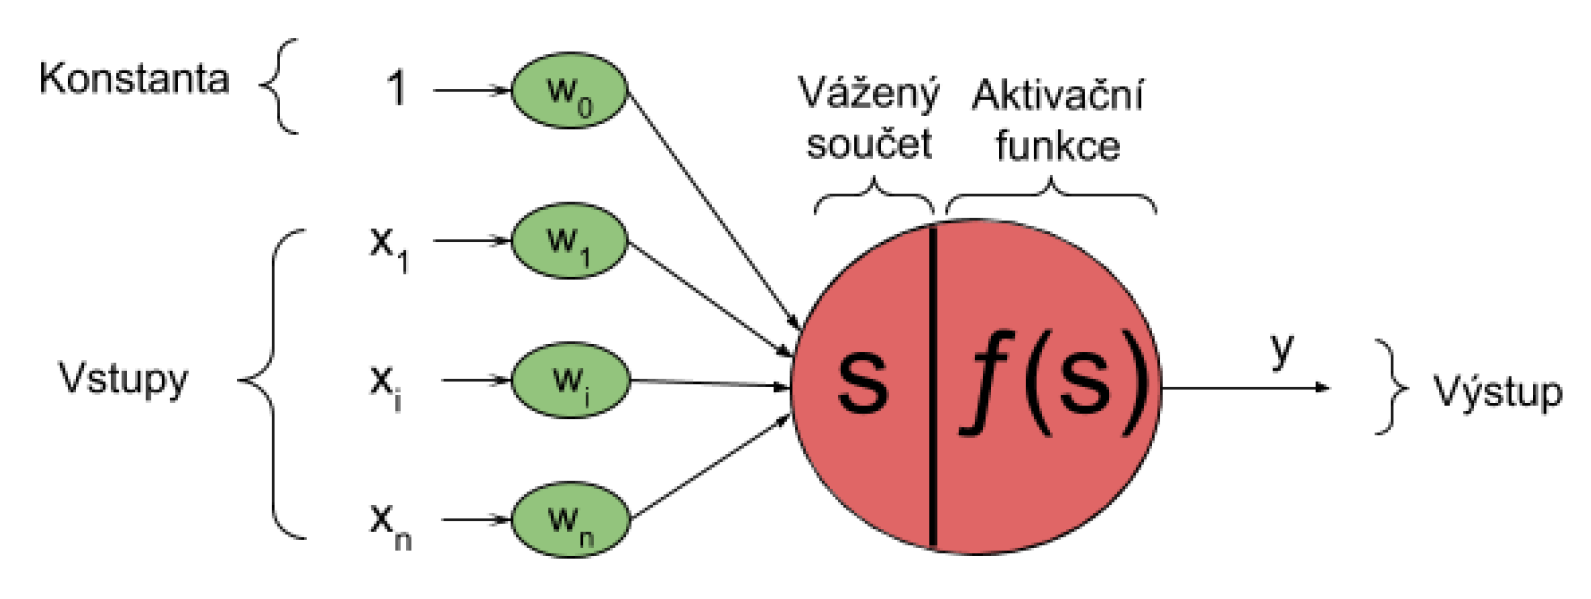
\includegraphics[width=0.7\textwidth]{Figures/neuron.png}
    \caption{Model umělého neuronu \cite{lagan}}
    \label{fig:neuron}
\end{figure}

% \subsection{Základní aktivační funkce}

% AF hraje stěžejní roli v umělých neuronových sítích zavedením nelinearity do
% celého systému a umožňuje tak učení se složitějších vzorců.

% V průběhu let bylo vyvinuto mnoho typů AF, a i když jejich úloha se zdá být
% podobná, můžou se od sebe výrazně lišit. Jejich rozdíly spočívají zejména v
% oboru hodnot, spojitosti, monotónnosti, a v tom, zda je závislá na přídavných
% trénovaných parametrech. Ve výsledku se také liší i jejich využití. Nyní
% projdeme několik základních AF, od kterých se většina ostatních nějakým
% způsobem odvíjí.

% Sigmoida (lineární křivka) funkce transformuje vstup do rozmezí 0 ÷ 1, je tak
% vhodná pro odhad pravděpodobnosti \cite{sigmoidImplementation}. Proto se také
% někdy používá ve výstupních vrstvách síti, zejména pro binární klasifikaci.
% Její funkčnost lze formálně zapsat takto:

% \begin{equation*}
%     f(x)= \frac{1}{1+e^{-x}}
% \end{equation*}

% Její nevýhodou je hlavně problém mizejícího gradientu (ang. vanishing
% gradient), kdy zejména ve vícevrstvých sítích se velikost změn váh v
% počátečních a koncových vrstvách významně liší. To pak způsobuje nestabilitu v
% procesu trénování a může jej zpomalit nebo zcela zastavit. Navíc to, že není
% nulová v počátku souřadnic, může způsobit špatnou konvergenci.

% Hyperbolický tangens (tanh) je velmi podobný sigmoidě, ale transformuje vstup
% do rozmezí -1 ÷ 1 \cite{afreview}. Řeší tedy poslední zmíněný problém. Nicméně
% se pořád potýká s problémem mizejícího gradientu. Formálně lze tuto AF popsat
% takto:

% \begin{equation*}
%     f(x)= \frac{e^x-e^{-x}}{e^x+e^{-x}}
% \end{equation*}

% Obě dříve zmíněné funkce představují větší výpočetní nároky. ReLU (Rectified
% Linear Unit, také někdy rampa) je naopak jednoduchá, zároveň ale velice
% efektivní. Pro kladné hodnoty se chová jako identita, pro záporné je nulová
% \cite{reluAnalysis}.

% \begin{equation*}
%     f(x)=\max(0,x)=\begin{cases}x&x>0,\\0&x\leq0,\end{cases}
% \end{equation*}

% Jelikož je výpočetně velmi nenáročná, je tato AF velmi oblíbená v hlubokých
% sítích. Její nevýhodou ale je, že nezohledňuje záporné hodnoty, což v jejich
% případě vede k problému mizejícího gradientu a může způsobit tzv. "mrtvé
% neurony". Tento problém řeší různé varianty ReLU, jako například PReLU
% (Parametric ReLU) nebo LReLU (Leaky ReLU). Tyto varianty přidávají parametr $p$
% vynásobený $x$ pro záporné hodnoty:

% \begin{equation*}
%     f(x)=\max(0,x)=\begin{cases}x&x>0,\\p \cdot x&x\leq0\end{cases}
% \end{equation*}

% LReLU má tento parametr fixně nastavený na $p=0.01$, zatímco v případě PReLU je
% tento parametr trénovaný spolu s jinými parametry sítě.

% Další novější alternativou podobnou ReLU je nemonotonní aktivační funkce Mish
% \cite{mishaf}. Její výhoda je, že přechod mezi zápornými a kladnými hodnotami
% je oproti ReLU plynulý. Je to ale za cenu vyšší výpočetní náročnosti. Formálně
% je popsána takto:

% \begin{equation*}
%     f(x) = x \cdot \tanh\left( \ln\left(1 + e^{x}\right) \right)
% \end{equation*}

% % \begin{equation*}
% %     f(x)=\begin{cases}x&x>0,\\a \left(e^{x}-1\right)&x\leq0\end{cases}
% % \end{equation*}

% \begin{center}
%     \begin{tikzpicture}
%         \begin{axis}[
%                 axis lines=middle,
%                 xlabel={$x$},
%                 ylabel={$f(x)$},
%                 samples=100,
%                 domain=-3:3,
%                 legend pos=north west,
%                 ymin=-1, ymax=1.5,
%                 width=15cm, height=8cm
%             ]
%             % Sigmoid
%             \addplot[orange, semithick] {1/(1+exp(-x))};
%             \addlegendentry{Sigmoid}

%             % Tanh
%             \addplot[red, semithick] {tanh(x)};
%             \addlegendentry{Tanh}

%             % ReLU
%             \addplot[green, semithick] {x*(x>0)};
%             \addlegendentry{ReLU}

%             % % ELU (alpha = 1)
%             % \addplot[blue, semithick] {(x>0) * x + (x<=0) * (exp(x)-1) – 0.01};
%             % \addlegendentry{ELU}

%             % % APL (Adaptive Piecewise Linear) – using a simple approximation
%             % \addplot[purple, semithick] {max(0,x) + 0.1*min(0,x+1) – 0.1*min(0,x-1) + 0.01};
%             % \addlegendentry{APL}

%             % % Swish (x * sigmoid(x))
%             % \addplot[cyan, semithick] {x/(1+exp(-x))};
%             % \addlegendentry{Swish}
%             % Mish (x * tanh(ln(1 + exp(x))))
%             \addplot[magenta, semithick] {x * tanh(ln(1 + exp(x)))};
%             \addlegendentry{Mish}

%         \end{axis}
%     \end{tikzpicture}
% \end{center}

\subsection{Dělení neuronových sítí}

Neuronové sítě jsou dnes využívány v mnoha oblastech a dokážou řešit mnoho
různých úloh, nicméně neexistuje jediný typ sítě, který by dokázal řešit
všechny. V průběhu let proto bylo vyvinuto mnoho různých architektur sítí,
každá pro jiné využití.

Jedním ze základních způsobů, jak lze neuronové sítě rozdělit, je podle typu
učení: učení s učitelem (supervised) a učení bez učitele (unsupervised). V
případě učení s učitelem, jsou síti předkládány dvojice vstupů a očekávaných
výstupů, na jejichž základě se síť snaží minimalizovat chybu úpravou svých
parametrů. Oproti tomu, u učení bez učitele nemá síť k dispozici očekávané
výstupy, ale snaží se najít nějaké struktury v datech, například shluky. Další
část práce se věnuje hlavně neuronovým sítím pro učení s učitelem.

Dále lze neuronové sítě rozdělit na dopředné (feedforward NN – FFNN) a
rekurentní (recurrent NN – RNN). U dopředných sítí se informace šíří pouze ze
vstupu k výstupu a nevyskytují se žádné smyčky. Naopak rekurentní sítě obsahují
zpětnou vazbu z výstupu přivedenou na vstup. To umožňuje reagovat na změny v
čase.

Dalším způsobem rozdělení neuronových sítí je podle jejich uspořádání, které
zahrnuje hloubku sítě, tzn. počet vrstev, velikost jednotlivých vrstev a způsob
jejich vzájemného propojení. Následující sekce se věnuje právě této vrstvené
struktuře neuronových sítí.

\subsection{Vrstvená architektura neuronových sítí}
% todo rozepsat
Nejčastějším uspořádáním neuronů v neuronových sítích je uspořádání do vrstev.
Neurony dané vrstvy jsou spojeny pouze s neurony z předchozí a následující
vrstvy. Vrstvy lze rozdělit do tří typů: vstupní, výstupní a skryté. Vstupní
vrstva neobsahuje neurony a neprovádí žádné operace, pouze přijímá vnější
signály a distribuuje je do další vrstvy. Výstup z neuronů ve výstupní vrstvě
pak reprezentuje výstup celé sítě.

Pokud síť obsahuje pouze vstupní a výstupní vrstvu, jedná se o jednovrstvou
neuronovou síť. Takové sítě mají velmi omezené možnosti, proto se v praxi
nepoužívají. Většina neuronových sítí má mezi vstupní a výstupní vrstvou
alespoň jednu skrytou vrstvu.%, viz obrázek \ref{fig:layers}. 

U většiny klasických dopředných neuronových sítí jsou jednotlivé vrstvy mezi
sebou plně propojeny, tzn. každý prvek jedné vrstvy je propojen se všemi prvky
následující vrstvy.

% \begin{figure}[]
%     \centering
%     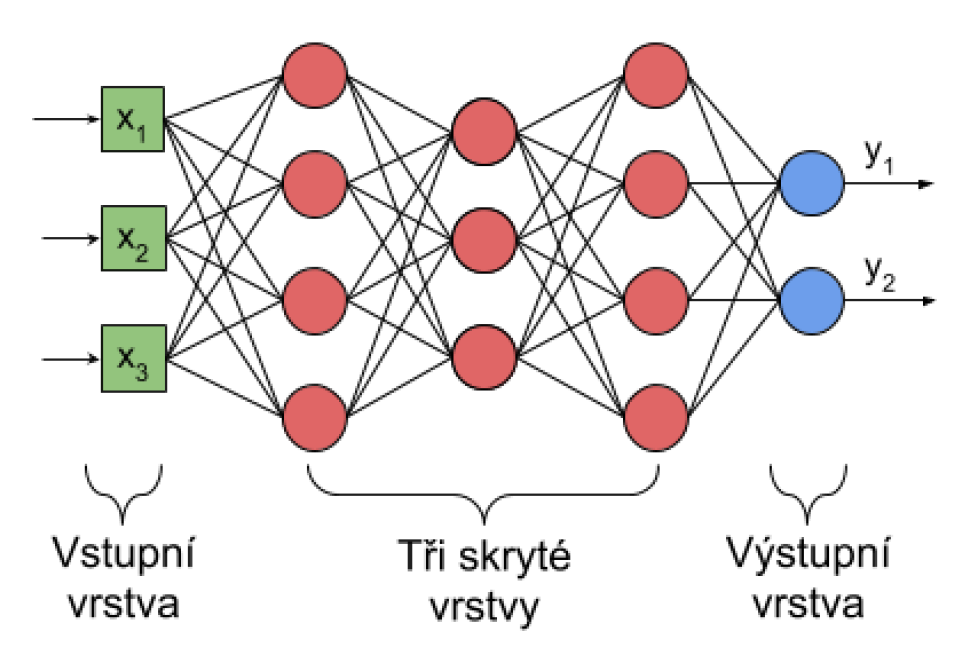
\includegraphics[width=0.5\textwidth]{Figures/layers.png}
%     \caption{Vícevrstvá, plně propojená síť \cite{lagan}}
%     \label{fig:layers}
% \end{figure}

\subsection{Proces trénování s využitím backpropagation}

Jak již bylo řečeno, proces trénování NN spočívá v nalezení optimálních hodnot
parametrů jednotlivých neuronů. Optimální parametry pak vedou k minimální
chybě. Chybou rozumíme rozdíl mezi skutečným výstupem sítě a očekávaným
výstupem. K tomu se nejčastěji používá algoritmus backpropagation (také
algoritmus zpětného šíření chyby). Nyní bude vysvětleno, jak trénování sítě
pomocí tohoto algoritmu funguje v dopředné neuronové síti. Tento algoritmus je
nicméně využíván i ve většině jiných architektur, jako jsou konvoluční či
rekurentní neuronové sítě, které budou později v této práci také využity.

Nejprve se ze vstupních dat vypočítají pomocí aktuálních parametrů sítě reálné
výstupy sítě. Tento proces se nazývá dopředný průchod (ang. forward pass).
Následně se pomocí chybové funkce (také nákladová funkce – ang. loss function)
spočítá chyba sítě. Ta vyjadřuje, v jaké míře se skutečné výstupy liší od
očekávaných. Můžou být použity různé chybové funkce, v závislosti na typu
úlohy, kterou síť řeší.

V klasifikačních úlohách je nejčastěji používaná chybová funkce křížové
entropie \cite{crossentropy}, která porovnává rozdělení pravděpodobnosti
skutečného výstupu sítě s očekávaným rozdělením pravděpodobnosti. Pro regresní
úlohy se používá například střední kvadratická chyba (ang. mean squared error –
MSE) \cite{mse} vyjadřující střední hodnotu druhých mocnin rozdílů mezi
skutečnými a očekávanými hodnotami.
% Další
% možností je absolutní chyba (ang. mean absolute error – MAE), která vyjadřuje
% střední hodnotu absolutních hodnot rozdílů.

Dále je používána metoda gradientního sestupu, která slouží k nalezení minima chybové
funkce. Za tímto účelem se vypočítají derivace chyby podle jednotlivých
parametrů sítě. Tyto derivace pak určují, jakým směrem a jak rychle se mají
dané parametry měnit, aby se chyba minimalizovala. Jelikož se derivace
parametrů v dané vrstvě vypočítávají pomocí řetězového pravidla derivací (ang.
chain rule) podle derivací parametrů následující vrstvy, je tento proces
nazýván zpětný průchod (ang. backward pass).

Jednotlivé parametry se pak podle vypočítaných derivací upraví. Velikost změny
je určená hyperparametrem rychlostí učení (ang. learning rate, také krok),
který určuje, jak rychle se mají parametry měnit. Vypočítaná derivace se
vynásobí rychlostí učení a přičte k původní hodnotě parametru. Tento proces se
opakuje pro všechny parametry sítě. Metoda gradientního sestupu umožňuje větší
změny parametrů, když jsou daleko od minima – absolutní hodnoty derivací jsou
větší, a naopak menší změny, když se k němu blíží – derivace se blíží nule.

Proces trénování sítě se skládá z opakování dopředného a zpětného průchodu pro
všechna trénovací data (někdy postupně pro jejich podmnožiny – dávky, ang.
batches). Po každém průchodu (někdy také epocha) se upraví parametry sítě podle
vypočítaných derivací. Tento proces se opakuje, dokud chyba nespadne na
požadovanou úroveň, nenastane její konvergence nebo není překročen maximální
počet iterací.

\subsection{Optimalizace procesu trénování}

V základní verzi algoritmu backpropagation se využívá výše popsaný gradientní
sestup. Ten ale může mít některé problémy, které mohou zpomalit proces
trénování nebo jej někdy zcela znemožnit. Nyní tedy budou popsány některé z
těchto problémů a jejich možná řešení.

Jedním z podstatných problémů gradientního sestupu je, že se může lehce
zaseknout v lokálním minimu, kde je derivace nulová. To může způsobit, že se
síť zastaví v nějakém suboptimálním bodě a nepokračuje do globálního minima,
které by odpovídalo optimálnímu řešení. Tento problém se často řeší přidáním
tzv. momentu do úpravy parametrů. Tento proces bere v úvahu i předchozí změny
parametrů. V případě, že se derivace parametru v průběhu trénování změní,
moment umožňuje parametrům ještě nějakou dobu pokračovat v pohybu ve stejném
směru. To většinou pomůže překonat lokální minima a dosáhnout tak globálního
minima.

Dalším řešením tohoto problému je využití stochastické aproximace gradientního
sestupu (ang. stochastic gradient descent – SGD), kde se gradient počítá pro
náhodně vybrané podmnožiny trénovacích dat. Tento postup umožňuje rychlejší
konvergenci, gradient je totiž počítán jen pro část dat, zároveň zabraňuje
zaseknutí v lokálním minimu zavedením šumu do procesu trénování. Tato metoda se
využívá nejčastěji pro velké datasety.

Dalším problémem může být nastavení optimálního kroku učení. Pokud je krok
příliš velký, může dojít k příliš velké změně, která opomine minimum, může se
tak stát, že nikdy nedosáhneme konvergence. Naopak, pokud je krok příliš malý,
může trénování trvat příliš dlouho. Řešením může být například adaptivní
nastavení kroku. Nejznámější taková metoda je RMSProp (ang. root mean square
propagation), která upravuje krok učení pro každý parametr podle průměrného
druhého momentu gradientu \cite{RMSProp}. Další možností je v průběhu trénování
postupně snižovat krok (ang. learning rate decay).

Populárním řešením těchto problémů je také Adam (ang. adaptive moment
estimation, v překladu adaptivní odhad momentu), který kombinuje zavedení
momentu a adaptivního nastavení kroku pomocí RMSProp \cite{adam}.

Další metodou, jak optimalizovat nastavení kroku, je normalizace dat mezi
vrstvami sítě (ang. batch normalization) \cite{batchnorm}. Tím se zamezí příliš
velkým změnám v jednotlivých vrstvách, které někdy destabilizují proces
trénování.

U trénování hlubokých sítí se často naráží rovněž na problém přetrénování (také
nadměrné přizpůsobení, ang. overfitting). Přetrénování nastává, když se síť
dobře naučí trénovací data, zároveň ale postrádá schopnost generalizace, a když
pak dostane nová data, nedosahuje dobrých výsledků. Nejčastěji k problému
dochází v situacích, když jsou trénovány hluboké a komplexní modely, aniž by
bylo k tomu k dispozici dostatečné množství dat. K základním řešením tohoto
problému tedy patří použití většího množství trénovacích dat – pokud jsou
dostupná, jinak se někdy zavádí umělé variace dat jako rotace či převrácení,
jinak je třeba někdy zvážit zjednodušení architektury modelu. Dále pak jsou
využívány techniky regularizace, které upravují samotný proces trénování.

Nejjednodušší regularizační technikou je tzv. předčasné zastavení, tedy
zastavení trénování v případě, že se chyba na validačních datech začne
zvyšovat. Další možností je dropout (také výpadek), kdy se u určitého počtu
náhodně zvolených neuronů v průběhu trénování nastaví na výstupu nula. Tím se
snižuje závislost sítě na konkrétních neuronech a zvyšuje se tak její schopnost
generalizace.

Další dvě metody, nazývané L1 a L2 regularizace, přičítají k chybové funkci
člen, který penalizuje velikost parametrů sítě. L1 regularizace (také metoda Lasso, z ang. least absolute shrinkage and selection operator) 
\cite{lasso} přičítá k
chybové funkci součet absolutních hodnot všech parametrů sítě vynásobený
hyperparametrem, který určuje míru této penalizace. Tato metoda vede k řídké
síti, ve které je mnoho parametrů nulových. L2 regularizace (také weight decay)
přičítá k chybové funkci součet druhých mocnin všech parametrů sítě vynásobený
hyperparametrem $\lambda$ \cite{l2}. Tato metoda vede jednak k menší
variabilitě parametrů, jednak k pomalejším změnám parametrů v průběhu  
trénování, v důsledku pak k menší citlivosti na šum v datech. Využívá se
zejména v hlubokých sítích.

\endinput
\chapter{Konvoluční neuronové sítě}
\label{sec:CNN}

I když byly jedny z prvních NN použity ke zpracování obrazu, brzy se ukázalo,
že pro zpracování obrazu s větším rozlišením a větším množstvím kanálů je
klasická architektura NN velmi neefektivní. Bylo tedy třeba vytvořit jinou
architekturu, která by efektivně zpracovávala obrazová data. Nejznámější
takovou architekturou je konvoluční neuronová síť (ang. convolutional neural
network - CNN), která bude popsána v této kapitole.

\section{Problémy zpracování obrazu pomocí klasických neuronových sítí}

Klasickým přístupem pro zpracování obrazů pomocí neuronové sítě je vytvoření
sítě se stejným počtem prvků vstupní vrstvy, jako je počet pixelů vstupního
obrazu (za předpokladu jednoho kanálu). Tato vrstva je pak plně propojena s
několika skrytými vrstvami, výstupní vrstva pak buď vrací kategorie, v případě
klasifikace, nebo hodnoty hledaných atributů, jako je lokalizace objektů či
souřadnice klíčových bodů, v případě regrese.

Problémem tohoto přístupu je rozměr vstupních dat takové sítě. Běžná velikost
obrazu v dnešní době dosahuje několika miliónů pixelů, tento počet je ale ještě
vynásoben počtem kanálů, většinou třemi (RGB). To znamená, že velikost vstupní
vrstvy sítě je velmi vysoká, a aby byla taková síť efektivní, musí mít větší
počet skrytých vrstev a neuronů v těchto vrstvách. Ve výsledku má taková síť
velký počet parametrů, které je třeba natrénovat. Trénování takové sítě je
možné, je ale velmi nepraktické. Bylo by potřeba velké množství trénovacích
dat, jinak by s velkou pravděpodobností došlo k přetrénování sítě. I kdyby ale
bylo k dispozici dostatečné množství trénovacích dat, bylo by jak trénování,
tak i používání sítě velmi výpočetně i paměťově náročné.

CNN se proto tento problém řeší tak, že se snaží zredukovat rozměr vstupních
dat pomocí konvolučních vrstev, které jsou schopny efektivně zpracovávat
obrazová data.

\section{Konvoluce}

V kontextu počítačové grafiky je konvoluce binární operace, kdy pro daný pixel
sečteme hodnoty pixelů v jeho okolí vynásobené váhami vyjádřenými maskou, která
se nazývá jádro konvoluce (ang. kernel). Výsledný obraz je taky nazýván
konvoluce. Z matematického pohledu se jedná o diskrétní dvourozměrnou konvoluci
- binární operaci diskrétních funkcí, která je definována následovně:

\begin{equation*}
    (h*f)(x,y)=\sum _{i=-k}^{k}\sum _{j=-k}^{k}h(x-i,y-j)\cdot f(i,j)
\end{equation*}

kde $h$ je vstupní obraz, $f$ je jádro konvoluce, velikost jádra je $2k+1
    \times 2k+1$, a $x$ a $y$ jsou souřadnice pixelu, ke kterému se jádro aplikuje.

Hodnota konvoluce na dané pozici je tedy suma součinů hodnot pixelů vstupního
obrazu a hodnot váh vyjádřených jádrem konvoluce položeným středem na danou
pozici, viz obrázek \ref{fig:convolution}. Nejčastěji je velikost jádra lichá,
jelikož je pak jednodušší určení středu jádra.

\begin{figure}[]
    \centering
    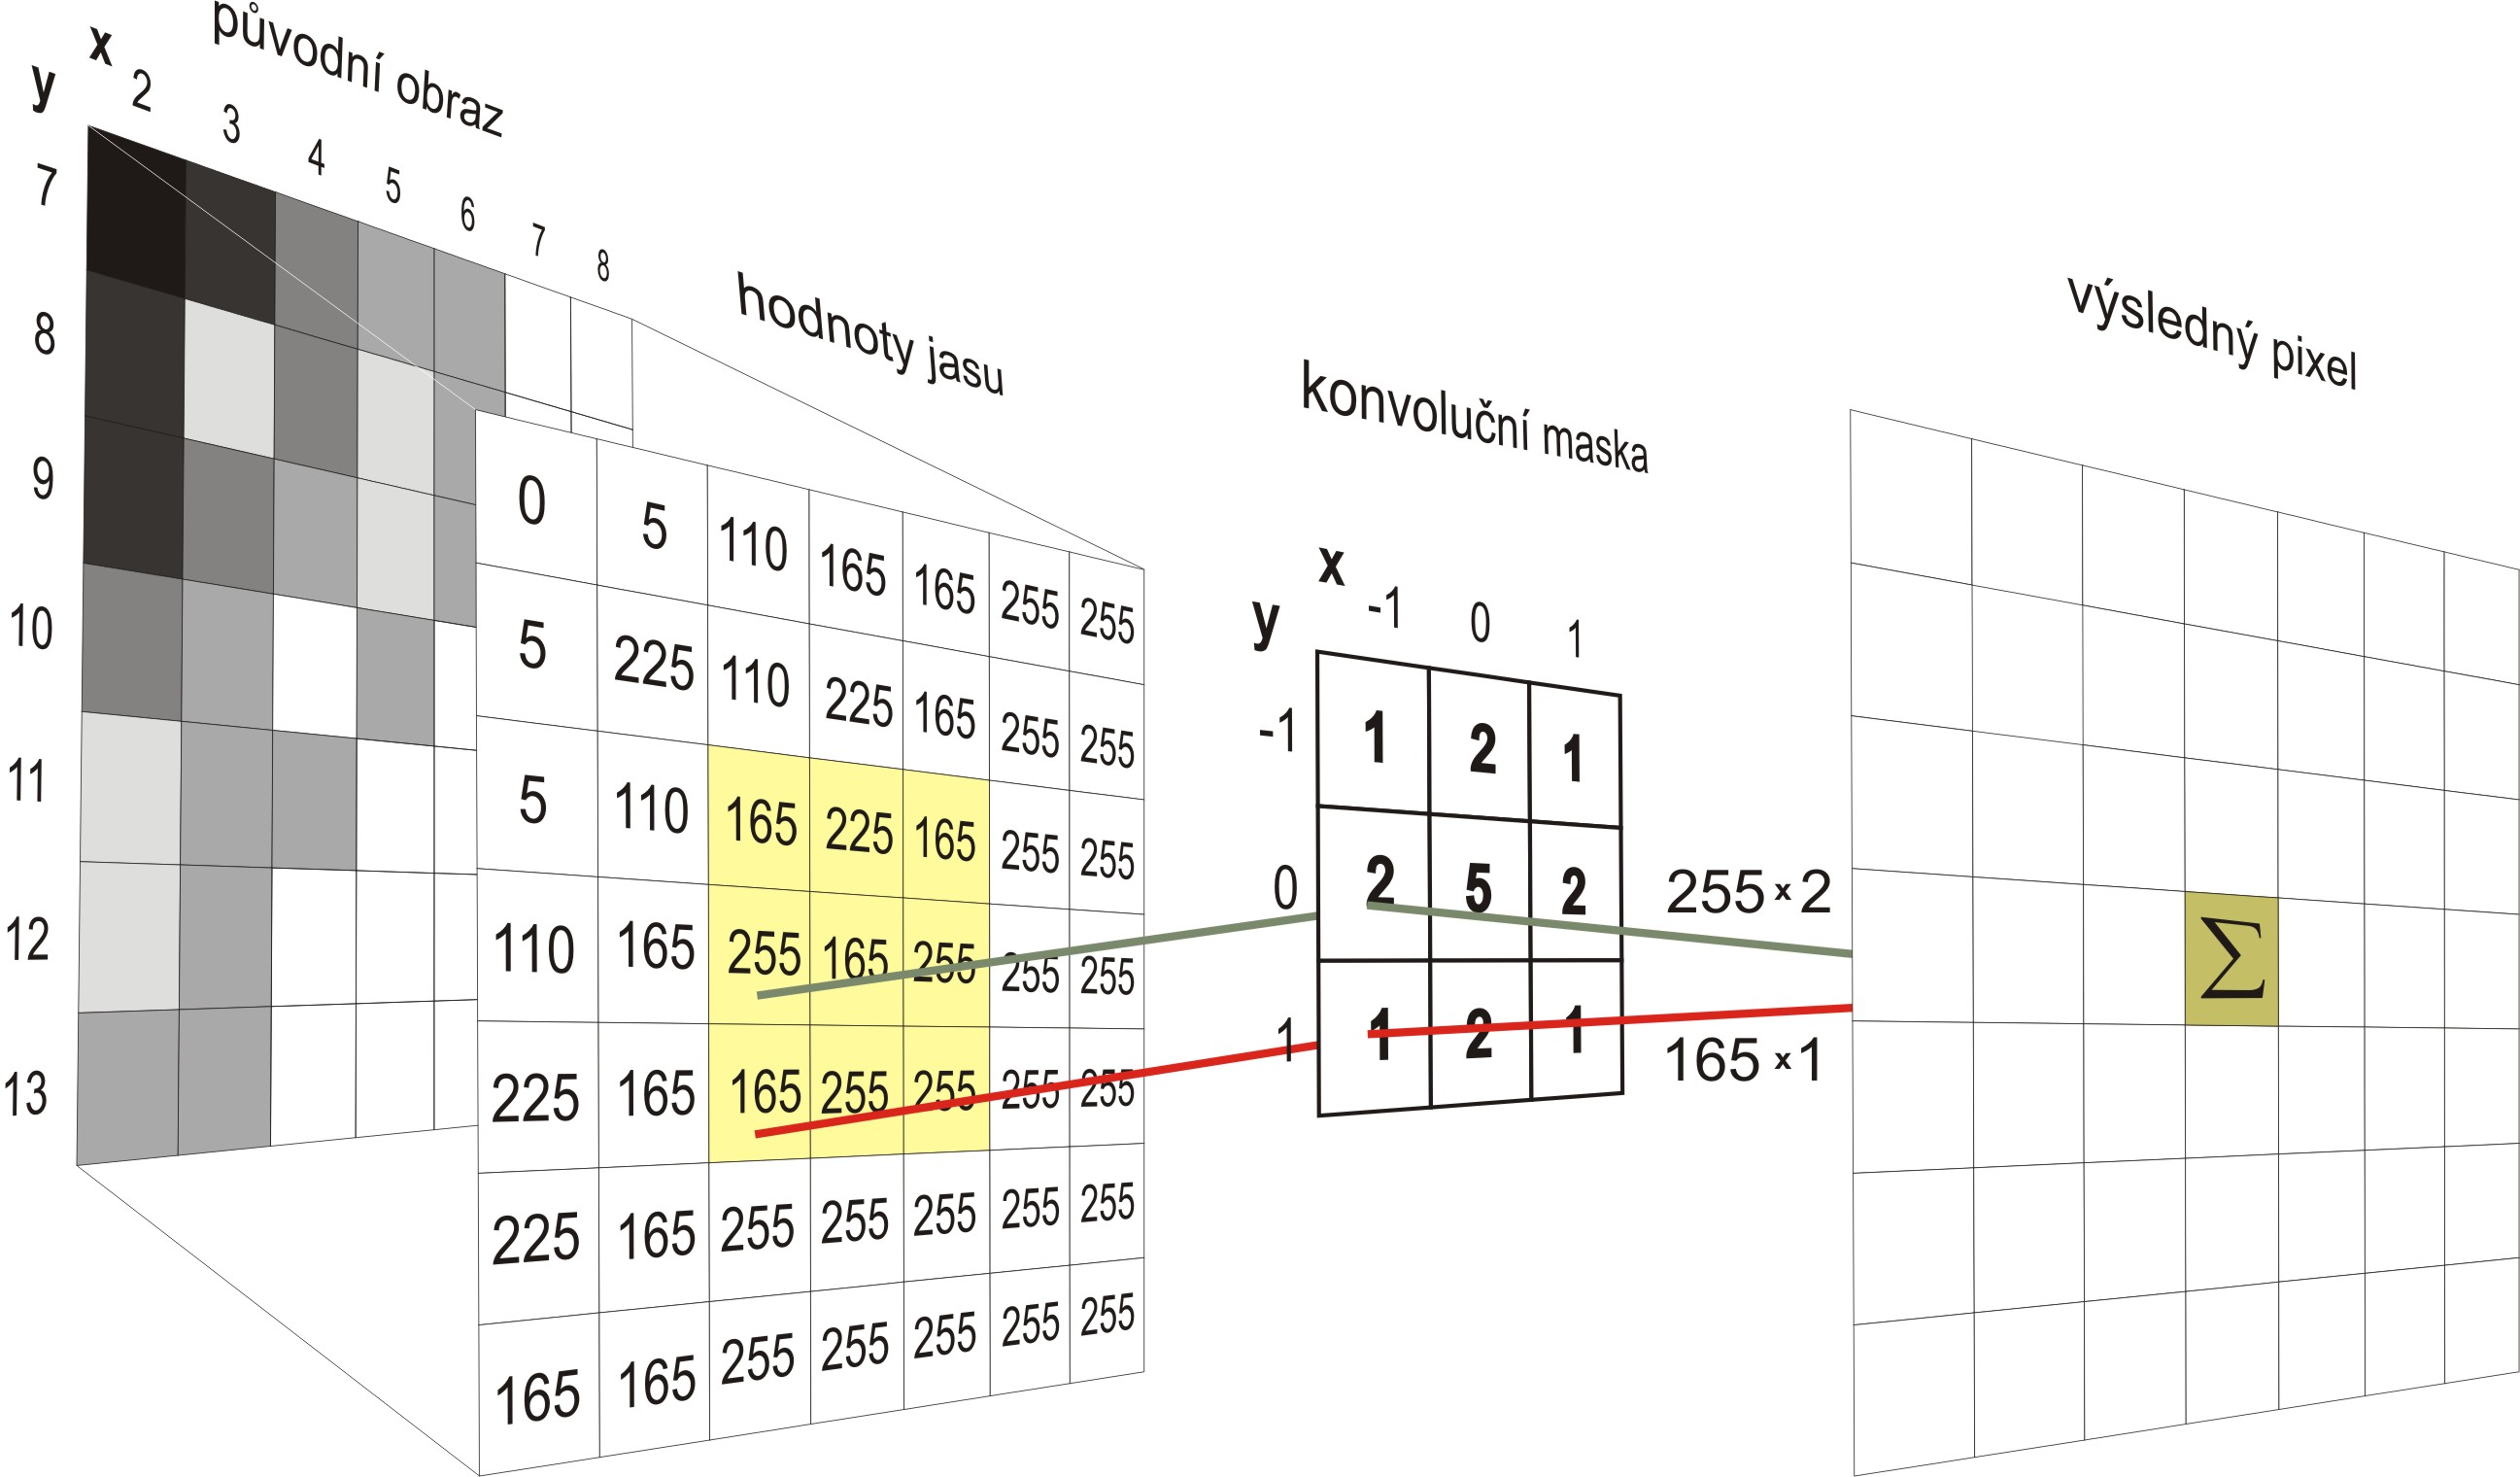
\includegraphics[width=0.8\textwidth]{Figures/convolution.jpg}
    \caption{Princip diskrétní dvourozměrné konvoluce \cite{}}
    \label{fig:convolution}
\end{figure}

Konvoluce je velmi rozšířená operace v počítačové grafice a zpracování obrazu,
k nejpoužívanějším aplikacím patří například rozmazání nebo detekce hran.

Pro rozmazání se používá například průměrovací filtr (ang. box blur)
využívající jádro, které má na všech pozicích hodnotu $1/n$, kde $n$ je počet
prvků jádra, viz obrázek \ref{fig:blur}. Výsledná hodnota konvoluce daného
pixelu je tedy rovná průměru hodnot tohoto pixelu a jeho sousedů. Dalším často
využívaným filtrem je Gaussovo rozostření, viz obrázek \ref{fig:blur}. Rozmazání
je někdy využíváno v počítačovém vidění jako první krok, za účelem odstranění
šumu z obrazu.

Pro detekci hran se často používá Sobelův operátor, který využívá dvě jádra -
pro vertikální a horizontální hrany. Jádra pro detekci hran jsou zobrazena na
obrázku \ref{fig:sobel}.

\begin{figure}[]
    \centering
    \begin{equation*}
        {\displaystyle {\frac {1}{9}}{
                \begin{bmatrix}
                    1 & 1 & 1 \\
                    1 & 1 & 1 \\
                    1 & 1 & 1 \\
                \end{bmatrix}},\ \ \ \ }
        {\displaystyle {\frac {1}{16}}{
                \begin{bmatrix}
                    1 & 2 & 1 \\
                    2 & 4 & 2 \\
                    1 & 2 & 1 \\
                \end{bmatrix}}}
    \end{equation*}

    \caption{Jádro konvoluce pro průměrovací a Gaussovo rozostření}
    \label{fig:blur}
\end{figure}
\begin{figure}[]
    \centering
    \begin{equation*}
        {\displaystyle {
                \begin{bmatrix}
                    -1 & 0 & 1 \\
                    -2 & 0 & 2 \\
                    -1 & 0 & 1 \\
                \end{bmatrix}},\ \ \ \ }
        {\displaystyle {
                \begin{bmatrix}
                    -1 & -2 & -1 \\
                    0  & 0  & 0  \\
                    1  & 2  & 1  \\
                \end{bmatrix}},\ \ \ \ }
    \end{equation*}

    \caption{Jádro konvoluce pro detekci vertikálních a horizontálních hran využívané pro Sobelův operátor}
    \label{fig:sobel}
\end{figure}

V případě více kanálů vstupního obrazu musí být připraveno zvlášť jádro pro
každý kanál. Výsledné konvoluce se pak sečtou. Můžeme se na tuto situaci dívat
i jako na třírozměrné konvoluční jádro s rozměrem třetí dimenze rovným počtu
kanálů vstupního obrazu. Konvoluce je pak prováděná tak, že na každé pozici
vstupního obrazu provedeme součet vah jádra vynásobených hodnotami vstupního
obrazu na příslušných pozicích napříč všemi kanály. Výstup takové konvoluce má
pouze jeden kanál.

Myšlenkou konvolučních neuronových sítí je nahradit plně propojené vrstvy
konvolučními vrstvami. Ruční nastavení všech hodnot jader tak, aby konvoluční
vrstvy extrahovaly požadované vlastnosti z obrázku, je ale velmi obtížné, v
případě složitějších či obecnějších problémů téměř nemožné. V 1989 proto Yann
LeCun et al. navrhli metodu, jak se síť může hodnoty jader naučit sama, a tak
si efektivně vytvořit i složitější filtry, které by člověk těžko navrhl ručně.
Zjistili, že váhy konvolučních jader se mohou trénovat pomocí algoritmu
backpropagation stejně jako váhy neuronů v plně propojených vrstvách.

Takový přístup má mnoho výhod. Konvoluce se dá velmi dobře paralelizovat a
zajistit tak vysokou efektivitu výpočtů. Oproti plně propojeným vrstvám má vždy
konvoluce s jedním jádrem počet vah pouze rovný velikosti jádra. I v případě
provedení mnoha konvolucí je počet výrazně menší než v případě potřebného počtu
a velikosti plně propojených vrstev. Zároveň lze pomocí konvolucí efektivně
extrahovat různé vlastnosti ze vstupního obrazu, ty pak pomocí plně propojených
vrstev zpracovat a využít k řešení problému. Proto se taky výstupu konvoluce
často říká mapa příznaků (ang. feature map).

\section{Krok a padding}

Pro pochopení funkčnosti konvolučních neuronových sítí je ještě důležité
pochopit dva parametry, které ovlivňují výstup konvoluční vrstvy. Jedná se o
krok (ang. stride) a padding (česky vycpávka či doplnění).

Krok určuje, co kolik pixelů se aplikuje jádro konvoluce na vstupní obraz.
Pokud tedy bude krok $k = 1$, bude jádro aplikováno na každý pixel vstupního
obrazu. Pokud bude krok $k = 2$, bude jádro aplikováno na každý druhý pixel
vstupního obrazu. Pokud bude krok $k > 1$, bude výstup konvoluce násobně menší.

Jelikož na nejkrajnější pixely nemůžeme aplikovat jádro, protože by přesahovalo
hranice obrazu, bude se obraz z každou konvolucí nežádaně zmenšovat i při
jednotkovém kroku. Pokud použijeme například jádro o velikosti $3 \times 3$,
bude výsledná mapa o 2 řádky a 2 sloupce menší, než byl vstupní obraz. Dalším
problémem je, že ve výsledné konvoluci je marginalizován vliv krajních pixelů.
Obraz je tedy jistým způsobem oříznut. Tyto problémy se proto někdy řeší pomocí
tzv. paddingu. Je to technika, kdy se vstupní obraz rozšíří o takový počet
pixelů z každé strany, aby vzhledem k velikosti konvolučního jádra bylo možné
aplikovat jádro i na krajní pixely obrazu.

Velikost výstupní mapy konvoluce je tedy dána vztahem:

\begin{equation*}
    \left\lfloor \frac{n+2p-f}{s}+1 \right\rfloor \times \left\lfloor \frac{n+2p-f}{s}+1 \right\rfloor
\end{equation*}

kde $n$ je velikost vstupního obrazu, $p$ je velikost paddingu, $s$ je krok a
jádro je velikosti $f \times f$.

\section{Konvoluční vrstva}

Konvoluční vrstva je základním prvkem konvoluční neuronové sítě. V jistém slova
smyslu je podobná plně propojené vrstvě, jelikož obsahuje váhy, biasy a
aktivační funkce. Namísto plného propojení s neurony následující vrstvy je ale
aplikována konvoluce na vstupní data. K výstupní mapě je přičten bias a
následně může být aplikována aktivační funkce.

Jedná vrstva může mít několik konvolučních jader, každé s vlastními váhami a
biasem. Je třeba zároveň pamatovat, že každé jádro musí mít hloubku rovnou
počtu vstupních map, resp. počtu kanálu vstupního obrazu v případě vstupní
vrstvy. Konvoluci pak aplikujeme zvlášť pro každé jádro, počet výstupních map
příznaků tedy bude roven počtu jader v dané vrstvě. V praxi bude každé jádro
vyjadřovat jinou vlastnost, kterou se snažíme ze vstupního obrazu extrahovat.

Množinu parametrů dané konvoluční vrstvy tedy tvoří hodnoty jader a jejích
příslušné biasy. K hyperparametrům pak patří počet jader a jejich velikost,
aktivační funkce, krok a padding.

\section{Poolovací vrstva}
Jak již bylo zmíněno, v konvolučních vrstvách vzniká vícero map příznaků
vyjadřující různé vlastnosti. Tím se ale množství dat zvětšuje, což porušuje
samotnou myšlenku konvolučních sítí, která je založena na snaze zredukovat
rozměr dat. Proto se snažíme rozměr map příznaků zmenšovat. Jak již bylo
zmíněno, dojde k redukci rozměrů v konvoluční vrstvě, pokud použijeme krok $k >
    1$. Častěji ale je k tomuto účelu prováděno podvzorkování dat v tzv.
poolovacích vrstvách (z ang. pooling layer).

V poolovací vrstvě je vstupní mapa rozdělená do stejně velkých čtvercových
oblastí velikosti $t \times t$, na základě hodnot v daném čtverci je pak
vytvořen jeden pixel výstupní mapy. K nejčastěji používaným metodám patří
max-pooling a average-pooling. Max-pooling vybere z dané oblasti největší
hodnotu, zatímco average-pooling vyhodnotí z každé oblasti průměr hodnot.
Velikost výstupní mapy pro vstup velikosti $n \times n$ a poolovací oblasti
velikosti $t \times t$ je tedy $\left\lfloor \frac{n}{t} \right\rfloor \times
    \left\lfloor \frac{n}{t} \right\rfloor$.

\section{Architektura CNN}

Konvoluční neuronové sítě se skládají ze dvou částí - konvoluční části a plně
propojené části.

Konvoluční část se skládá z několika konvolučních vrstev proplétaných s
poolovacími vrstvami. V této části se pracuje s mapami příznaků. Její výstupem
je soubor map příznaků, který vyjadřuje různé vlastnosti vstupního obrazu.

Plně propojená část je pak klasická dopředná neuronová síť, která na základě
extrahovaných vlastností provádí klasifikační či regresní úlohu. Před vstupem
do plně propojené části jsou mapy příznaků převedené do jednoho vektoru o
velikosti rovné součtu velikostí všech map příznaků.

\endinput

\chapter{Rekurentní neuronové sítě}
\label{chap:RNN}

Rekurentní neuronové sítě (ang. Recurrent Neural Networks – RNN) je kategorie
neuronových sítí, které do své architektury zapojují zpětnou vazbu. Na rozdíl
od dopředných sítí, které zpracovávají jednotlivé vstupy nezávisle, rekurentní
sítě spolu s aktuálním vstupem při evaluaci zohledňují nějakým způsobem i
výsledek předchozí iterace. Jejich využití tedy je ve dvou oblastech: analýza
změn pozorovaného objektu v čase (např. sledování pohybu, analýza chování či
predikce časových řad) a zpracování kontextuálních informací jako je např.
přirozený jazyk.

Jelikož v případě pádu se nejedná o statickou informaci, ale o jistý druh
pohybu, mohly by právě rekurentní sítě stanovit optimální cestu pro naše řešení
\cite{dhruv2020image}. Pojďme se tedy nyní podívat na to, jak rekurentní
neuronové sítě fungují a jaké jsou jejich nejpoužívanější architektury.

\section{Základní principy}

Data, která v aktuální iteraci přebíráme z předchozí iterace, se často označují
jako skrytý stav (ang. hidden state). Je to forma paměti, která se s každou
iterací aktualizuje. Často je reprezentován jako stavová vrstva (ang. state
layer nebo context layer), která přijímá hodnoty z výstupu neuronů, uchovává je
mezi iteracemi a předává je spolu se vstupními daty na vstup neuronů. Na
obrázku \ref{fig:rnn} je tato vrstva reprezentována neurony $c_i$.

Nejjednodušší forma rekurentní neuronové sítě je NN s jednou skrytou vrstvou;
tato vrstva kromě dat ze vstupní vrstvy přijímá také výstup předchozí iterace
svých vlastních neuronů. Příklady takových sítí jsou Elmanova a Jordanova síť
\cite{elman} \cite{jordan}, které byly prvními rekurentními sítěmi
využívajícími backpropagation pro trénování.
% buď svých vlastních neuronů, anebo z neuronů výstupní vrstvy, viz obrázek
% \ref{fig:rnn}. Obrázek je zjednodušený, v praxi jsou stavová a skrytá vrstva
% plně propojeny. Tyto architektury se jmenují Elmanova síť \cite{elman}, resp.
% Jordanova síť \cite{jordan}, od jejích tvůrců. Tyto sítě jsou také známé jako
% jednoduché rekurentní sítě (ang. Simple Recurrent Networks – SRN).

% I když pojem rekurentních sítí byl známý už od začátků neuronových sítí jako
% takových a byly i případy jejích použití, právě tyto sítě patřily k prvním,
% které používaly pro trénování algoritmus backpropagation. Jednoduché rekurentní
% sítě uchovávají pouze krátkodobé vzory a jsou vhodné spíše pro jednoduché
% úlohy, jako je např. predikce časových řad.

% \begin{figure}[]
%     \centering
%     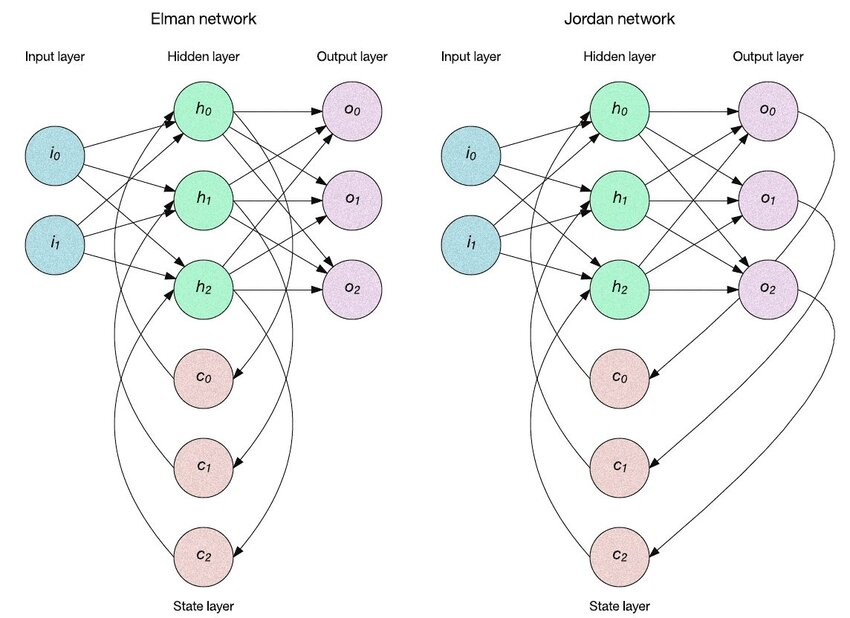
\includegraphics[width=0.8\textwidth]{Figures/rnn.png}
%     \caption{Základní architektury RNN \cite{aksoy}}
%     \label{fig:rnn}
% \end{figure}

\subsection{Hluboké rekurentní sítě}

Stejně jako u dopředných neuronových sítí, kde se od jednoduchého perceptronu
přešlo k hlubokým sítím, se i rekurentní sítě rozšířily na více vrstev. V
hlubokých rekurentních neuronových sítích (ang. deep RNN – DRNN) jsou pak
jednotlivé vrstvy většinou podobné struktuře Elmanovy sítě \cite{elman} -
zpětná vazba je předávána pouze v rámci jedné vrstvy, nikoliv mezi vrstvami RNN
(například z výstupní vrstvy do první skryté vrstvy) \cite{deeprnn}. Má to
několik důvodů. Trénování sítě se zpětnou vazbou mezi vrstvami by bylo velmi
složité a obtížné. Také, u neuronových sítí obecně platí, že každá vrstva sítě
se učí pochopit problém na jiné úrovni abstrakce, zpětná vazba přes několik
vrstev by pak mohla narušit stabilitu tohoto procesu a omezit kvalitu učení.

\subsection{Trénování rekurentních sítí}

Pro pochopení rekurentních neuronových sítí je třeba si vysvětlit, jak se
trénují. Pro vizualizaci trénování RNN se tyto sítě takzvaně rozbaluje v čase
(ang. unrolling). Znamená to, že jednotlivé iterace vizualizujeme jako sekvenci
stejných sítí (stejné váhy), které v čase $t$ přijímají vstup $x_t$ a vracejí
výstup $y_t$, viz obrázek \ref{fig:bptt}. Zároveň místo smyček znázorňujících
zpětnou vazbu přijímá skrytá vrstva v čase $t$ stav $c_{t-1}$ z předchozí
iterace. Takto je propojená mezi iteracemi každá skrytá vrstva (na obrázku
\ref{fig:bptt} vizualizováno propojení přes stavovou vrstvu).

\begin{figure}[]
    \centering
    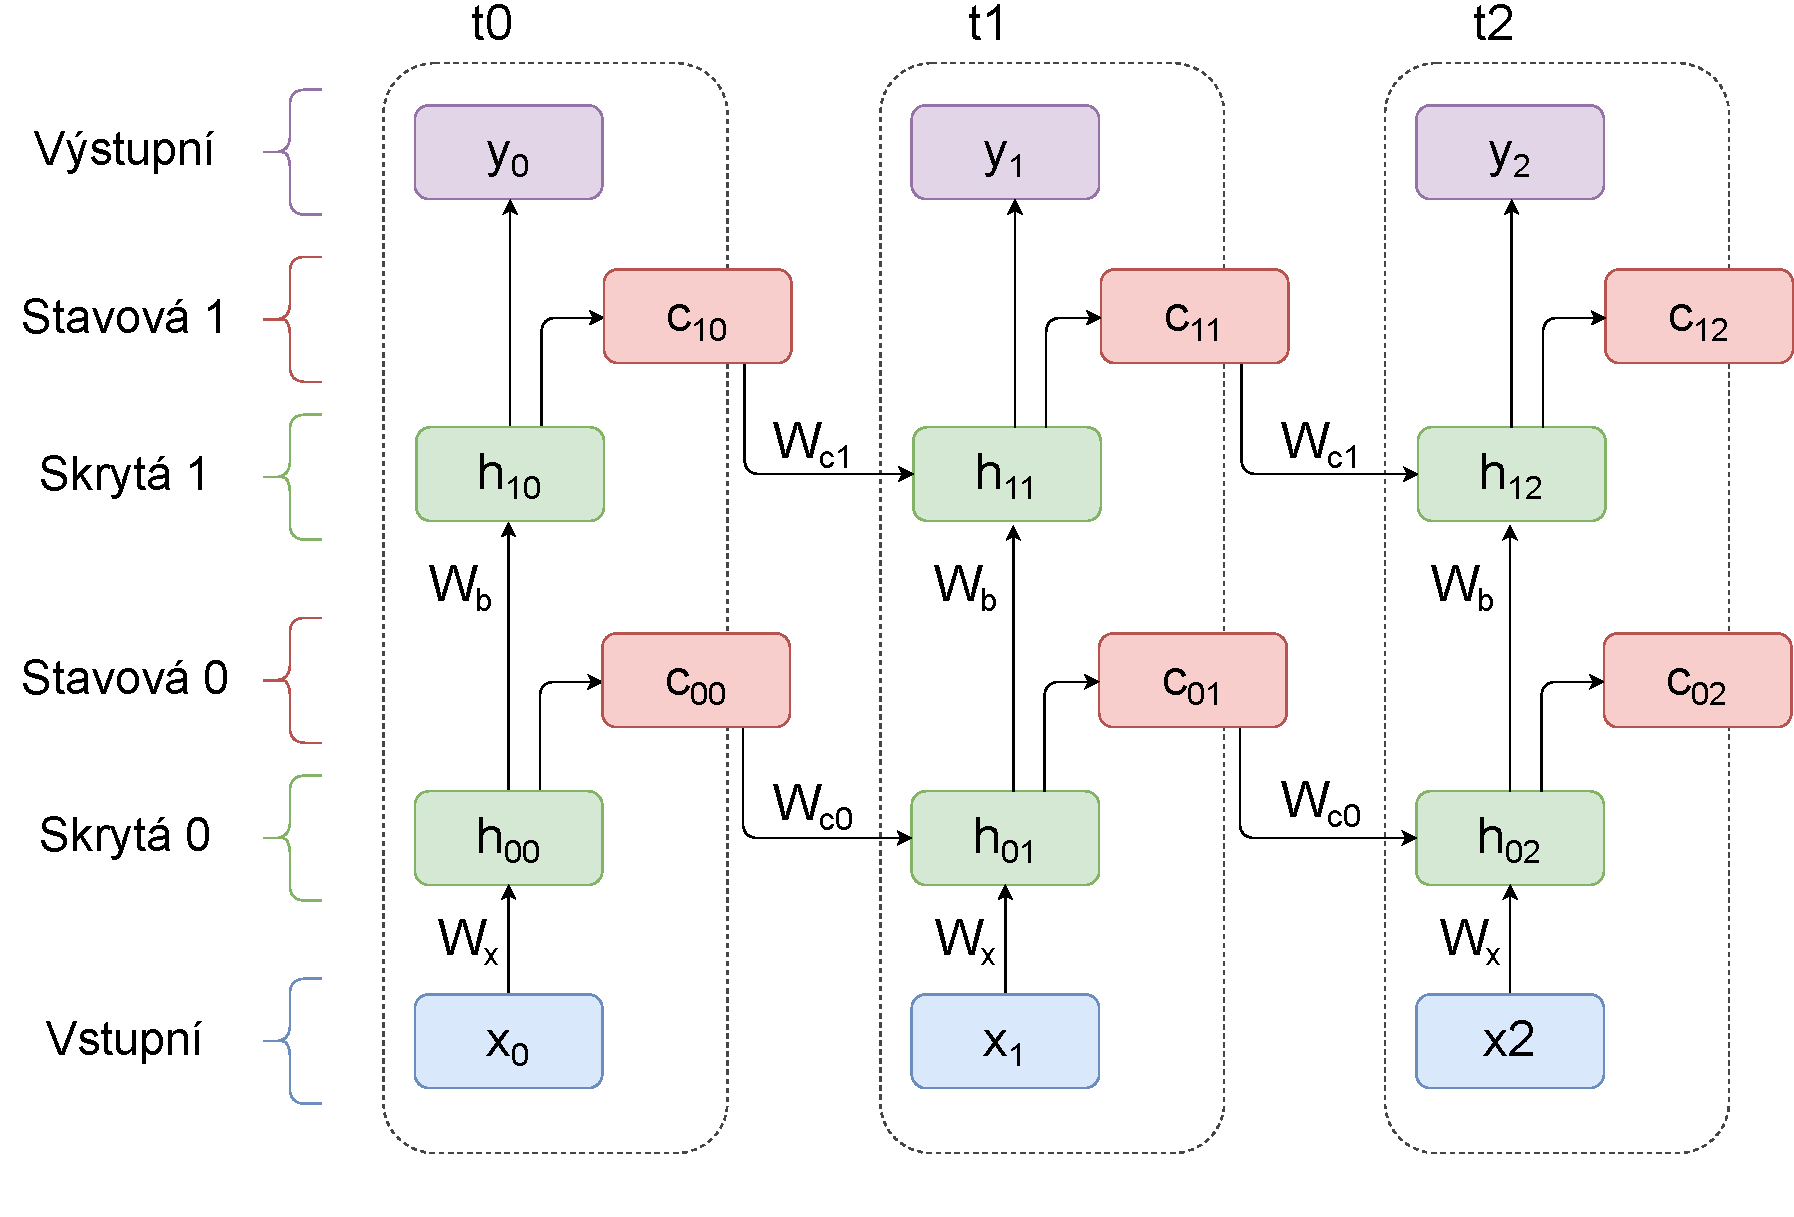
\includegraphics[width=0.75\textwidth]{Figures/BPTT.pdf}
    \caption{Unrolling hluboké RNN}
    \label{fig:bptt}
\end{figure}

Při trénování se pak používá algoritmus zpětného šíření chyby v čase (ang.
backpropagation through time – BPTT). Algoritmus funguje stejně jako klasický
backpropagation, šíří se ale nejenom vrstvami, ale i iteracemi. Unrolling nám
pomáhá backpropagation pochopit, jednotlivé iterace totiž jsou naskládány jako
vrstvy a celou síť řešíme jako klasickou dopřednou NN.

\subsection{Problémy mizejícího a explodujícího gradientu}

Výše popsané základní rekurentní neuronové sítě, někdy označovány jako vanilla
RNN, trpí několika zásadními problémy. U dopředných sítí jsme zmiňovali problém
mizejícího gradientu (ang. vanishing gradient), vystupující zejména u hlubších
sítí. Ten se projevuje i u RNN a je zesílený tím, že jsou jednotlivé iterace
naskládané na sebe, podobně jako vrstvy. Zejména pak u delších sekvencí budou
mít dřívější vstupy velmi malý vliv na učení sítě.

U RNN se také projevuje problém opačný – explodující gradient (ang. exploding
gradient). Ten způsobuje, že v průběhu sekvence se váhy začnou exponenciálně
zvětšovat a dosáhnou tak nepřiměřeně velkých hodnot.

Podívejme se, co přesně tyto problémy způsobuje. Součástí algoritmu
backpropagation je počítání parciální derivace ztrátové funkce podle
jednotlivých vah. V případě BPTT potřebujeme mimo jiné počítat parciální
derivace skrytého stavu mezi jednotlivými iteracemi $\frac{\partial
        h_{t-1}}{\partial h_t}$. Tyto derivace následně opakovaně násobíme při použití
řetězového pravidla. Pokud je tato derivace $\frac{\partial h_{t-1}}{\partial
        h_t}<1$, jeho vynásobení bude mít za následek postupné zmenšování gradientu.
Pokud budeme například mít sekvencí $100$ iteraci, pak i kdyby se gradienty v
každé iteraci zmenšovaly $0,9$ krát, po $100$ iteracích by gradient klesl na
hodnotu $0,9^{100} \approx 2,7 \times 10^{-5}$, což je prakticky nula. Pokud se
naopak bude gradient zvětšovat $1,1$ krát, po $100$ iteracích by gradient
vzrostl na $1,1^{100} \approx 13 780$, což způsobí úplnou destabilizaci sítě a
nedosáhneme žádného výsledku. Vidíme tedy, že v případě, kdy je $\frac{\partial
        h_{t-1}}{\partial h_t}>1$, dochází k explodujícímu gradientu.

Z důvodu těchto problémů byly vyvinuty složitější rekurentní struktury. Jejich
architektura je v podstatě podobná, jednotlivé vrstvy jsou ale zastoupeny
jinými stavebními bloky, které umožňují zejména širší pochopení kontextu a
efektivnější proces trénování. Vanilla RNN se v praxi dnes využívají velmi
zřídka. K nejpoužívanějším architekturám patří LSTM (ang. long short-term
memory) a GRU (ang. gated recurrent unit), které nyní popíšeme.

\section{LSTM}

Dlouhá krátkodobá paměť (ang. long short-term memory – LSTM ), představena
Hochreiterem a Schmidhuberem v roce 1997, je typ rekurentní neuronové sítě,
který byl navržen tak, aby překonal problémy mizejícího a explodujícího
gradientu.

\begin{figure}[]
    \centering
    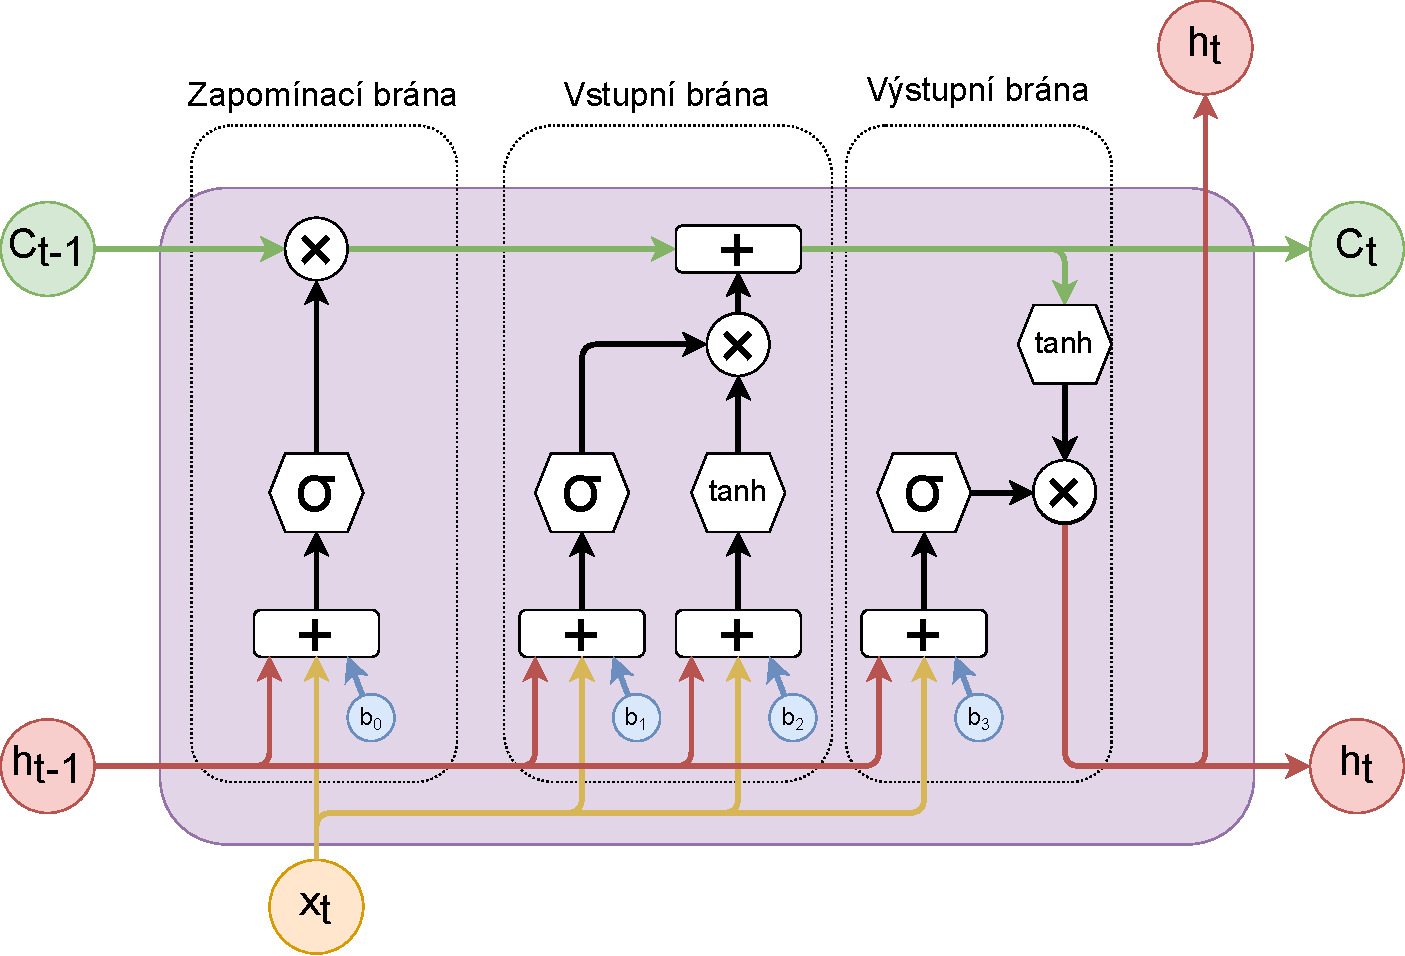
\includegraphics[width=0.7\textwidth]{Figures/LSTM_unit.pdf}
    \caption{Jednotka LSTM}
    \label{fig:lstm}
\end{figure}

Její základem je jednotka, viz obrázek \ref{fig:lstm}.1, která ve třech
stádiích aktualizuje krátkodobou a dlouhodobou paměť. Dlouhodobá paměť je
reprezentovaná pomocí stavu buňky (ang. cell state, na obrázku \ref{fig:lstm}.1
$c_t$), který je postupně upravován a nakonec předán další iteraci. Dokáže
uchovávat dlouhodobé závislosti. Krátkodobá paměť je reprezentována pomocí
skrytého stavu. Je použita pro úpravu dlouhodobé paměti, v konečném stadiu je
ale vždy v rámci dané iterace vytvořena nová. Je tak vhodná pro uchování
krátkodobých závislostí. Na obrázku \ref{fig:lstm} je znázorněna jako $h_t$.

Jednotka LSTM má tři hlavní komponenty – zapomínací bránu (ang. forget gate),
vstupní bránu (ang. input gate) a výstupní bránu (ang. output gate). Brány
určují, které informace mají být předány dál.

První, zapomínací brána určuje, které informace z dlouhodobé paměti $c_{t-1}$
se dostanou dále – co má jednotka zapomenout, resp. zapamatovat. Ve vstupní
bráně se nejprve vytvoří kandidátní stav buňky. Ten je výsledkem neuronové
vrstvy s tangenciální aktivační funkcí, do které vstupuje aktuální vstup $x_t$
a krátkodobá paměť $h_{t-1}$. Pak se určí, které informace z kandidátního stavu
buňky se přičtou do stavu buňky a vznikne tak aktuální stav buňky $c_t$. Ve
výstupní bráně se pomocí tangenciální aktivační funkce vytvoří na základě stavu
buňky $c_t$ kandidátní skrytý stav. Pak se určí, které z těchto informací budou
tvořit nový skrytý stav $h_t$.

V každé bráně tedy máme informace, pro které určujeme, zda je poslat dále či
nikoliv, nazvěme je propouštěný obsah (předchozí stav buňky, kandidátní stav
buňky či kandidátní skrytý stav). Toto určení se provádí vždy pomocí neuronové
vrstvy se sigmoidní aktivační funkcí. Do těchto vrstev vstupuje vždy předchozí
skrytý stav $h_{t-1}$ a aktuální vstup $x_t$. Výstupem je hodnota mezi $0$ a
$1$ pro každou informaci. Pak se tento výsledek vynásobí propouštěným obsahem.
Pokud je výstup této vrstvy $0$, informace se nepředávají dál, pokud je $1$,
informace se předávají dále. Vstupy do všech neuronových vrstev jsou vždy
vynásobeny váhami, ty ale nejsou pro jednoduchost na obrázku \ref{fig:lstm}.1
zobrazeny. Na obrázku \ref{fig:lstm_deep} je znázorněna rozvinutá hluboká LSTM
síť. Jednotlivé vrstvy sítě jsou naskládány vertikálně, jednotlivé iterace pak
jsou rozvinuty vedle sebe. Jednotlivé vrstvy si předávají skrytý stav -
krátkodobou paměť, mezi iteracemi si pak daná vrstva předává krátkodobou i
dlouhodobou paměť.

\begin{figure}
    \centering
    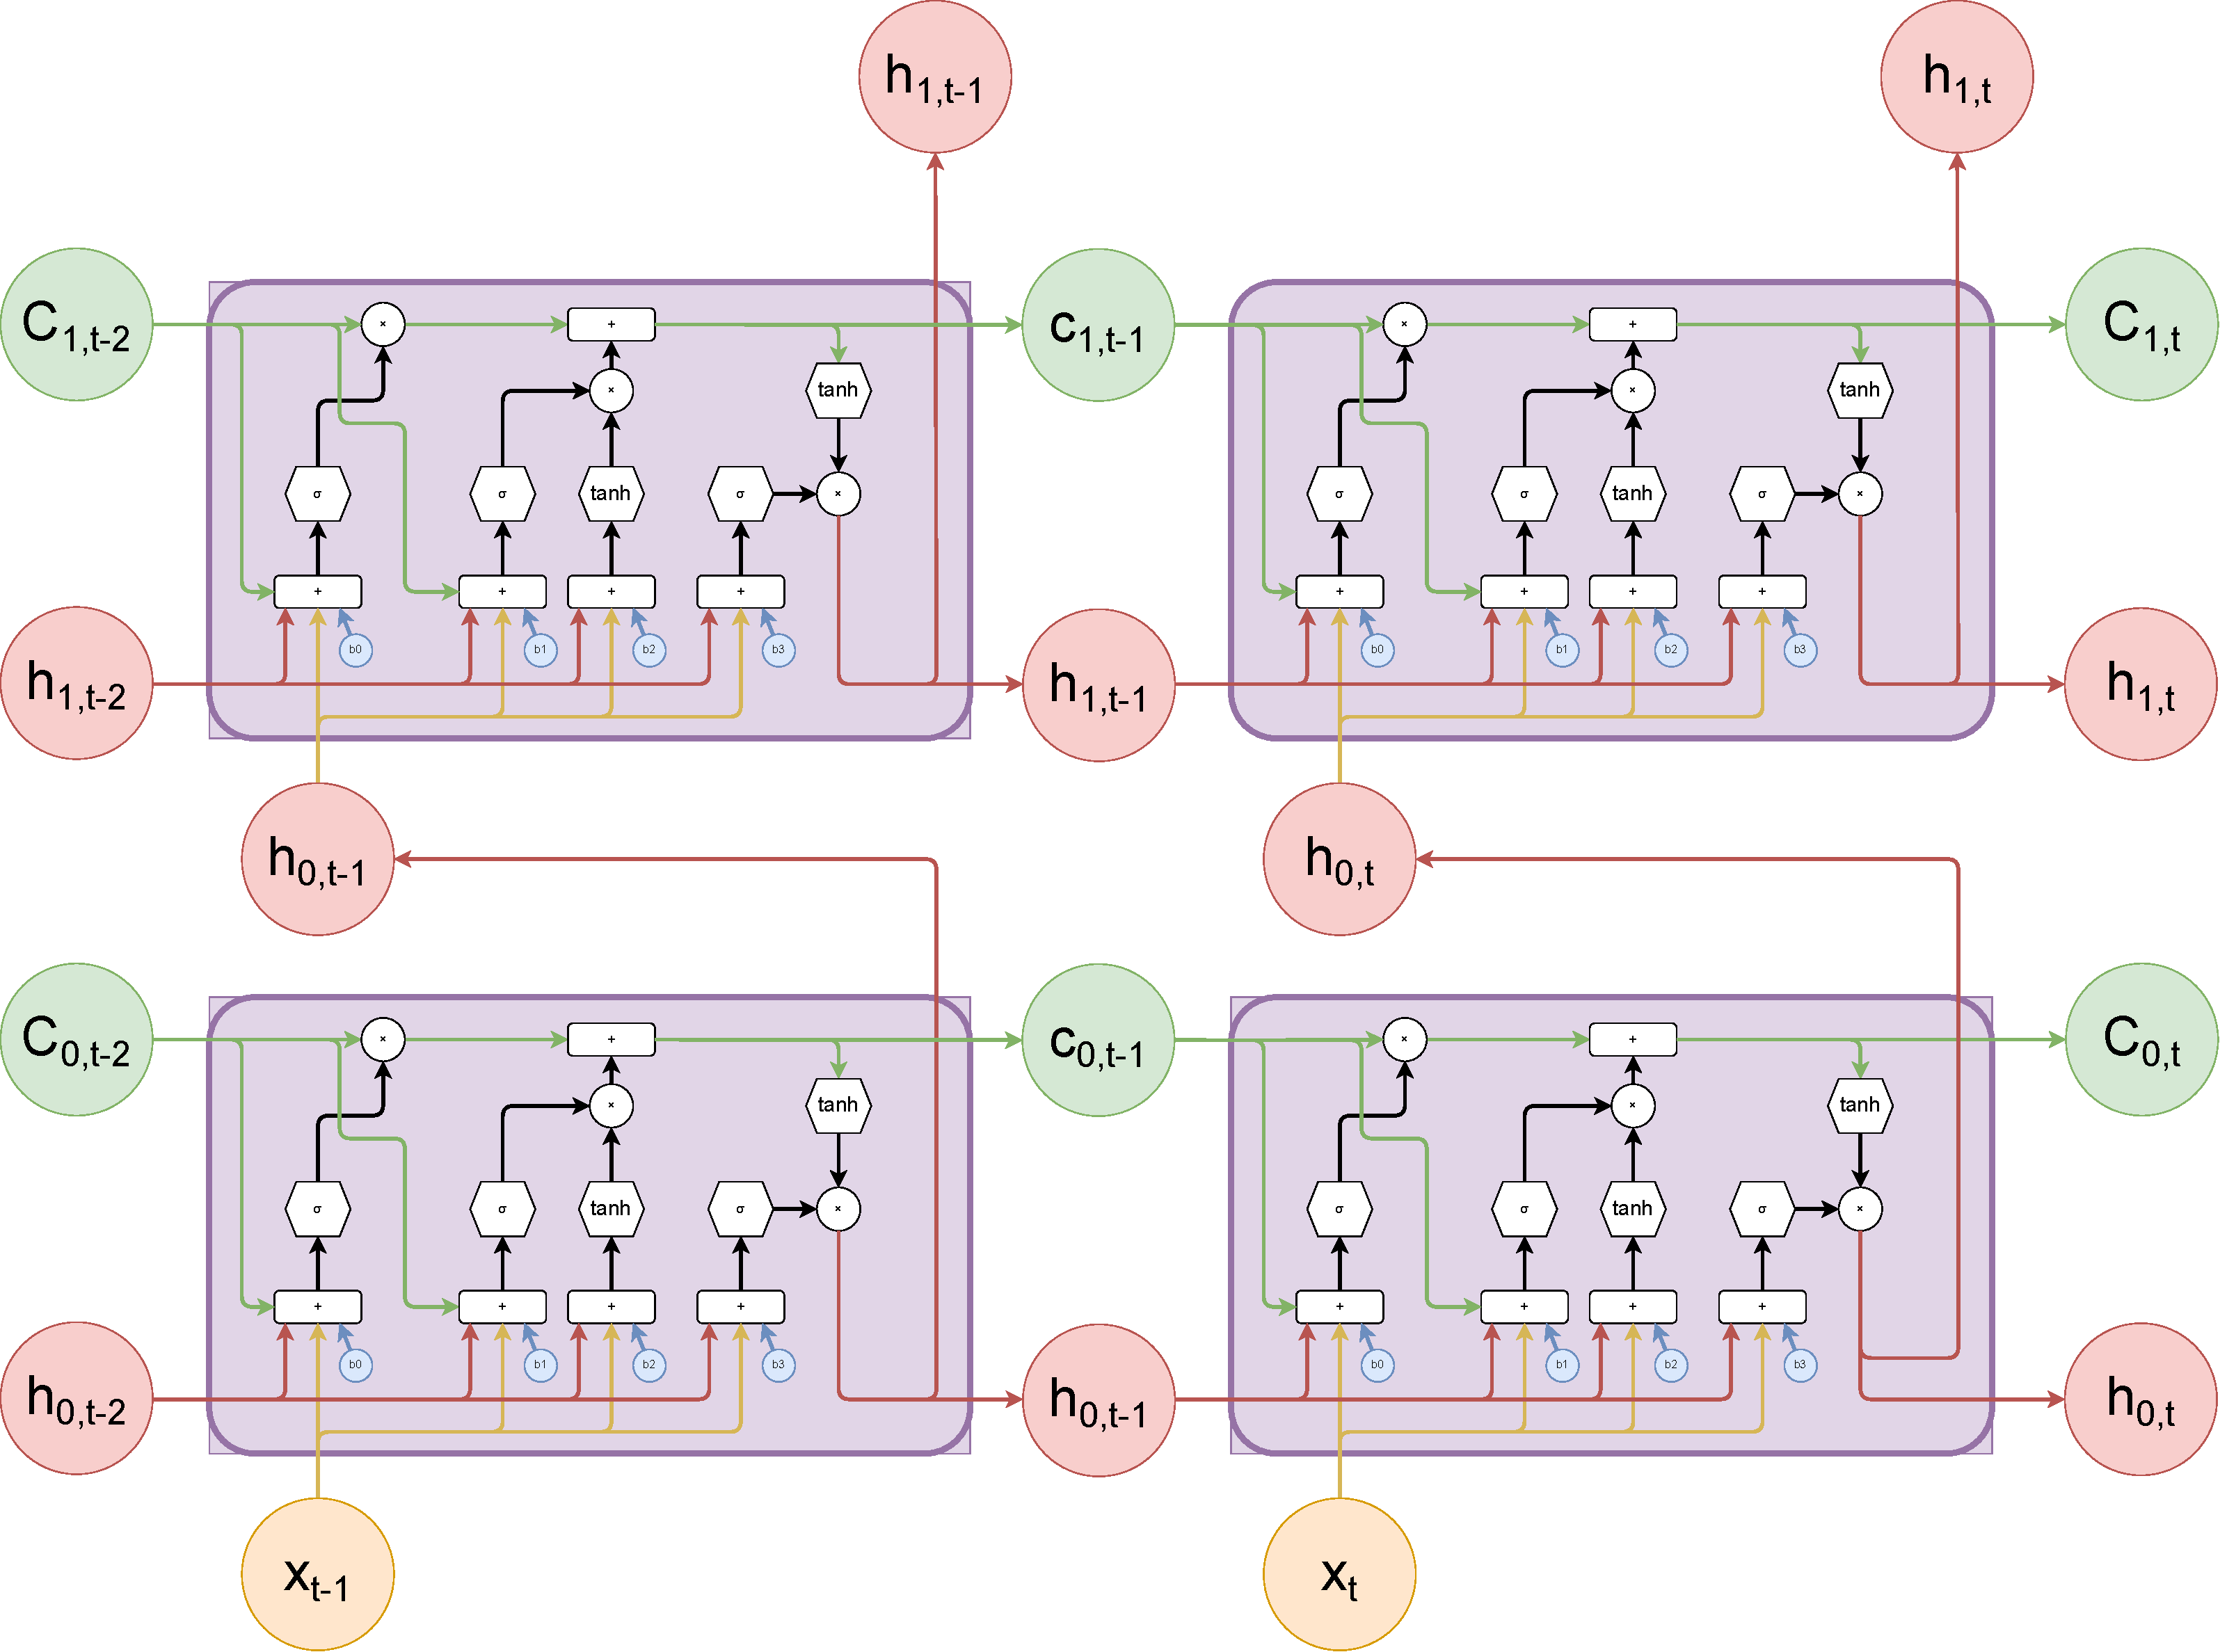
\includegraphics[width=0.70\textwidth]{Figures/LSTM_deep.pdf}
    \caption{Rozvinutá hluboká LSTM síť}
    \label{fig:lstm_deep}
\end{figure}

LSTM sítě vynikají v udržování dlouhodobých závislostí a složitých struktur.
Jelikož mají tři brány, je síť schopná přesně rozhodnout, které informace chce
dlouhodobě uchovávat, které naopak mají větší vliv na aktuální výstup a které
mají být zapomenuty. Je to ale za cenu většího výpočetního nároku a
složitějšího trénování. Také je pro tyto sítě vhodné mít větší množství
trénovacích dat, jinak může dojít k přetrénování. Využívá se tak zejména pro
predikci dlouhých a komplexních časových sekvencí či zpracování přirozeného
jazyka. Zejména u přirozeného jazyka se LSTM sítě osvědčily jako velmi
efektivní. Potřebujeme totiž, aby si síť pamatovala dlouhé závislosti, zároveň
máme většinou k dispozici obrovské množství vzorků.

Síť LSTM by mohla být vhodná pro klasifikaci pózy zejména pokud bychom
potřebovali analyzovat pohyb v delších časových úsecích. Událost pádu se naopak
obvykle odehrává v krátkém čase, nicméně můžeme otestovat, jakých výsledků bude
tato architektura dosahovat oproti jiným rekurentním sítím, zejména v případě,
kdy bychom modelu nepředávali pouze pózu z $n$ posledních snímků, ale celou
sekvenci detekovanou pro danou osobu.

\section{GRU}

Gated Recurrent Unit (GRU) je novější typ rekurentní neuronové sítě, který
představil v roce 2014 Cho et al. \cite{gru}. Je postavený na principu brán,
podobném jako LSTM, nepotřebuje ale zvlášť stav pro dlouhodobou paměť. Místo
toho kombinuje krátkodobou a dlouhodobou paměť do skrytého stavu $h_t$.

\begin{figure}
    \centering
    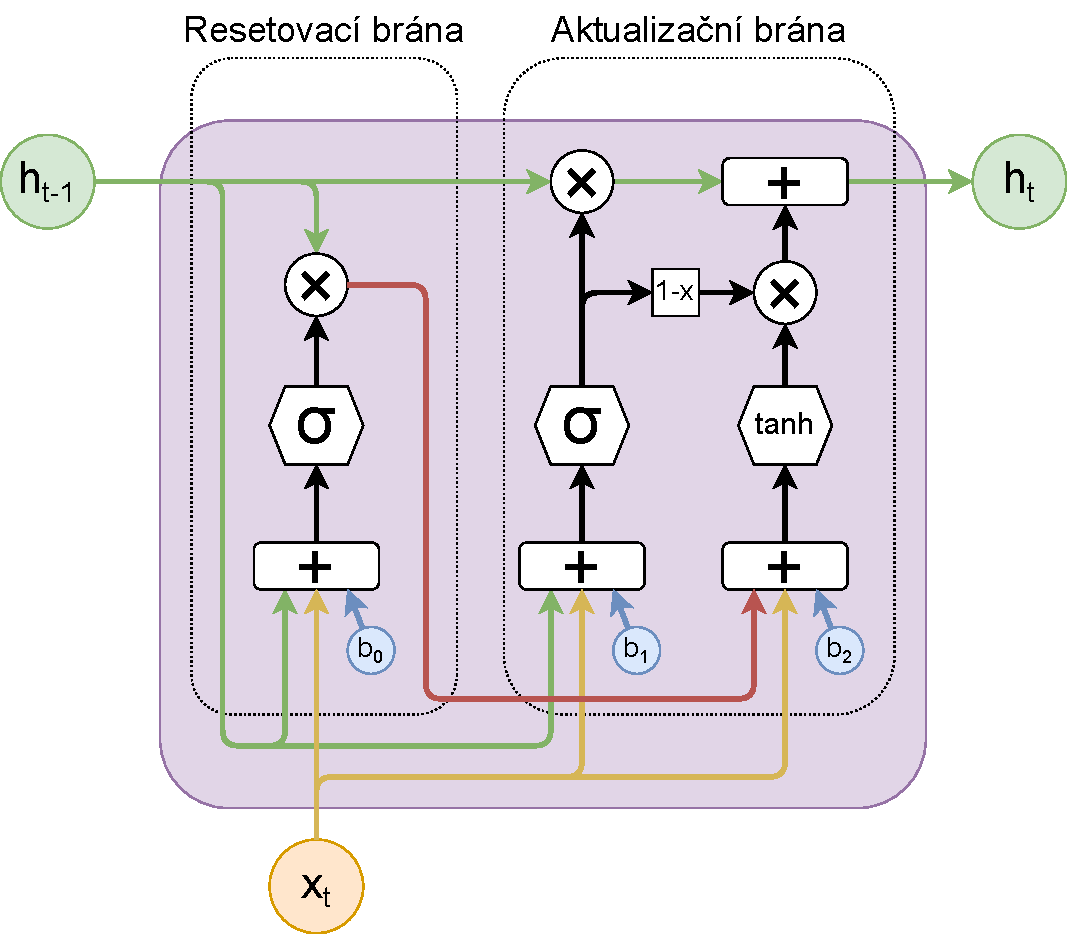
\includegraphics[width=0.6\textwidth]{Figures/GRU_unit.pdf}
    \caption{Jednotka GRU}
    \label{fig:gru_unit}
\end{figure}

GRU obsahuje dvě brány: resetovací bránu (ang. reset gate) a aktualizační bránu
(ang. update gate), viz obrázek \ref{fig:gru_unit}. V resetovací bráně se
určuje, které informace z předchozího skrytého stavu $h_{t-1}$ budou mít vliv
na tvorbu kandidátního skrytého stavu. V aktualizační bráně vzniká nový skrytý
stav $h_t$ kombinací předchozího skrytého stavu a kandidátního skrytého stavu.
Ten je vytvořen pomocí neuronové vrstvy s tangenciální aktivační funkcí, do
které vstupuje výstup resetovací brány a aktuální vstup $x_t$. Pak se na
základě předchozího skrytého stavu $h_{t-1}$ a aktuálního vstupu $x_t$ určí,
které informace v novém skrytém stavu budou převzaty z předchozího skrytého
stavu a které z kandidátního skrytého stavu.

Hlavní výhodou GRU je jednoduchost. Oproti LSTM má méně parametrů a provádí
méně výpočtů. Je tak jednak rychlejší při evaluaci, jednak jednodušší pro
natrénování. Také, u GRU sítí je menší pravděpodobnost přetrénování, což je
výhodné zejména v situacích, kdy máme omezený počet trénovacích dat. GRU sítě
se často využívají v úlohách, kde je důležité rychlé zpracování a efektivita,
např. v mobilních aplikacích a zpracování v reálném čase. Je to ale za cenu
trošku horšího zpracování komplexních a dlouhodobých závislostí. Oproti LSTM
nemá GRU takovou kontrolu nad tím, které informace dlouhodobě uchovávat a má
sklon k rychlejšímu zapomínání. Proto se až tak nehodí pro složitější úlohy a
situace, kdy je nutné si pamatovat velmi dlouhé časové závislosti. Nicméně jsou
dneska první volbou pro mnoho úloh, po LSTM sítích se pak sahá, až když si GRU
sítě s danou úlohou neporadí.

\endinput
% \part{Detekce osob a jejich pozice}
\chapter{Analýza problematiky detekce pádu}
\label{chap:Goal}

V této kapitole stanovíme, co je přesně naším cílem, a zamyslíme se, jak k
našemu problému přistoupit.

Naším úkolem bude v reálném čase z videostreamu detekovat pád osoby. Pád osoby
definujeme jako náhle, neúmyslné klesnutí těla z výškové pozice (např. stání,
chůze nebo sezení) na zem nebo jinou nižší úroveň, přičemž tato osoba nemá
kontrolu nad tímto pohybem. Samozřejmě nejsme vždy schopni úplně dobře
rozeznat, zda se nejedná o úmyslné klesnutí, např. prudké lehnutí.

Dle některých definic (zejména ve zdravotnictví) se o pád nejedná, pokud jde o
důsledek závažné vnitřní příhody (např. mrtvice). V našem případě toto
nerozlišujeme, naopak chceme detekovat jak pády v důsledku ztráty rovnováhy či
vlivem vnějších faktorů (např. zakopnutí, převrácení těžkým předmětem), tak
pády v důsledku akutních události vlivem zdravotních problémů, jako jsou např.
mrtvice, záchvaty, mdloby či jiné důvody ztráty vědomí.

\section{Návrh řešení}

Cílem této práce je navrhnout algoritmus, který bude detekovat, zda je ve
vstupní sekvenci snímku některá osoba, jejíž pozice je klasifikována jako pád.
Hlavním cílem výsledného programu bude alarmovat příslušného pracovníka, pokud
osoba upadne.

Alarmovat budeme až, pokud osoba zůstane v ležící pozici. To nám dá možnost
odfiltrovat falešné alarmy v případě sehnutí či pokud bude osoba špatně
viditelná a algoritmus tak na okamžik špatně vyhodnotí její pohyb. Tímto
postprocesingem se ale teď nebudeme zabývat, spíše se zaměříme na samotnou
klasifikaci pozice.

Stejně jako u detekce objektů, viz \ref{sec:obj_det}, bychom mohli i pro
detekci pádu vytvořit vhodnou konvoluční síť, která by přímo z obrázku
definovala, zda se jedná o pád nebo ne. U detekce se už dnes sice s ohledem na
pokrok hardwaru tento přístup používá, nicméně se jedná o velmi náročný úkol,
který vyžaduje rozsáhlou optimalizaci, pokročilou architekturu a velké množství
trénovacích dat. Nicméně, pokud by se podařilo takovouto síť natrénovat, mohla
by lépe detekovat některé situace např. podle výrazu tváře.

V našem případě tedy budeme v prvním kroku pomocí vhodné předtrénované
neuronové sítě detekovat pozici osoby ve formě klíčových bodů, tuto část
nazvěme \textit{detekční algoritmus}. Na základě těchto bodů pak další
neuronová síť vyhodnotí, zda se jedná o pád, tuto část nazvěme
\textit{klasifikační algoritmus}. To úlohu velice zjednoduší, jelikož místo
analyzování tisíců pixelů, budeme analyzovat pár desítek klíčových bodů. Další
výhodou je, že u takového postupu jsme schopní použít techniky, kdy sledujeme
změny pózy v čase, což by bylo mnohem složitější s jednofázovou konvoluční
síti.

Detekční algoritmus dostane na vstup celý snímek a může detekovat několik osob.
Klasifikační algoritmus ale bude zpracovávat každou osobu, resp. její pózu,
zvlášť.

Další alternativou by mohlo být pouze detekovat osoby jako objekty, a na
základě jejich bounding boxů určit, zda se jedná o pád. Tento postup by byl
jednodušší na dvou úrovních. Jednak je detekce objektů méně náročná úloha než
detekce pózy, jednak bychom ve druhé fázi analyzovali pouze několik parametrů
bounding boxu (rozměry a velikost) oproti pár desítkám klíčových bodů. Nicméně,
pokud se nad tím zamyslíme, ne vždy vypovídají parametry bounding boxů o pozici
člověka. Tento postup by tak pravděpodobně vedl k mnohem méně přesnému
výsledku, než analýza klíčových bodů, kdy může síť analyzovat takové vzorce
jako je např. délka končetin v pohledu či úhel mezi nimi.

Nyní se podíváme, jak budeme pracovat s daty, zejména při trénování, v další
kapitole pak bude rozebraná problematika detekce pózy a bude zvolen algoritmus
pro detekci klíčových bodů. Dále se pak budeme zabývat vývojem modelu
detekujícího pád na základě těchto klíčových bodů.

\section{Trénovací datasety}
\label{sec:TrainingData}

Pro trénování našeho modelu jsme použili necelých 150 krátkých (1 až 15 sekund)
videí ze dvou zdrojů. Prvním je dataset CAUCAFall vytvořený právě pro práci s
pády osob \cite{caucafall}. Tento dataset obsahuje 100 nahrávek simulovaných
pádu v různých světelných podmínkách, s různými osobami. Zahrnují širokou škálu
scénářů, jednak pro různé druhy pádů (v různých směrech či z židle), jednak pro
situace podobné pádu, jako je kleknutí či, sehnutí se, jednak běžné činnosti
jako chůze či sednutí. Poměr videí s úpadkem a bez je 50/50.

Dalším zdrojem pro trénovací data je YouTube video tvůrce Kevina Parryho
\textit{50 Ways to Fall}. Ve videu autor pády v různých scénářích, jako je
zakopnutí, omdlení či poražení elektrickým proudem. Vzhledem k zabavné povaze
videa jsme některé scénáře vypustili, nakonec jsme použili 45 videí. Zde
prakticky všechny videa obsahují pád, v některých se ale postava vrátí do
normálního stavu (např. kotrmelec).

\begin{figure}[]
    \centering
    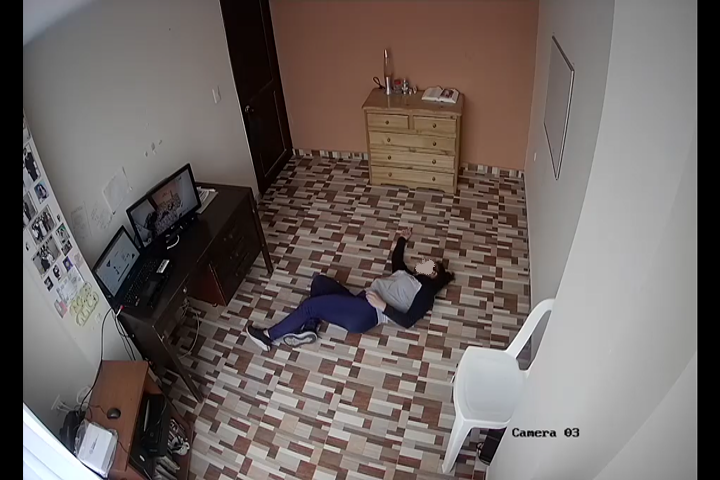
\includegraphics[width=0.45\textwidth]{Figures/datasets_examples/cauca1.png}
    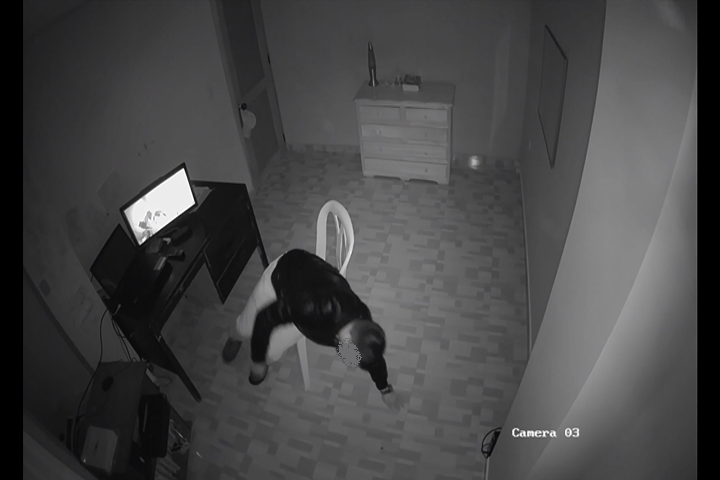
\includegraphics[width=0.45\textwidth]{Figures/datasets_examples/cauca2.png}
    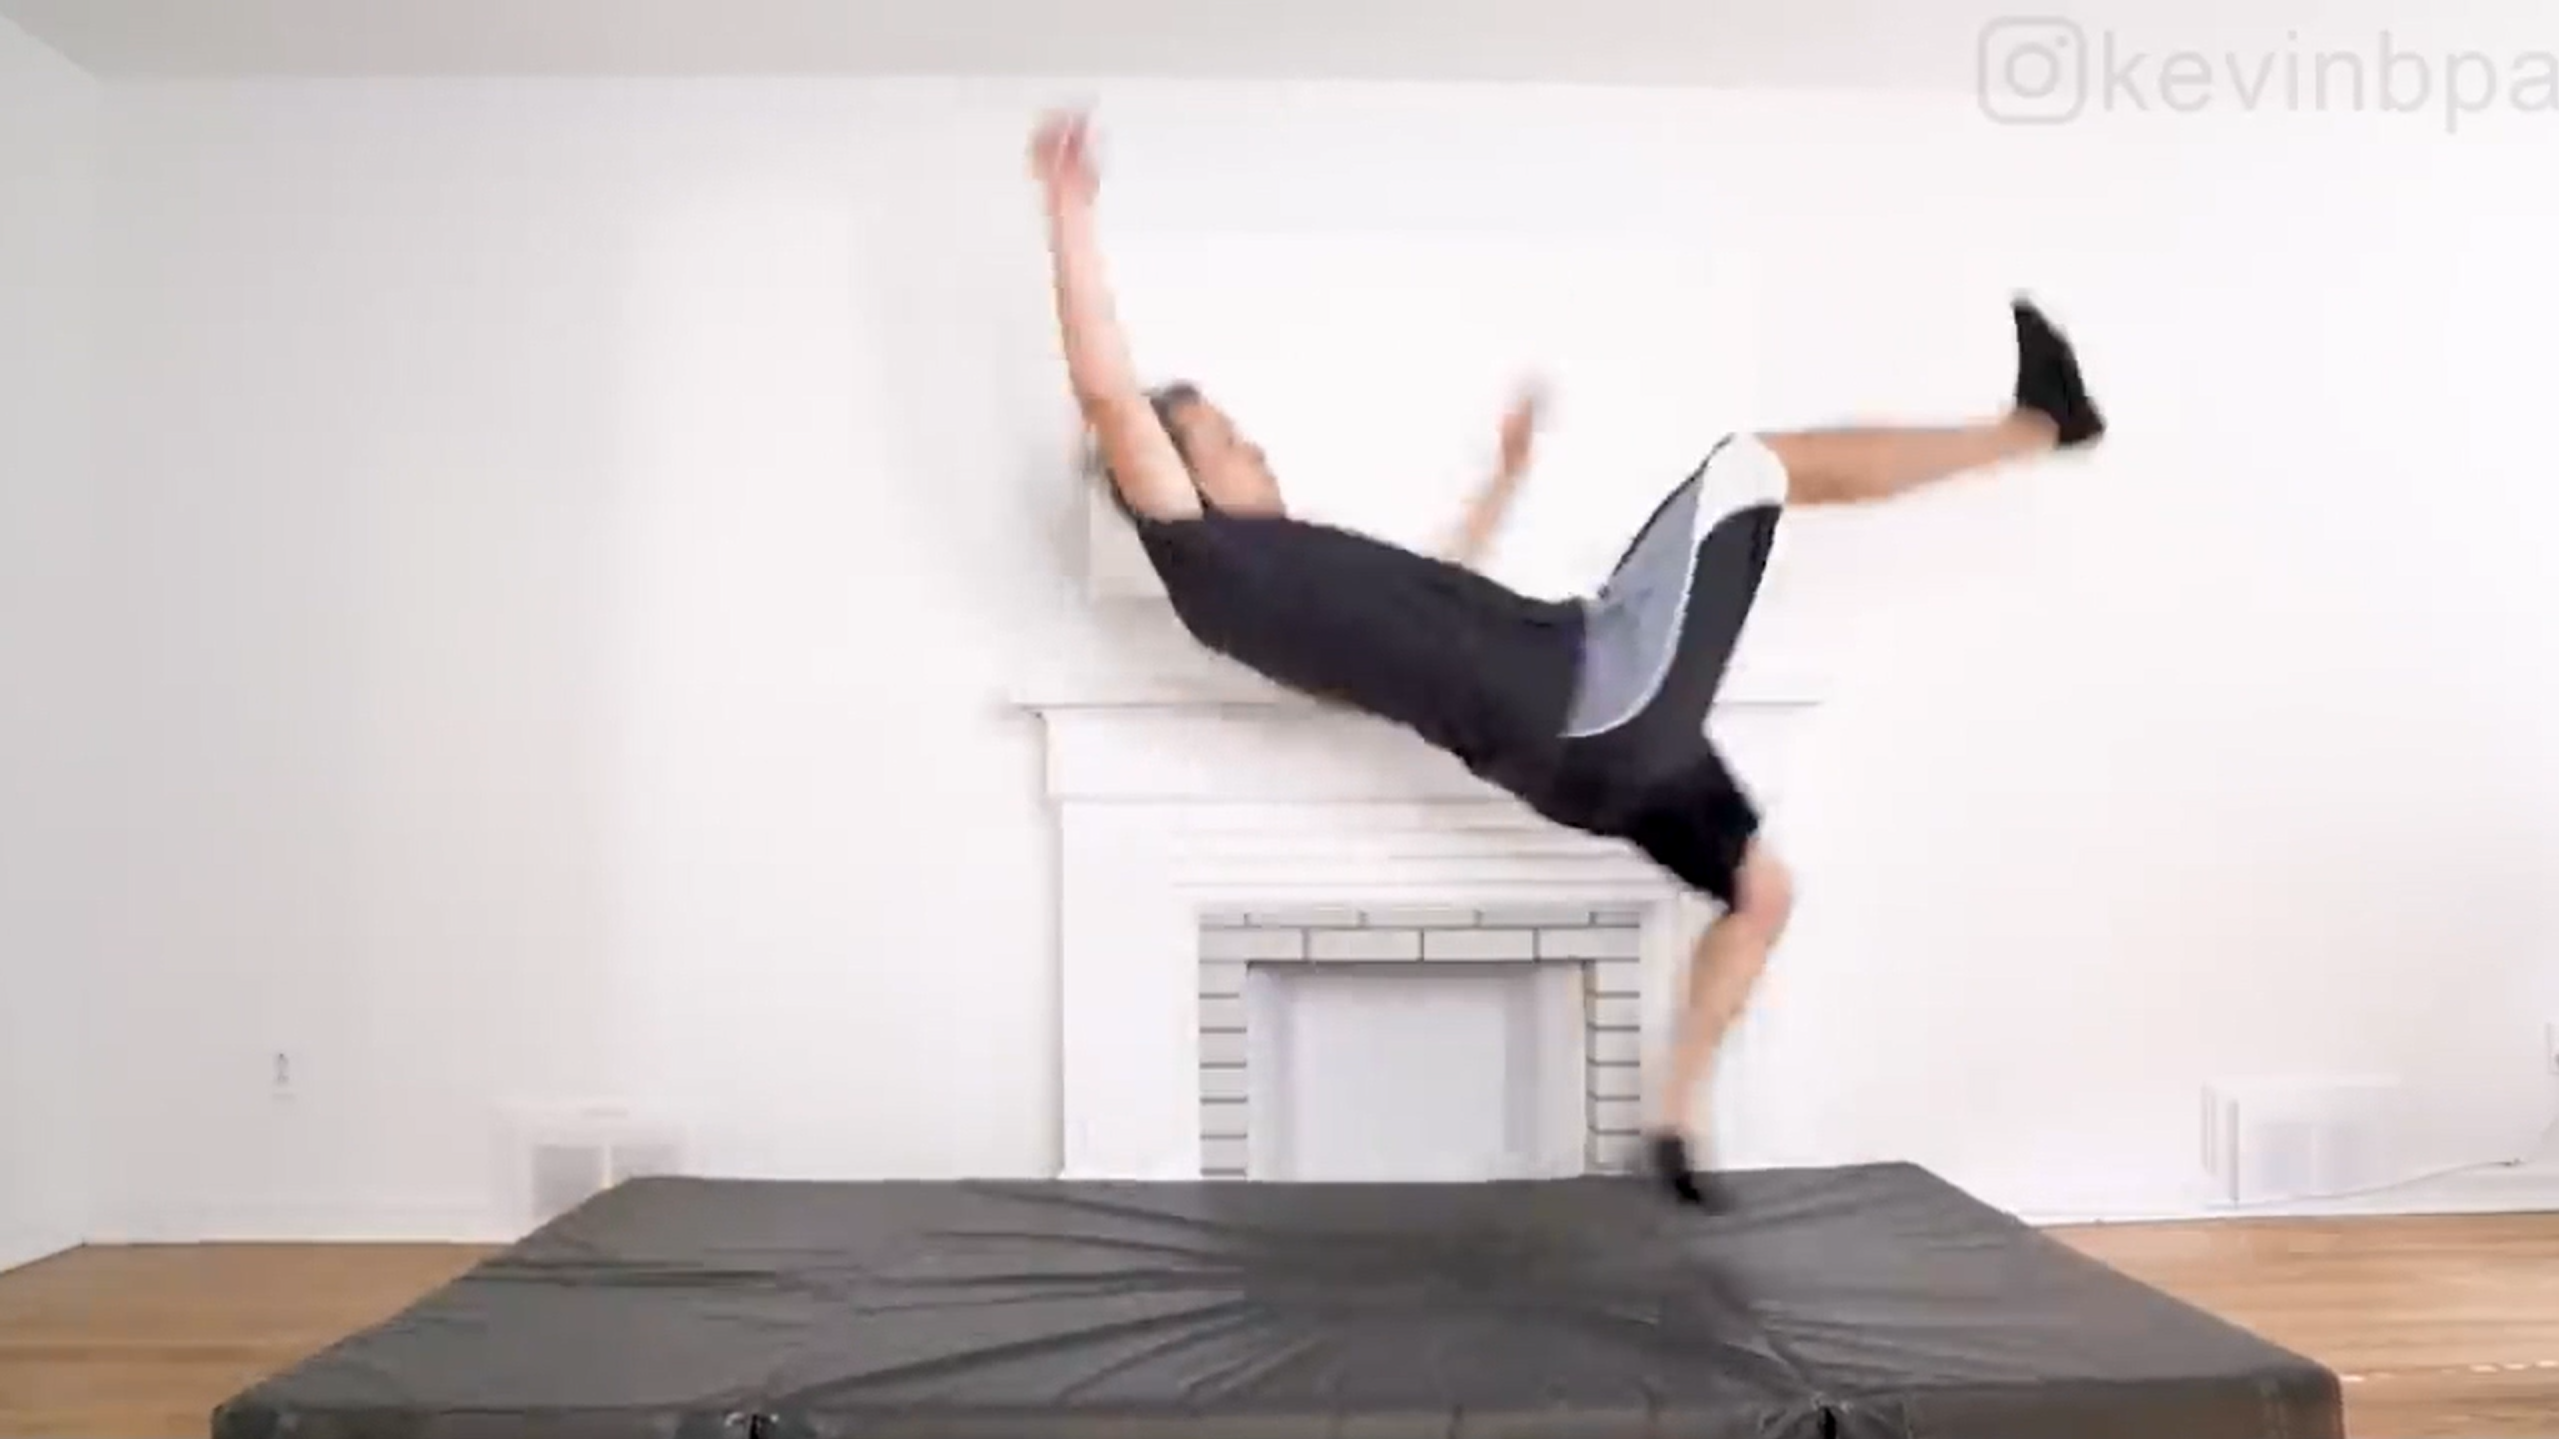
\includegraphics[width=0.45\textwidth]{Figures/datasets_examples/fifty1.png}
    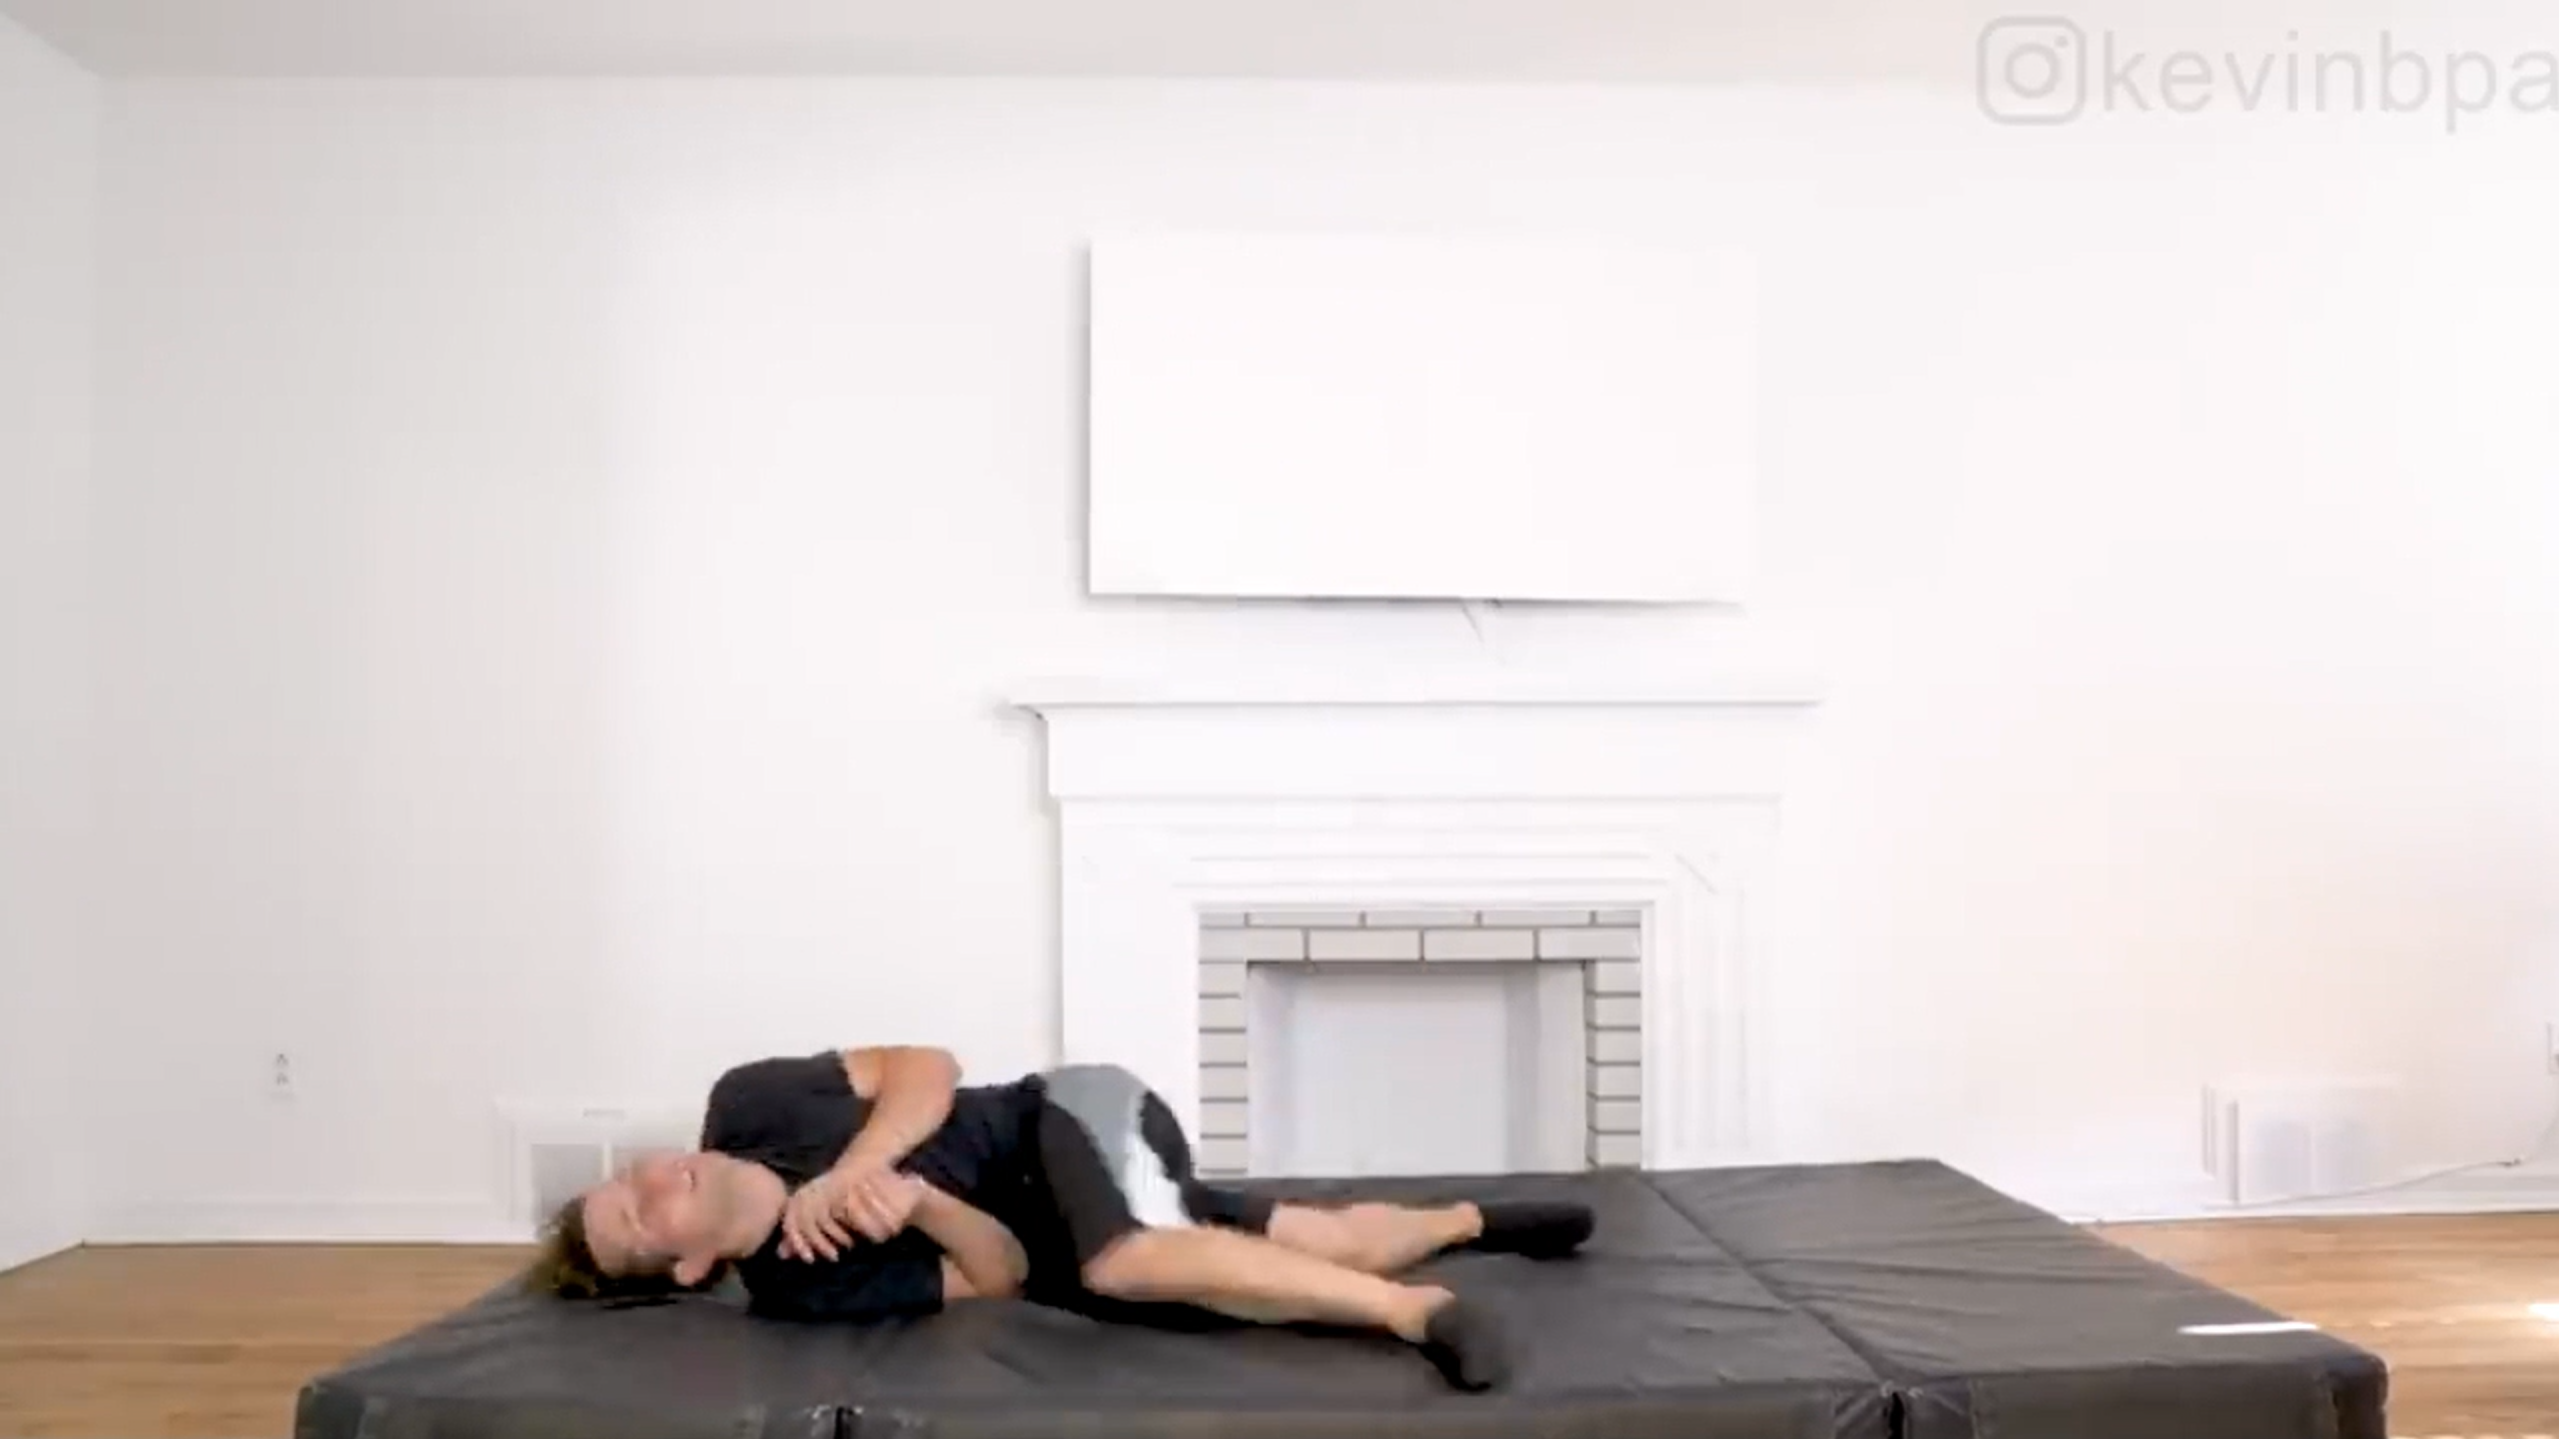
\includegraphics[width=0.45\textwidth]{Figures/datasets_examples/fifty2.png}
    \caption{Příkladové snímky z datasetů CAUCAFall (nahoře) a 50 Ways to Fall (dole).}
    \label{fig:datasets_examples}
\end{figure}

V obou případech se jedná o videa vždy jedné osoby. To proto, že použijeme
detekční algoritmus již natrénovaný na videích s více osobami, a náš
klasifikační algoritmus bude zpracovávat každou osobu zvlášť. Práce s více
osobami tak bude úlohou výsledného detektoru, nikoliv trénované klasifikační
sítě.

Oba datasety jsme rozdělili do tří sad: trénovací, validační a testovací.
Rozděleny byly v tomto poměru: trénovací sada 70\%, validační sada 15\% a
testovací sada 15\%. Trénovací a validační sada budou použity v procesu
trénování – trénovací pro výpočet ztráty a úpravu vah, validační pro průběžné
ověřování výkonu, a testovací sada bude na konci použitá pro otestování jednak
klasifikačního algoritmu, jednak celkového řešení.

\section{Třídy a jejich anotace}
Pro videa byly vytvořeny anotace aktuální třídy pózy. Tato anotace není pro
každý snímek, ale pouze při změně definuje časovou značku a následující třídu.

V anotacích jsme použili 3 třídy, ty odpovídají třem různým třídám pózy, které
nás mohou zajímat – \textit{normální}, kdy osoba např. chodí, sedí nebo stojí,
\textit{padá} – přechodný stav padání, definován od započatí pohybu směrem
dolů, a \textit{upadl} – definován od momentu, kdy se dotkl země trupem nebo
všemi končetinami.

%todo
Pro náš model obecně potřebujeme jenom dvě třídy – \textit{normální} a
\textit{upadl}. Skript tvořící trénovací data proto považuje třídu
\textit{padá} za třídu \textit{normální}. Nicméně by se mohlo do budoucna pro pokročilejší
optimalizaci zkusit experimentovat i se třídou \textit{padá}, která by mohla
síti pomoct hlouběji pochopit problematiku a přesněji rozeznat některé situace,
zejména pak v případě využití rekurentních neuronových sítí.

\section{Příprava trénovacích dat pro klasifikační algoritmus}

Dále byl vytvořen skript, který prošel každé video z trénovacích datasetů a
vytvořil trénovací data pro naši klasifikační síť. Ty obsahují pro každý snímek
detekované klíčové body (jako vstup) a aktuální třídu (jako požadovaný výstup).
Pro detekci klíčových bodů byl použit vybraný model pro detekci pózy. Výběr
modelu je popsán v následující kapitole. Na použitém modelu by teoreticky
nemuselo záležet (pokud detekuje stejné typy klíčových bodů), je ale lepší
použít ve výsledném programu stejný model jako pro trénovací data. Modely se
totiž můžou v některých situacích chovat trochu jinak (např. okluze) a náš
model by tak dostával v praxi jiná data, než pro jaké byl natrénován.

Jelikož pro rekurentní neuronové sítě potřebujeme sekvenci snímků, musí být
trénovací data ještě zpracována. To ale bude již součastí samotného trénovacího
skriptu, jelikož se konečná podoba dat může lišit hlavně délkou sekvencí, dále
ale také dodatečným rozšířením o sekvence vynechávající určité množství snímků,
což simuluje menší snímkovou frekvenci (FPS).

\endinput
\chapter{Výběr algoritmu pro detekci klíčových bodů}
\label{chap:Pose}

Jelikož je dnes dostupných mnoho různých algoritmů či natrénovaných modelů pro
detekci pózy osob v obrázku či videu, nemá smysl pro naše řešení implementovat
takovýto algoritmus od nuly. Možné by to samozřejmě bylo, i vzhledem k
dostupnosti otevřených trénovacích dat (např. dataset COCO \cite{coco}),
nicméně bychom pravděpodobně nedosáhli kvalitních výsledků, jako řešení, která
jsou výsledkem mnoholetých výzkumů. Hlavně pak bychom těžko dosáhli výkonů
těchto řešení, a ten je pro nás stěžejní, jelikož potřebujeme video zpracovávat
v reálném čase.

V následující kapitole budou popsány obecné principy detekce osob a jejich pózy
v obraze. Následně budou popsány některé populární algoritmy pro detekci pózy
se zaměřením na jejich specifika. Několik z nich pak bude otestováno, výsledky
budou porovnány, a na jejich základě bude zvolen algoritmus použitý v konečném
řešení detekce pádu.

\section{Detekce pózy}

\begin{figure}[]
    \centering
    \begin{minipage}{0.48\textwidth}
        \centering
        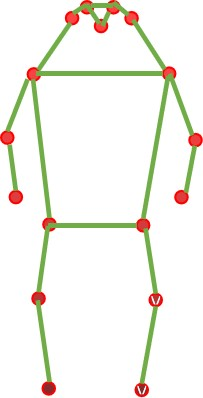
\includegraphics[width=0.5\textwidth]{Figures/keypoints.png}
    \end{minipage}
    \hfill
    \begin{minipage}{0.48\textwidth}
        \centering
        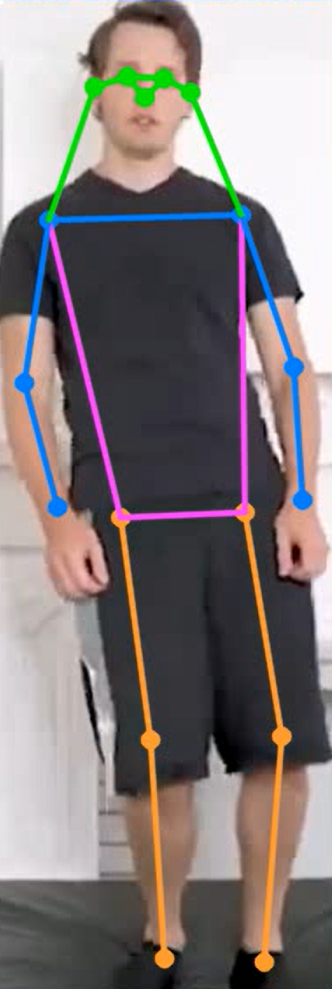
\includegraphics[width=0.35\textwidth]{Figures/pose1.png}
    \end{minipage}
    \caption{(Vlevo) Topologie klíčových bodů použitá např. v COCO-pose \cite{2dhpe} (Vpravo) Příklad detekce pózy pomocí YOLO.}
    \label{fig:keypoints}
\end{figure}

Úloha detekce pózy spočívá v nalezení klíčových bodů postavy v obraze. Může se
jednat také o zvíře, v našem případě se ale budeme zabývat pouze klíčovými body
lidské postavy. Klíčové body představují důležité body lidského těla, znalost
jejich lokalizace nám umožňuje analyzovat pózu dané osoby, popřípadě sledovat
její pohyb. K základním klíčovým bodům patří hlava, ramena, lokty, zápěstí,
kyčle, kolena a kotníky, viz obrázek \ref{fig:keypoints}. Některé algoritmy dokážou
rozeznat i orientaci dlaně či stopy, nebo rozpoznat klíčové body na hlavě, jako
jsou ústa, nos, oči a uši \cite{blazepose}.

Klíčové body jsou většinou reprezentovány jako dvojice souřadnic $(x, y)$
vzhledem k celému obrazu, některé algoritmy poskytují i souřadnice
normalizované vzhledem k bounding boxu osoby. Existují také algoritmy pro 3D
souřadnice, těmito se ale nebudeme zabývat, i když by mohly stanovit zajímavou
alternativu, zejména pokud by pro detekci bylo použito více kamer z různých
pohledů.

V oblasti algoritmů pro detekci pózy existují dva základní přístupy: zdola
nahoru a shora dolů. Přístup zdola nahoru se snaží detekovat všechny klíčové
body v obraze, aniž by rozlišoval jednotlivé osoby, pokud je algoritmus schopen
detekce pózy pro více osob, pak v dalším kroku tyto body spojuje do
jednotlivých postav. Naproti tomu přístup shora dolů nejprve detekuje všechny
osoby v obraze, v jejich rámci pak detekuje klíčové body.

%todo 
\section{Detekce klíčových bodů}

\subsubsection*{Heatmapy}

U obou výše zmíněných přístupů se nejčastěji provádí vyhledání všech klíčových
bodů pomocí tzv. heatmap. Je to 2D mapa pravděpodobnosti, že se v daném bodě
vyskytuje nějaký klíčový bod. Maximální hodnoty v této mapě pak představují
lokalizaci klíčových bodů.

Pro vygenerování heatmap se používá konvoluční neuronová síť. Pro každý klíčový
bod, resp. pro každý typ klíčového bodu k (v případě detekce pózy více osob)
vzniká jedna heatmapa. Jako referenční heatmapy pro trénování se používají
mapy, kde je klíčový bod reprezentován 2D Gaussovým rozložením s vrcholem v
místě daného bodu.

V dalším kroku jsou z heatmap vygenerovány, nejčastěji s pomocí algoritmu
argmax, souřadnice klíčových bodů. V případě vícero osob je pak třeba tyto body
spojit do jednotlivých osob.

\subsubsection*{Regrese}

Využití heatmap je velmi přesné, nicméně z důvodu nutnosti provádění dvou
sekvenčních výpočtů je také trochu pomalé. Také komplikují proces trénování,
jelikož musíme spolu s trénovacími daty dodat modelu i heatmapy. Některé
algoritmy se proto snaží formulovat úlohu jako regresi vedoucí přímo k
souřadnicím klíčových bodů. Tento přístup je ve své podstatě trochu méně
přesný, nicméně je rychlejší.

Vůbec první algoritmus pro detekci pózy využívající hluboké učení, DeepPose
\cite{deeppose}, který byl vytvořen v roce 2014 společností Google, používal
právě regresi. Také algoritmus YOLO používá regresi pro určení souřadnic
klíčových bodů, nicméně detekce je prováděná pro detekované objekty, nikoliv
nad celým vstupním obrazem \cite{yolo-pose}.

% , a je součástí poupraveného modelu pro detekci objektů – v posledních
% vrstvách sítě je kromě regrese definující bounding box a klasifikace určující
% třídu prováděna regrese pro určení klíčových bodů.

\section{Detekce objektů a osob v obraze}
\label{sec:obj_det}

Detekce osob se v podstatě může generalizovat na detekci objektů v obraze.
Detekci objektů v obraze definujeme jako úlohu, kdy ve vstupním obrázku určíme
lokalizaci a třídu všech hledaných objektů. Lokalizace je většinou
reprezentována jako souřadnice obdélníku ohraničujícího daný objekt, tzv.
bounding box.

V kapitole \ref{chap:CNN} jsme si popsali základní architekturu konvolučních
neuronových sítí, ta se ale většinou v praxi používá pro klasifikaci obrázků,
nikoliv pro detekci objektů – algoritmus tedy pouze určí, o jakou třídu objektu
se jedná, a ideálně potřebuje, aby objekt vyplňoval celý vstupní obraz.
Teoreticky by bylo možné detekci formulovat jako regresní problém a natrénovat
takovou síť, která by pomocí několika konvolučních vrstev následovaných
několika plně propojenými vrstvami byla schopna predikovat lokalizaci a třídu
všech objektů v obraze \cite{szegedy}. Problém detekce je ale velice komplexní
a také by vyžadoval velice komplexní síť – více vrstev s mnoha filtry, resp.
neurony. Jak již ale bylo zmiňováno, komplexnost sítě zvyšuje její nároky na
výpočetní výkon a komplikuje nebo úplně znemožňuje její trénování s ohledem na
pravděpodobnost přetrénování.

Snahou tedy bylo najít metody, které poupraví architekturu sítě tak, aby byla
schopna efektivní detekce objektů. Většina těchto metod se nějakým způsobem
snaží rozdělit vstupní obrázek na menší části, ty následně jednak klasifikovat,
a tedy určit, zda se v dané lokalitě vyskytuje objekt, popřípadě pomocí regrese
určit jeho přesnou lokalizaci. Rozdělení může být provedeno přímo na vstupním
obrázku nebo na mapě příznaků v rámci sítě.

Metoda sliding window (klouzavé okno), která aplikuje hrubou sílu a projde
veškeré možné oblasti, je samozřejmě velice neefektivní, a tak se další metody
snaží buď najít pouze oblasti, ve kterých je pravděpodobné, že se nějaký objekt
nachází – dvoufázový přístup, anebo rozdělí obrázek do mřížky – jednofázový
přístup.

Jelikož jsou tyto metody základem pro většinu detektorů klíčových bodů, pojďme
si několik základních popsat.

% \subsection{Sliding window}

% Jednou z prvních takových metod byl tzv. sliding window (klouzavé okno), který
% aplikuje hrubou sílu. Vstupní obrázek se postupně projíždí oknem o fixní
% velikosti. Vznikne tak množina pokrývající každou možnou lokaci objektů. Na
% tyto oblasti se pak aplikuje klasifikační algoritmus. Postup se opakuje pro
% několik velikostí okna, aby se detekovaly objekty různé velikosti.

% Tento postup je ale velice pomalý, jelikož je pro každý obrázek zvolený velký
% počet oblastí, pro které je třeba provést klasifikaci popřípadě regresi. Navíc
% je většina těchto oblastí prázdná, a dochází tak k plýtvání výpočetním výkonem.
% Algoritmus se také potýká s překrývajícími se objekty.

% Další metody se tedy snaží redukovat počet oblastí, na které se aplikuje
% klasifikace, tak, že se vybere pouze oblasti, které pravděpodobně budou
% obsahovat nějaký objekt.

\subsection{Dvoufázový přístup}

\subsubsection*{R-CNN}
Prvním algoritmem, který efektivně zredukoval počet oblastí pro klasifikaci,
byl algoritmus R-CNN (Region-based Convolutional Network) \cite{r-cnn}. Tento
algoritmus nejprve použil některou z dostupných metod (autoři použili selective
search) pro vygenerování navržených oblastí (region proposals), které
pravděpodobně obsahují nějaký objekt. Tyto metody jsou nezávislé na třídě
objektů. Algoritmus tedy vygeneruje zhruba 2000 oblastí, vzniklé obrázky jsou
následně upraveny na velikost požadovanou CNN v další fázi. CNN extrahuje z
dané oblasti mapu příznaků, na její základě plně propojené vrstvy predikují
třídu objektu popřípadě jeho bounding box.

Problémem R-CNN je, že výběr oblasti a jejich následná klasifikace jsou
nezávislé úlohy a jsou nezávisle trénovány. Detekce objektu je také poměrně
pomalá, protože je extrakce příznaků prováděná pro všechny oblasti zvlášť. Tyto
problémy se snaží řešit další upravené verze R-CNN.

\subsubsection*{Fast R-CNN}
První z nich je Fast R-CNN \cite{fast-r-cnn}, která je upravená tak, aby bylo
možné provádět trénování v jednom kroku. Také extrahuje příznaky pro celý
vstupní obraz najednou, pomocí selective search pak identifikuje oblasti zájmu
(ang. region of interest – RoI), které následně použije pro klasifikaci a
regresi. Tato metoda je přesnější a asi desetkrát rychlejší než původní R-CNN.

\subsubsection*{Faster R-CNN}
Další algoritmus, Faster R-CNN \cite{faster-r-cnn}, nahrazuje metodu selective
search vlastní, plně konvoluční sítí RPN (region proposal network).
Zefektivňuje tak proces trénování, výsledná síť je také rychlejší a přesnější
než Fast R-CNN.

\subsection{Jednofázový přístup}

Jednofázový přístup se snaží najít řešení, ve kterém není nutné hledat navržené
oblasti, ale provést klasifikaci a regresi na předem dané množině oblastí,
obvykle určené mřížkou.

\subsubsection*{YOLO}
Prvním takovým algoritmem byl YOLO (také YOLOv1, z ang. you only look once)
\cite{yolo}. Ten, v původní verzi, rozdělí vstupní obraz do pevně dané mřížky
velikosti $S \times S$ a v každém z těchto polí určí $B$ bounding boxů a jejich
třídu. V původní verzi bylo zvoleno $S = 7$ a $B = 2$.

Obraz je nejprve zpracován pomocí konvolučních vrstev, které extrahují mapu
znaků o velikosti $S \times S \times K$, kde $K$ je počet kanálů. Každý pixel
této mapy představuje jedno pole mřížky. Dále je mapa zpracována plně
propojenými vrstvami, které provádějí nad každým polem mřížky klasifikaci a
regresi, viz obrázek \ref{fig:yolo}.

\begin{figure}[]
    \centering
    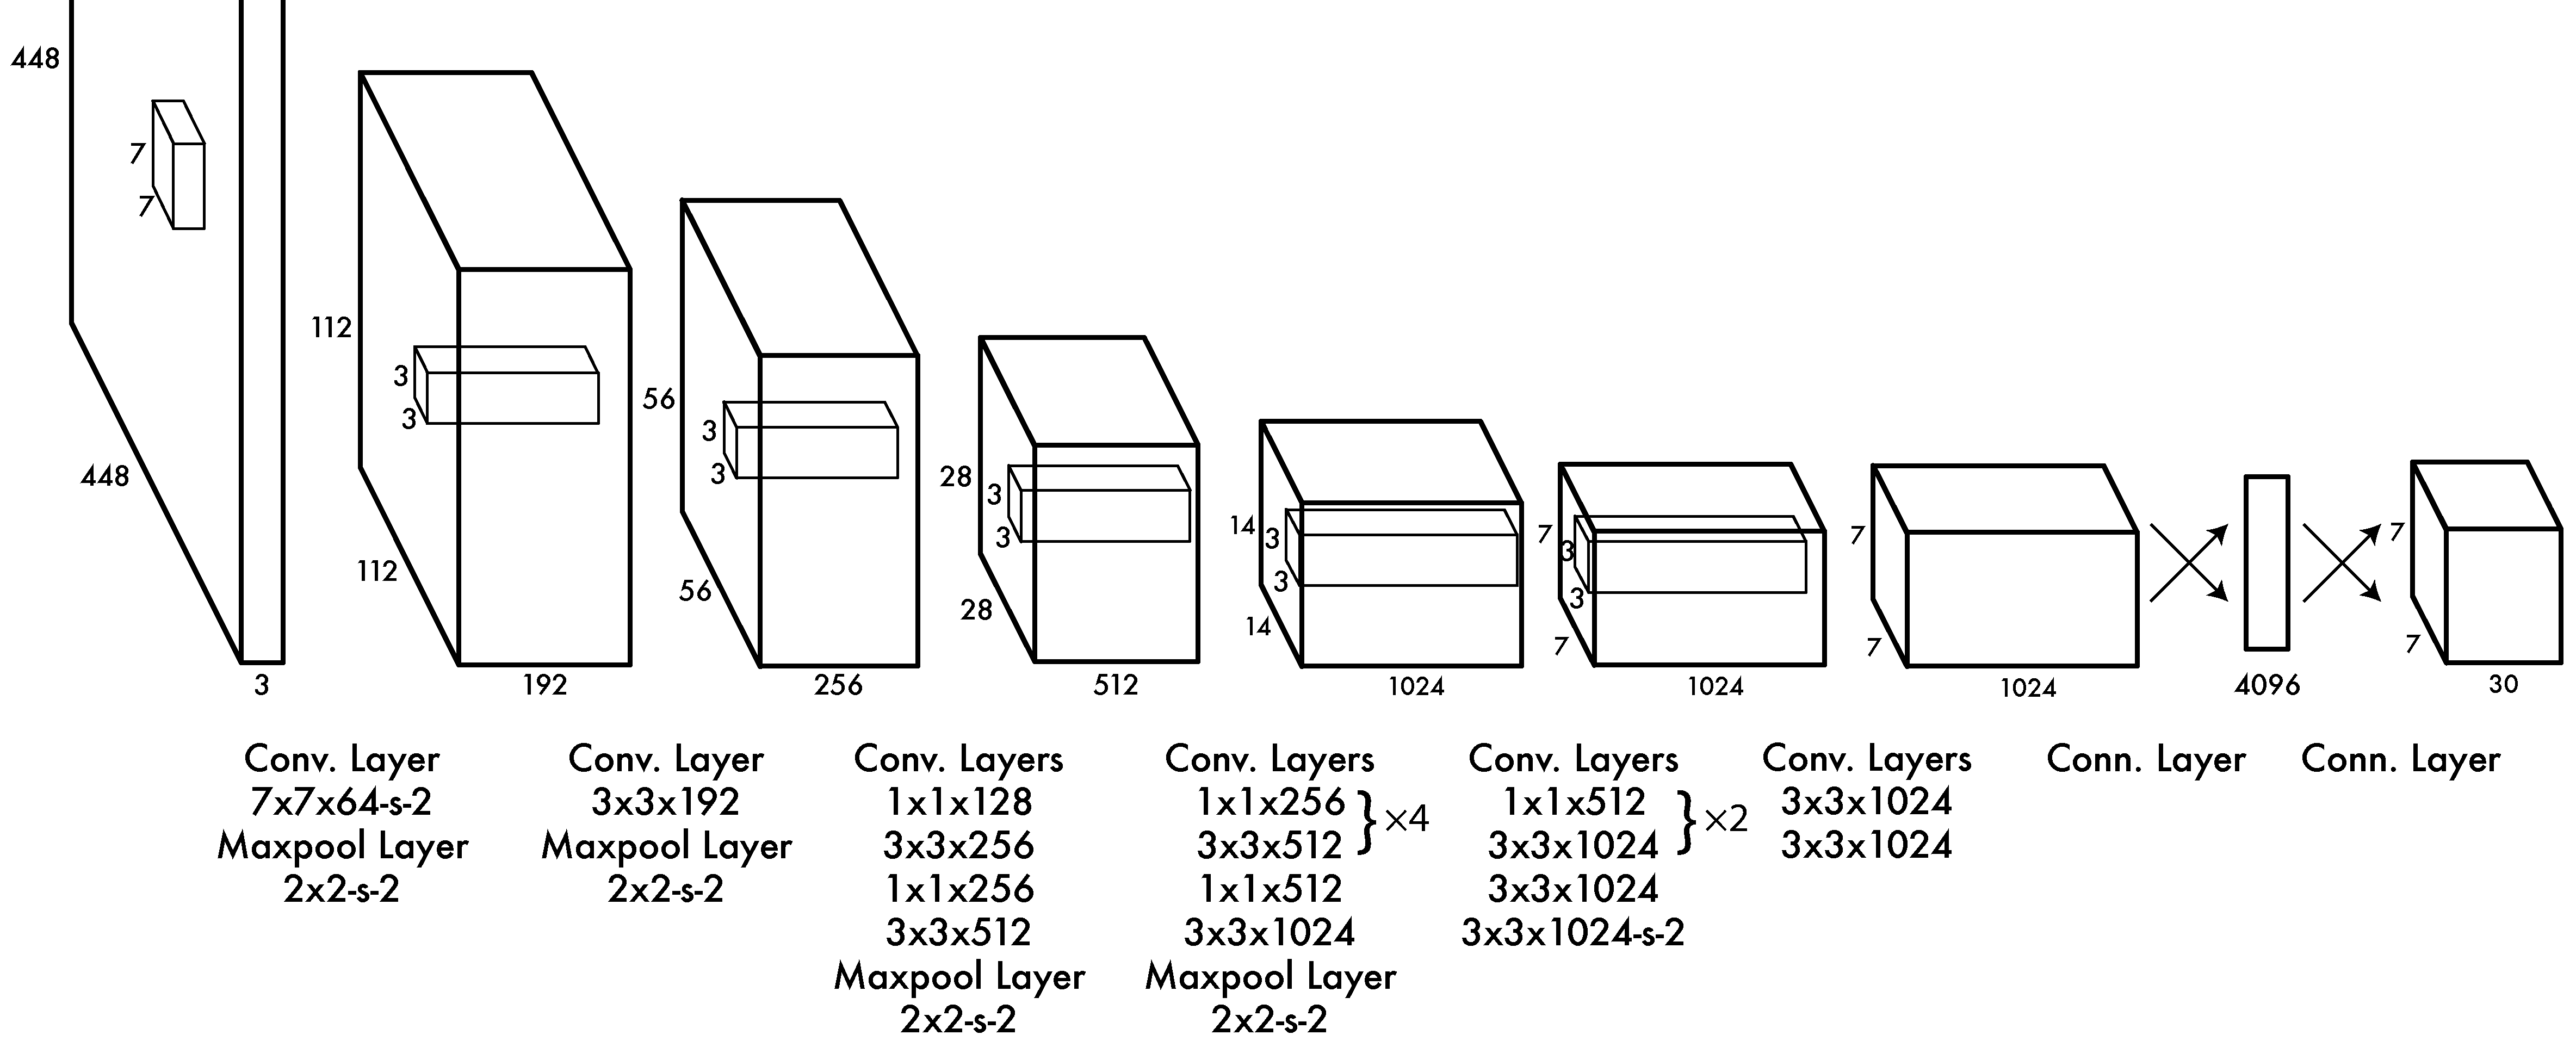
\includegraphics[width=0.8\textwidth]{Figures/yolo}
    \caption{Architektura původní verze YOLO \cite{yolo}}
    \label{fig:yolo}
\end{figure}

Každý bounding box je reprezentován souřadnicemi středu a velikosti (šířka a
výška). Dohromady s informací o jistotě detekce bounding boxu (confidence
score) vrátí model $5$ informací o každém bounding boxu. Pro každé pole mřížky
pak určí společnou informaci o třídě všech objektů v daném poli. Pokud objekt
není detekován, třída indikuje pozadí a souřadnice bounding boxu jsou
ignorovány. Velikost výstupního vektoru je tedy $7 \times 7 \times (2 * 5 +
    C)$, kde $C$ je počet definovaných tříd – v původní verzi pouze 20.

Tento algoritmus, navržený v roce 2015 J. Redmonem et al., byl revolučně
rychlý, zároveň v porovnání s jinými real-time detekčními algoritmy dosahoval i
slušné přesnosti. Nicméně byl velice citlivý na velikost objektu a přesnost
detekce, zejména u menších objektů, byla horší než u dvoufázových algoritmů.

Další verze algoritmu YOLO přinesly postupná vylepšení ve formě optimalizace
trénování a architektury. YOLOv2 \cite{yolo9000} zavedl mj. trénování na
několika měřítkách a byl natrénován s 9000 třídami (proto také nazýván
YOLO9000). YOLOv3 \cite{yolov3} přinesl mj. detekci na několika měřítkách.
Postupně byla také zvětšována mřížka a měnila se použitá architektura CNN sítě
sloužící pro extrakci příznaků pro jednotlivá pole mřížky. Postupně také byly
přidávány další funkce jako je segmentace, detekce pózy či sledování objektů
(ang. tracking).

V 2020 roce firma Ultralytics poprvé implementovala YOLO s využitím populární
knihovny PyTorch (YOLOv5), což umožnilo snadnější využití YOLO v praxi. Firma
Ultralytics také vytvořila framework pro použití různých verzí YOLO (YOLOv3 a
novější). Také pracuje na dalších vylepšeních a optimalizacích. Konkrétně
vytvořila YOLOv5 (2020), YOLOv8 (2023) a YOLOv11 (2024). Tyto verze nicméně
nejsou podloženy odbornými články, někteří je tak považují za neoficiální
verze.

\subsubsection*{SSD}
Dalším populárním algoritmem, který používá jednofázový přístup, je SSD (z ang.
single shot detector) \cite{szegedy:ssd}. Ten rozdělí vstupní obraz do několika
mřížek o různé velikosti. Postup je takový, že nejprve projde obraz konvoluční
sítí, konkrétně sítí VGG16, která extrahuje mapu příznaků. Tu se postupně
dalšími konvolučními vrstvami zmenšuje, výstup každého stádia zmenšení,
reprezentující mřížku dané velikosti, se spolu s původní mapou dále zpracovává
plně propojenou sítí.
\begin{figure}[]
    \centering
    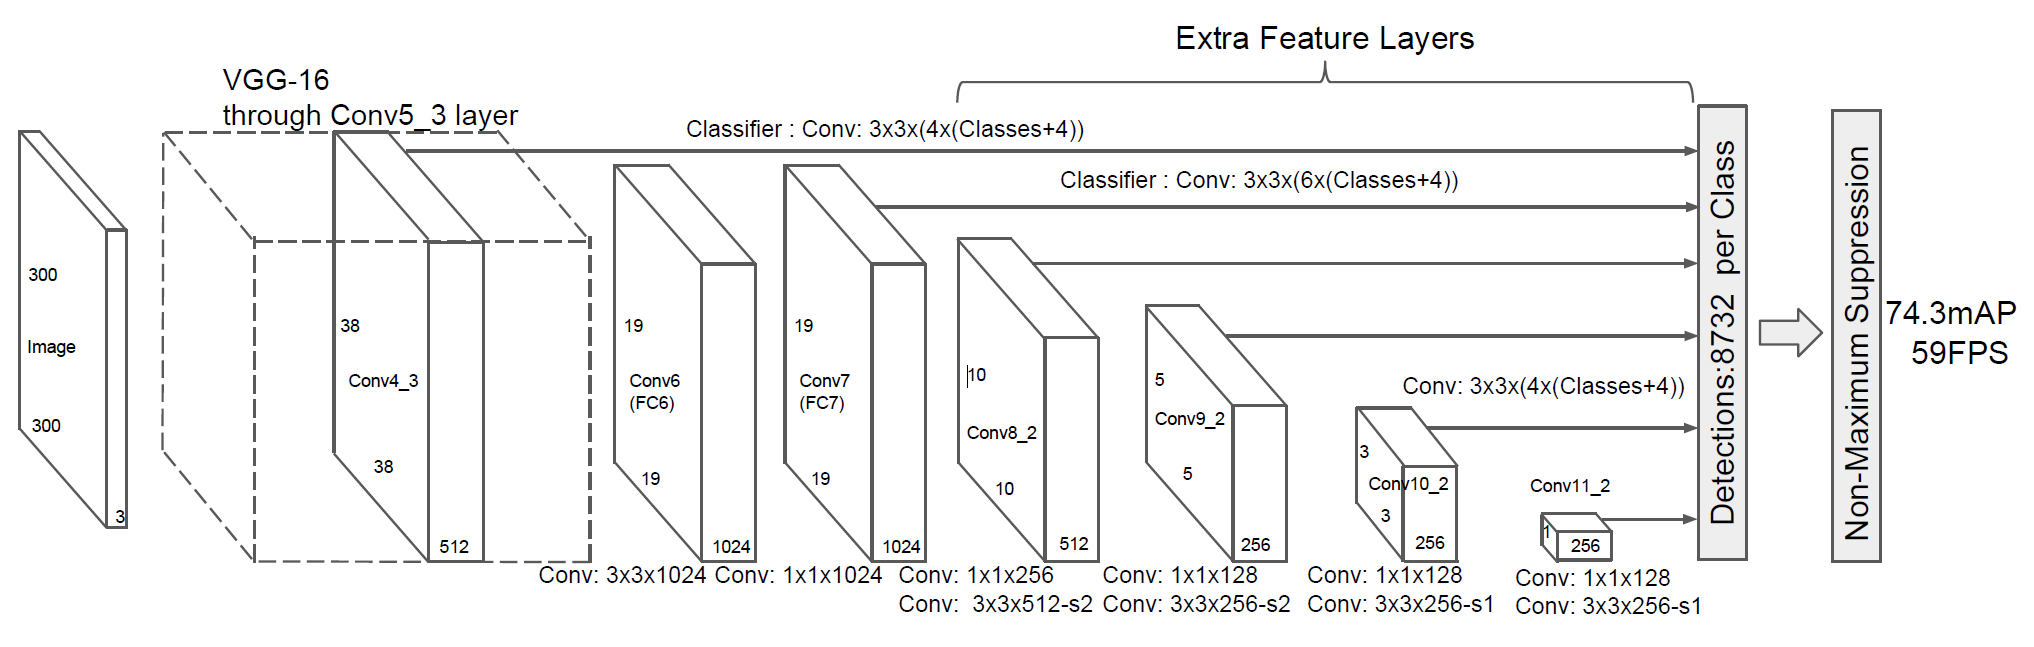
\includegraphics[width=0.8\textwidth]{Figures/ssd.png}
    \caption{Architektura SSD \cite{szegedy:ssd}}
    \label{fig:ssd}
\end{figure}

Výstupní bounding boxy nejsou, jako v případě YOLO, pouze výsledkem regrese,
ale pro každé pole dané mřížky je definováno několik výchozích oblastí (ang.
default box), ze kterých jsou vybrány ty, které obsahují objekt. K ním je
predikována třída objektu a posun i změna velikosti výchozí oblasti,
upřesňující výsledný bounding box.

V době svého vzniku byl SSD rychlejší a přesnější než YOLO, ale novější verze
YOLO jej už předběhly. Nicméně některé principy SSD, jako výchozí oblasti či
použití různých měřítek, byly převzaty do novějších verzí YOLO.

\section{Charakteristiky vybraných implementací pro detekci pózy}

V této sekci bude popsáno několik populárních algoritmů (a jejich implementací)
pro detekci pózy, zejména se zaměřením na jejich rychlost, přesnost a specifika
architektury.

Velká část algoritmů byla zamítnuta a neproběhlo ani jejich testování.
Nejčastějším důvodem zamítnutí některého z algoritmů je, že schází jeho volně
dostupná, aktualizovaná implementace. Tvůrci algoritmů většinou investují čas a
zdroje pro vývoj algoritmu a natrénování modelu (často pro akademické účely),
pak ale neinvestují do jeho údržby. Zejména v prostředí Pythonu, kde se
neustále vyvíjejí nové knihovny a zpětná kompatibilita starších verzí není
zaručena, je pak obtížné použít takovéto řešení ve svém projektu, aniž by bylo
nutné investovat další čas do pochopení zdrojového kódu a jeho úpravy. Jak již
bylo zmíněno na počátku kapitoly, implementace algoritmu od nuly by vyžadovala
velké množství času a zdrojů (zejména výpočetních), hlavně by také byla
potřebná hlubší znalost problematiky. Někdy je možné řešení použít za cenu
kompromisu ve formě použití starších verzí knihoven či Pythonu, může to ale
představovat bezpečnostní rizika. Také některé algoritmy jsou sice volně
dostupné, ale jejich implementace jsou součástí komerčních produktů, např.
OpenPose, jež je mj. součástí produktu Viso Suite od viso.ai
\cite{visoai_openpose}.
\subsection{DeepPose}
DeepPose je historicky první algoritmus pro detekci pózy využívající hluboké
učení. Vyvinuli jej Alexander Toshev a Christian Szegedy ze společnosti Google
v roce 2014 \cite{deeppose}. Algoritmus předpokládá, že se ve vstupním obraze
nachází pouze jedna osoba. Síť se snaží v jednom kroku pomocí regrese jak
detekovat osobu, tak i její klíčové body. Jelikož je těžké takto dosáhnout
velmi přesných výsledků, algoritmus používá další fázi, která pomocí regrese
provádí posun bodů k přesnějším výsledkům. Tato fáze je aplikována opakovaně,
kaskádně se tak zvyšuje přesnost detekce.

Při svém vzniku byl DeepPose revoluční, nicméně v porovnání s dnešními řešeními
je poměrně pomalý a nepřesný. Nicméně položil základ pro využití hlubokého
učení v oblasti detekce pózy.

\subsection{OpenPose}

OpenPose \cite{openpose} je typicky příklad přístupu zdola nahoru. Jeho výhodou
je ale možnost vyhledání více osob v jednom snímku. Tento algoritmus, který
vyvinuli v roce 2019 Zhe Cao et al., nejprve pomocí CNN vytvoří heatmapu pro
každý typ klíčového bodu. Pro spojení bodů do jednotlivých osob využije pole
propojení klíčových bodů (ang. part affinity field – PAF). PAF je mapa
vytvořená pro každou končetinu (myšleno obecně spojení dvou klíčových bodů),
která v oblasti dané končetiny obsahuje hodnoty určující směr z jednoho bodu do
druhého. Pokud pak dáme do hromady informace z heatmap a z PAF, jsme schopni
poměrně jednoznačně zkompletovat jednotlivé klíčové body do celých postav.
Stejně jako heatmapy, jsou i PAF součástí trénovacích dat.

\subsection{OpenPifPaf}

Algoritmus OpenPifPaf \cite{openpifpaf}, vyvinutý v roce 2021 Svenem Kreissem
et al., je v podstatě vylepšenou verzí OpenPose. Jeho název je odvozen od dvou
stavebních kamenů: PIF (Part Intensity Field) – pole intenzity klíčových bodů,
a PAF (Part Affinity Field) – pole propojení klíčových bodů. PIF je rozšířením
heatmap, kdy kromě intenzity pravděpodobnosti klíčového bodu obsahuje i jeho
posun, zaručující přesnější lokalizaci bodu, a odhadovanou velikost dané části
těla. PAF v OpenPifPaf je také podobný tomu v OpenPose, navíc ale indikuje
kromě směru i velikost dané končetiny, což umožňuje lepší prostorové zachycení
pózy.

Dalším rozšířením oproti OpenPose je možnost sledování osob ve videu. Mapa
příznaků, která je výsledkem vstupní CNN, je udržována v mezipaměti, do další
části sítě pak vždy vstupují mapy pro aktuální a předchozí snímek. Výstupem pak
kromě klíčových bodů v každém snímku a jejich propojení tvořící kostru, jsou i
propojení mezi klíčovými body z jednotlivých snímků, viz
\ref{fig:pipaf-tracking}. Algoritmus si pak udržuje ID sledovaných osob, pokud
k dříve nalezené osobě je nalezena nová pozice, je jí přiřazeno stejné ID.
Pokud je nalezena nová osoba, je jí přiřazeno nové ID.

\begin{figure}[]
    \centering
    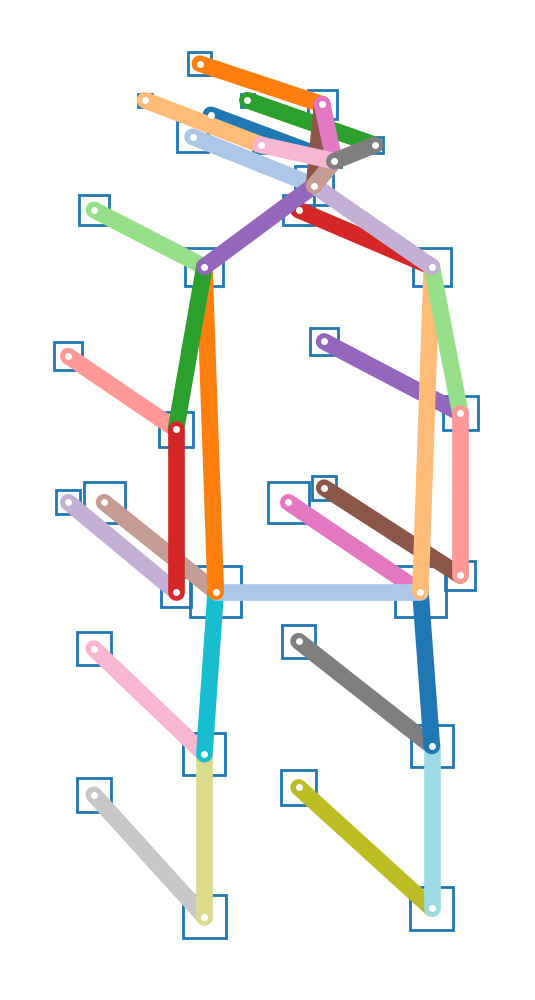
\includegraphics[height=0.2\textheight]{Figures/skeleton_forward2.png}
    \caption{Vizualizace  sledování osoby mezi dvěma snímky v OpenPifPaf \cite{openpifpaf}}
    \label{fig:pipaf-tracking}
\end{figure}

U OpenPifPaf je k dispozici výběr několika páteřních modelů, jako je ResNet50
či ShuffleNet v různých variantách a velikostech. Můžeme tak zvolit model,
který je kompromisem mezi výkonem a přesností, v závislosti na konkrétních
požadavcích aplikace.

\subsection{MediaPipe – BlazePose}

MediaPipe je framework vyvinutý společností Google, umožňující jednoduchou
integraci různých technik strojového učení. Obsahuje různé algoritmy pro řešení
úloh jako detekce objektů, segmentace či detekce klíčových bodů (tváře či
pózy). MediaPipe je optimalizován pro mobilní zařízení a webové aplikace.
Detekce pózy v tomto frameworku je postavená na algoritmu BlazePose.

BlazePose implementuje přístup shora dolů, detekuje tedy nejprve RoI, ve
kterých detekuje osobu a její pózu. Nativně podporuje pouze jednu osobu ve
snímku. Ve videu ale v rámci optimalizace neprovádí detekci RoI pro každý
snímek, pouze pokud v aktuální RoI již není detekována osoba. Výhodou tohoto
algoritmu je, že detekuje 33 bodů v postavě, což je podstatně více, než většina
ostatních algoritmů, umožňuje tak přesnější analýzu některých situací, např.
podle natočení tváře, dlaní či stop.

Framework MediaPipe implementuje BlazePose spolu s detekcí více osob (použije v
první fáze detektor objektů) i sledování. Výhodou tohoto frameworku je jeho
kontinuální vývoj a jednoduchost integrace. Nevýhodou ale je, že pro systémy
Windows není implementována podpora GPU. Jelikož náš výsledný produkt bude
spouštěn primárně na Windows zařízeních, je pro nás tato vlastnost rozhodující.
Model je dostupný v třech velikostních variantách: $Lite$, $Full$ a $Heavy$.

\subsection{YOLO}

Od vydání YOLOv7 v roce 2022 integruje framework YOLO i detekci pózy. Oficiální
článek Chien-Yao Wanga et al. \cite{yolov7}. sice neobsahoval tuto funkčnost,
ale oficiální implementace zahrnula i implementaci YOLO-Pose \cite{yolo-pose}.
Obecně detekce pózy v YOLO kombinuje přístup shora dolů a zdola nahoru.
Algoritmus sice vyhledává klíčové body spolu s bounding boxy osob, nicméně vše
v jednom kroku. Samotná detekce klíčových bodů využívá regresi, což
zjednodušuje proces trénování, jelikož není třeba tvořit heatmapy.

Architektura použita v YOLO-Pose se ale liší od architektury používané v
pozdějších verzích. V YOLO-Pose jsou na konci řetězce umístěny hlavy pro různá
měřítka, jejich výstupem jsou bounding boxy a klíčové body, oba tvořené spolu.
V pozdějších verzích je architektura YOLO koncipována universálněji pro různé
úlohy. Obsahuje tak tři fáze\cite{yolov11}: páteř (ang. backbone), která
extrahuje mapu příznaků, krk (ang. neck), který přizpůsobuje mapu příznaků pro
různá měřítka, a hlavy (ang. head), které paralelně zpracovávají výstupy pro
různé úlohy, viz obrázek \ref{fig:yolov11} . Bounding box a klíčové body jsou
tedy sice generovány paralelně a teoreticky nezávisle, nicméně s ohledem na
proces trénování a postprocessing se v praxi navzájem výrazně ovlivňují.

\begin{figure}[]
    \centering
    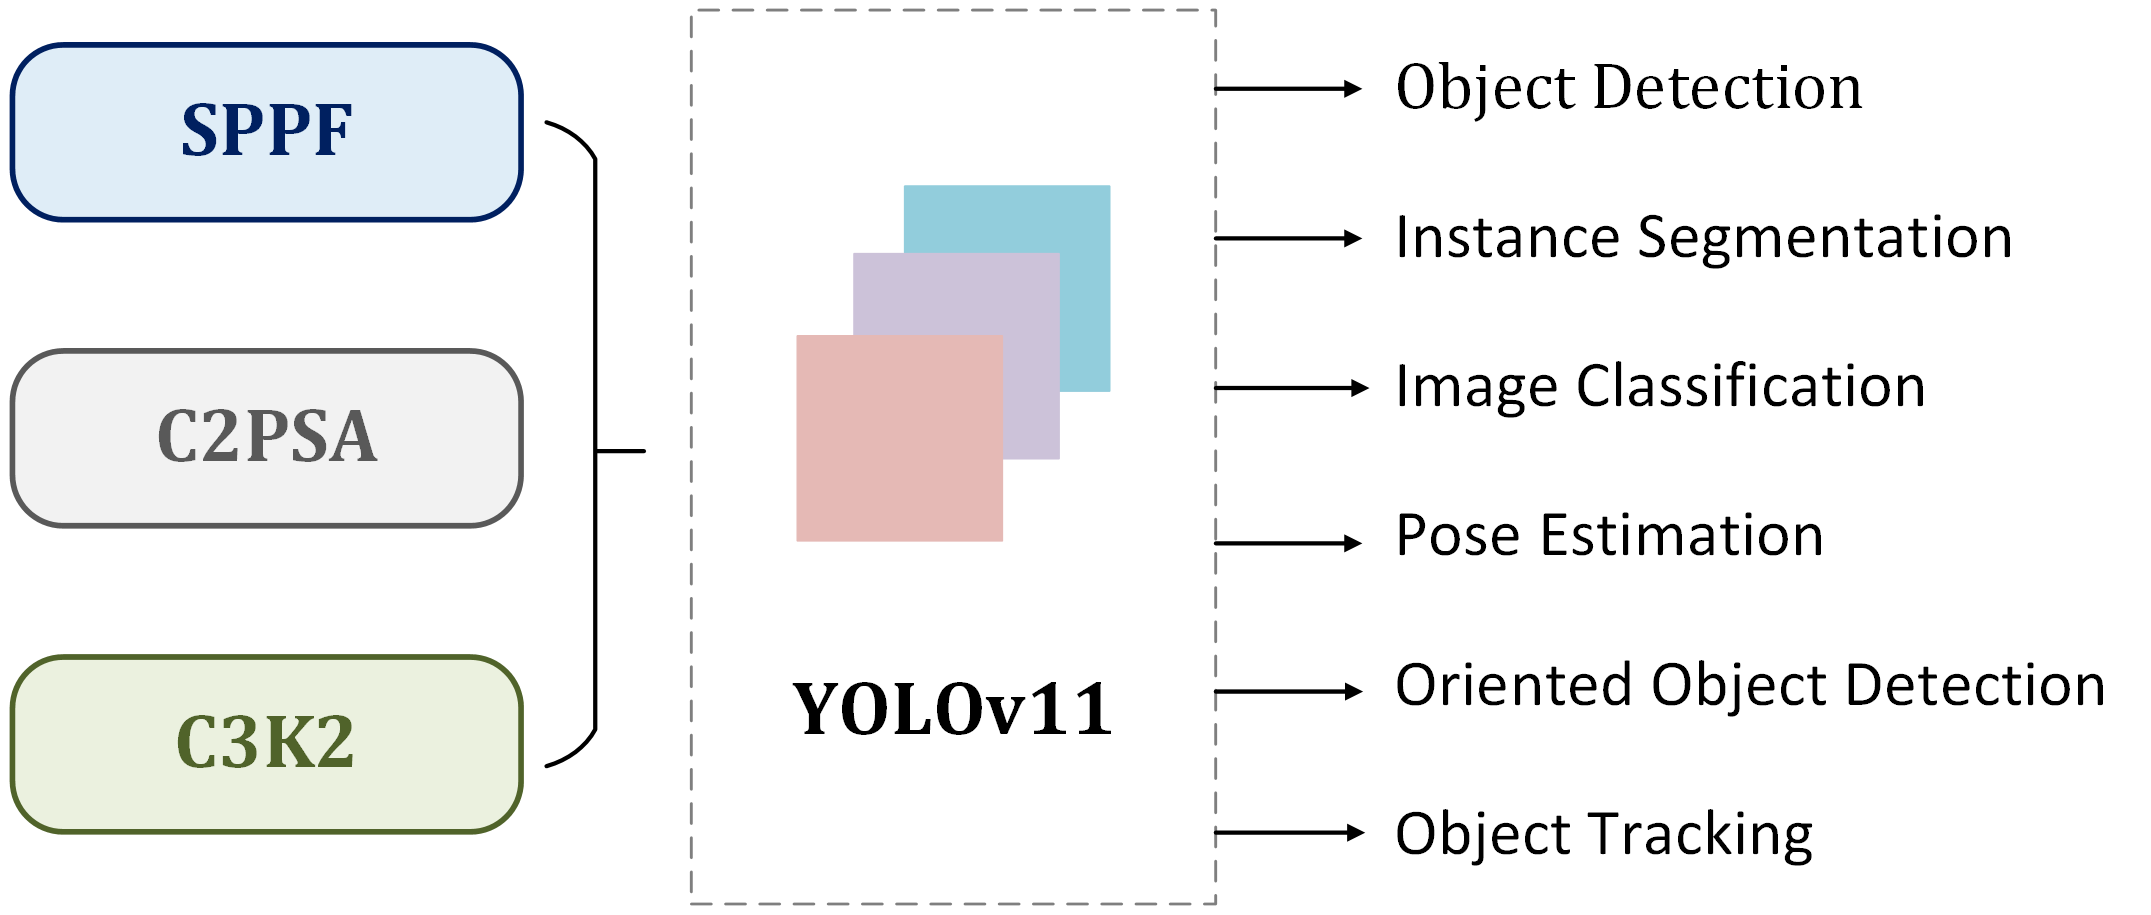
\includegraphics[height=0.2\textheight]{Figures/yolo_v11.png}
    \caption{Architektura YOLOv11 \cite{yolov11}}
    \label{fig:yolov11}
\end{figure}

Nejnovější verze YOLO také podporují kombinaci detekce klíčových bodů a
sledování osob. Model tedy kromě klíčových bodů vrací ID dané osoby, pomocí
kterého můžeme spojit danou postavu s předchozími snímky. Můžeme tak efektivně
analyzovat pohyby jednotlivých osob.

Jednou z výhod framevorku YOLO, zejména verzí vyvíjených firmou Ultralytics, je
široká škála velikostí modelů. Každý model je dostupný v pěti variantách:
$Nano$, $Small$, $Medium$, $Large$, $Xlarge$.

\subsection{Torchvision}

Torchvision je knihovna, která je součástí frameworku PyTorch. Obsahuje různé
nástroje pro strojové vidění, jako je detekce objektů či segmentace. Její
součástí je i předtrénovaný model pro detekci pózy, který implementuje
algoritmus Keypoint R-CNN \cite{keypoint-rcnn}.

Algoritmus Keypoint R-CNN je založen na stejné myšlence jako Mask R-CNN
\cite{mask-r-cnn}, a tedy rozšíření Faster R-CNN o další hlavu, která v případě
Mask R-CNN provádí segmentaci, v případě Keypoint R-CNN detekuje klíčové body.
V algoritmu je také upravená pooling vrstva, která zajišťuje, že se výstupy
algoritmu shodují s vstupy s přesností pixelu.

Tuto implementaci budeme testovat zejména z důvodu její jednoduchosti použití a
integrace do frameworku PyTorch, který budeme používat i v další části řešení.
Na druhou stranu máme oproti jiným frameworkům, jako je YOLO či MediaPipe, k
dispozici pouze jeden model, nikoliv více velikostních variant.

\section{Testování a porovnání vybraných algoritmů pro detekci pózy}

Pro testování jsme vybrali čtyři algoritmy pro detekci pózy, zejména na základě
jejich jednoduchosti implementace, aktualizované podpory a požadovaných funkcí.
Budeme tedy testovat algoritmy Torchvision, OpenPifPaf, MediaPipe BlazePose a
YOLO v nejnovější verzi 11. Testy byly provedeny na 25 videích ze stejného
datasetu jako byl použit později pro trénování algoritmu pro analýzu klíčových
bodů. Testování probíhalo na počítači s procesorem Intel Core i7, 32 GB RAM a
grafickou kartou NVIDIA GeForce RTX 3080 s 10 GB VRAM.

Algoritmy Torchvision a OpenPifPaf byly testovány s použitím GPU, MediaPipe
pouze s využitím CPU, jelikož nemá podporu GPU v prostředí Windows. Algoritmus
YOLO jsme testovali na GPU a CPU, abychom porovnali jeho výkon v různých
podmínkách. Algoritmus YOLO jsme také vyzkoušeli na GPU s využitím funkce
sledování.

Výstupem testování pro daný algoritmus a jeho variantu je průměrná doba
zpracování jednoho snímku a videa s vykreslením klíčových bodů. Tyto videa nám
dovolují ověřit schopnost detekce klíčových bodů v různých situacích a její
přesnost.

Podíváme se nyní na výsledky testování jednotlivých algoritmů. Pro každý
algoritmus porovnáme jednotlivé varianty s ohledem na rychlost a přesnost a
vyhodnotíme jeho výhody či nevýhody oproti ostatním algoritmům. Nakonec zvolíme
model, který použijeme v další části vývoje.

\subsection{Výkonové požadavky}
\label{sec:performance_requirements}

Při výběru algoritmu musíme s ohledem na práci v reálném čase brát v úvahu
zejména výkon detekčního algoritmu. Bezpečnostní kamery mají obvykle snímkovou
frekvenci od 15 do 30 snímků za sekundu (FPS), ideální by tedy bylo, aby
konečný program byl schopen pracovat s frekvencí alespoň 30 FPS. Zároveň se
předpokládá, že v prostředí, kde bude program nasazen, bude dostupná grafická
karta.

V této fázi jsme již zkoušeli trénování neuronové sítě pro klasifikaci pózy, a
ověřili jsme, že i v případě hlubších a komplexnějších sítí dosahujeme doby
inference v řádu nižších jednotek milisekund. Hlavní vliv na výslednou rychlost
programu tedy bude mít hlavně detekční algoritmus, který musí zpracovávat
mnohem větší objem dat – stovky tisíc až miliony pixelů oproti např. 17
klíčovým bodům v případě klasifikačního algoritmu.

\subsection{OpenPifPaf}

Algoritmus OpenPifPaf jsme zkoušeli v několika variantách, postavených na síti
\textit{ResNet 50} a \textit{ShuffleNet V2} \cite{shufflenetv2}. V tabulce
\ref{tab:openpifpaf_performance} vidíme, že většina variant ani zdaleka
nedosahuje požadovaného výkonu.

Tento algoritmus je poměrně robustní z pohledu světelných podmínek a rozlišení
či rozmazaní obrazu, jinak ale dosahuje nejhorší přesnosti ze všech testovaných
algoritmů. Kromě nedetekování části těla, které nejsou vidět (jsou např.
schovány za jinou částí těla), totiž často nedetekuje člověka vůbec, nejčastěji
pak když člověk padá nebo leží, což jsou situace pro nás stěžejní. Hlavně tento
problém vystupuje ve variantě $resnet50$ a $shufflenetv2k16$, jsou tak pro nás
nepoužitelné. Varianty $shufflenetv2k30$ a $tshufflenetv2k30$ by sice s ohledem
na kvalitu výsledků použitelné byly, nicméně je jejich výkon příliš nízký.

\begin{table}[htbp]
    \centering
    \caption{Porovnání výkonu modelu OpenPifPaf}
    \label{tab:openpifpaf_performance}
    \begin{tabular}{|l|l|l|l|}
        \hline
        \textbf{Verze}   & \textbf{inference [ms]} & \textbf{Frekvence [FPS]} \\
        resnet50         & 49,2                    & 20.324                   \\ \hline
        shufflenetv2k16  & 31,3                    & 31.910                   \\ \hline
        shufflenetv2k30  & 58,6                    & 17.070                   \\ \hline
        tshufflenetv2k30 & 70,0                    & 14.281                   \\ \hline
    \end{tabular}
\end{table}

\subsection{MediaPipe BlazePose}

Algoritmus BlazePose z knihovny MediaPipe jsme testovali ve třech variantách:
$Lite$, $Full$ a $Heavy$. Ve všech variantách tento algoritmus dosahoval velmi
přesných výsledků, asi nejlepších ze všech testovaných algoritmů. Na rozdíl od
jiných algoritmů totiž, pokud detekoval osobu, vždy velmi přesně označil
všechny její klíčové body, v rámci možností i ty, které byly hůře viditelné
(např. schovány za jinou částí těla). Na obrázku \ref{fig:ym_comparison} je
vidět rozdíl v přesnosti detekce klíčových bodů mezi nejmenší variantou
BlazePose a druhou největší variantou YOLO, kdy BlazePose dosahuje mnohem větší
přesnosti, v tomto příkladě zejména co se týče detekce nohou.

\begin{figure}
    \centering
    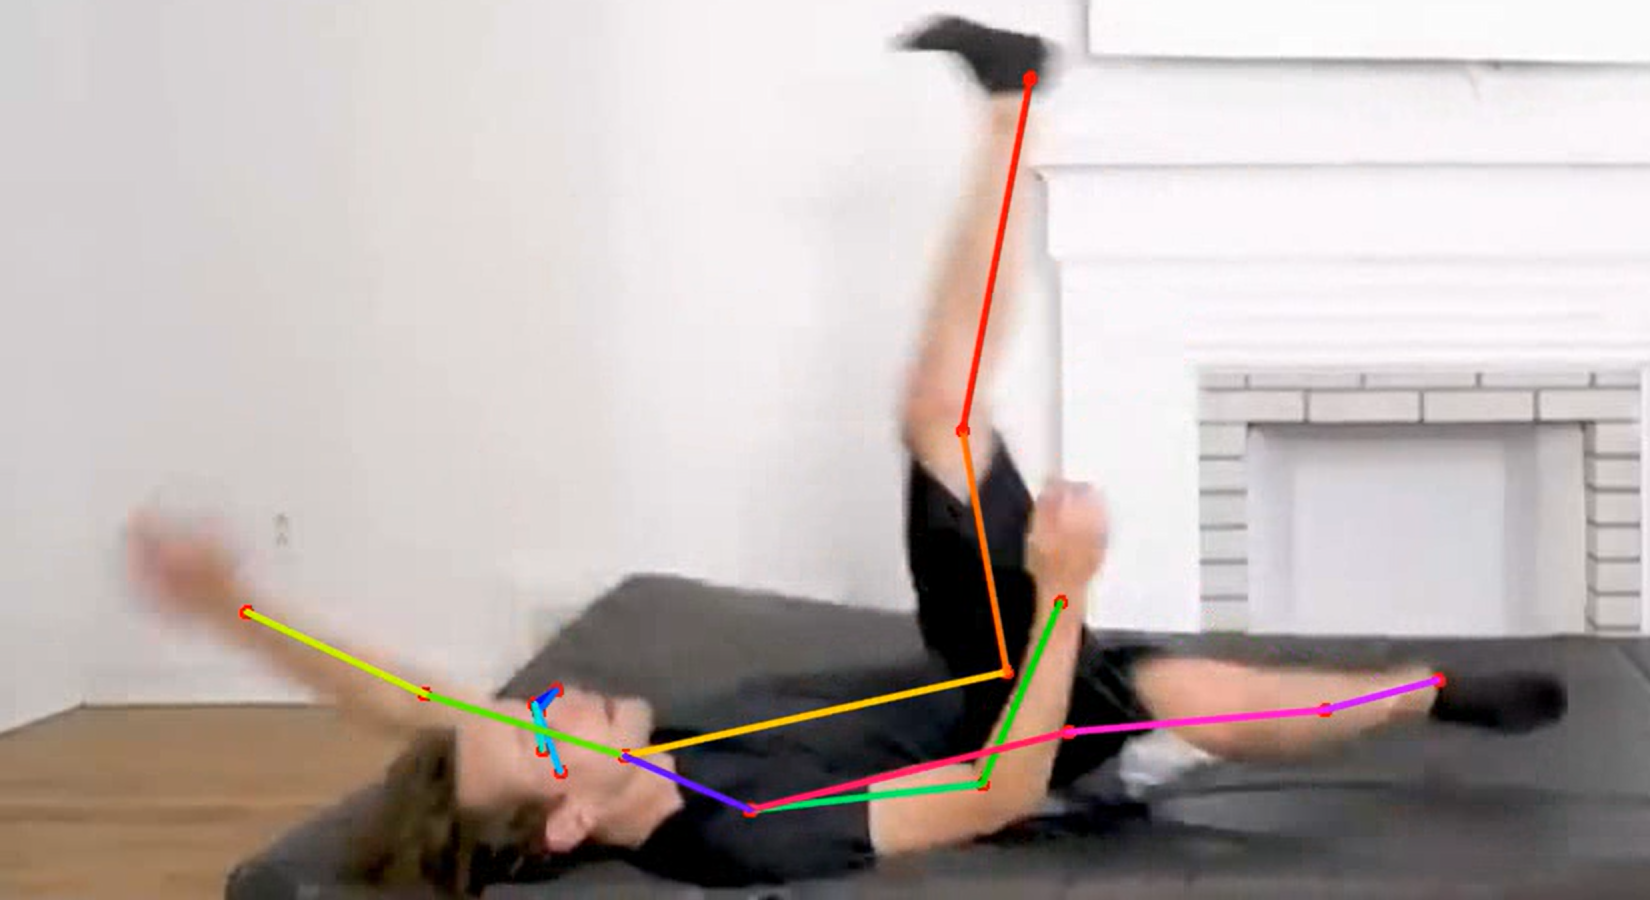
\includegraphics[width=0.4\textwidth]{Figures/pose_tests/mh1.png}
    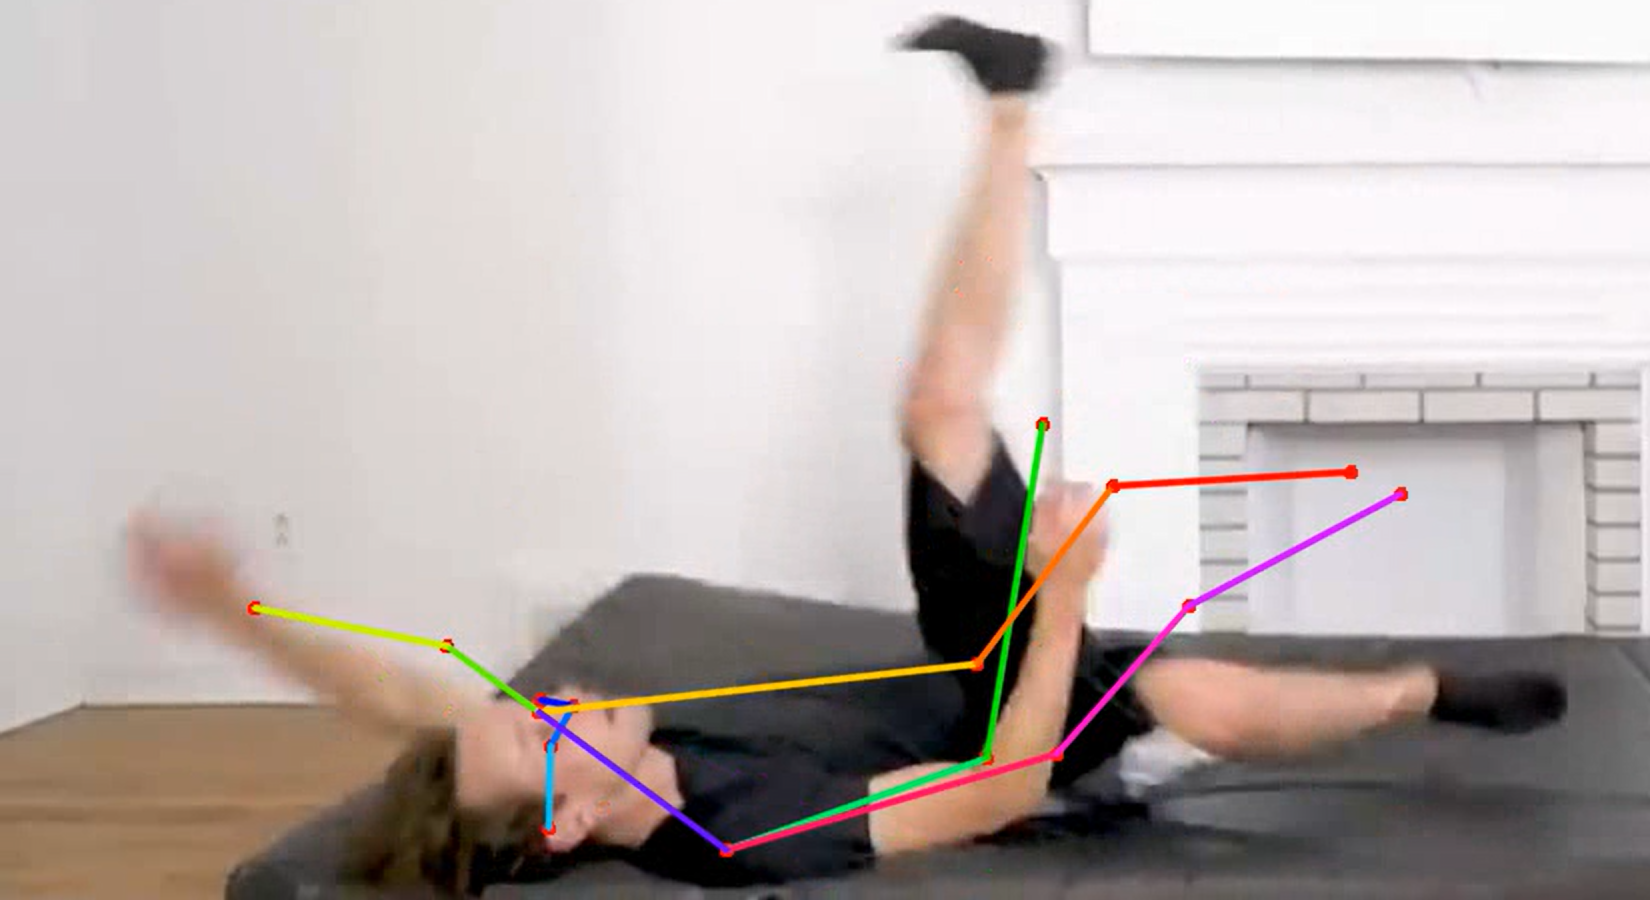
\includegraphics[width=0.4\textwidth]{Figures/pose_tests/yl1.png}
    \caption{Porovnání přesnosti \textit{MediaPipe Lite} (vlevo) a \textit{YOLO Large} (vpravo)}
    \label{fig:ym_comparison}
\end{figure}

S ohledem na to, že nemáme k dispozici grafickou akceleraci, je jeho výkon
velmi dobrý, viz tabulka \ref{tab:mediapipe_performance}. Verze $Lite$ a $Full$
by tak mohla být v našem řešení použitelná, což by nám také dávalo možnost
nasazovat výsledný program v mobilních zařízeních či jiných systémech bez
grafické karty.

\begin{table}[htbp]
    \centering
    \caption{Porovnání výkonu modelu MediaPipe BlazePose}
    \label{tab:mediapipe_performance}
    \begin{tabular}{|l|l|l|l|}
        \hline
        \textbf{Verze} & \textbf{inference [ms]} & \textbf{Frekvence [FPS]} \\
        \hline
        lite           & 25.5                    & 39.239                   \\ \hline
        full           & 30.9                    & 32.405                   \\ \hline
        heavy          & 68.2                    & 14.655                   \\ \hline
    \end{tabular}
\end{table}

Algoritmus si ale velice špatně radí s horšími světelnými podmínkami či menším
rozlišením obrazu. Ve většině případů sice detekuje klíčové body velmi přesně,
pokud je ale osoba hůř viditelná, nedetekuje ji vůbec. Tento problém se
projevuje ve všech variantách podobně. Jelikož bude náš výsledný program
nasazován spíše právě v podmínkách s horším osvětlením a ve větší vzdálenosti
od osob, pravděpodobně se pro naši aplikaci nebude hodit.

\subsection{Torchvision Keypoint R-CNN}

Torchvision Keypoint R-CNN nedosáhla ani dostatečného výkonu, viz tabulka
\ref{tab:torchvision_performance}, ani kvalitních výsledků. Podobně jako
\textit{OpenPifPaf} má totiž problém, když osoba padá anebo leží. V tomto
případě osobu často detekuje, ale naprosto ztrácí přesnost detekovaných
klíčových bodů, nejčastěji záměnou jednotlivých bodů, viz obrázek
\ref{fig:torchvision_bad}. Zároveň oproti BlazePose nemá takový problém d
horšími světelnými podmínkami a menším rozlišením obrazu.

\begin{figure}[]
    \centering
    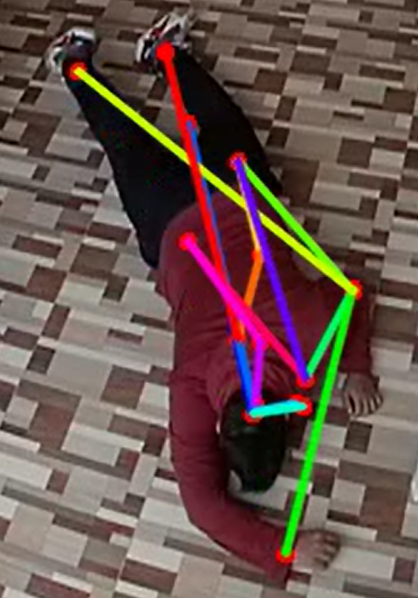
\includegraphics[width=0.2\textwidth]{Figures/pose_tests/torchvision_bad.png}
    \caption{Příklad špatné detekce bodů v modelu Torchvision Keypoint R-CNN}
    \label{fig:torchvision_bad}
\end{figure}

\begin{table}[htbp]
    \centering
    \caption{Výkon modelu Torchvision Keypoint R-CNN}
    \label{tab:torchvision_performance}
    \begin{tabular}{|l|l|}
        \hline
        \textbf{inference [ms]} & \textbf{Frekvence [FPS]} \\
        \hline
        50.3                    & 19.897                   \\ \hline
    \end{tabular}
\end{table}

\subsection{YOLO}

Algoritmus YOLO ve verzi 11 jsme testovali v pěti variantách: $Nano$, $Small$,
$Medium$, $Large$ a $Xlarge$. Všechny varianty byly testovány na GPU i CPU.

V tabulce \ref{tab:yolo_performance} vidíme, že na CPU dosahuje tento
algoritmus poměrně špatných výsledků. Jediný použitelný by pro nás mohl být v
takové situaci model $Nano$. YOLO je ale velice kvalitně optimalizováno pro
grafické karty, můžeme tak pozorovat, že na GPU je výkon výrazně vyšší. Pro
naše potřeby by tak byly použitelné prakticky všechny varianty.

Jelikož pro analýzu více osob v jednom snímku je potřeba, zejména v případě
použití rekurentní neuronové sítě, jednotlivé osoby od sebe oddělit a
identifikovat i mezi snímky, bude pro nás velmi užitečná funkce sledování
objektu. Proto jsme otestovali algoritmus YOLO i s touto funkcí. Jak je vidět v
tabulce \ref{tab:yolo_performance}, je výkon sice horší než bez sledování,
pořád ale tři menší varianty dosahují frekvence větší než $30$ FPS.

\begin{table}[htbp]
    \centering
    \caption{Porovnání výkonu modelu YOLO}
    \label{tab:yolo_performance}
    \begin{tabular}{|c|l|l|l|}
        \hline
                                           & \textbf{Verze} & \textbf{inference [ms]} & \textbf{Frekvence [FPS]} \\
        \hline\hline
        \multirow{3}{*}{CPU}               & nano           & 32.5                    & 30.749                   \\ \cline{2-4}
                                           & small          & 53.9                    & 18.563                   \\ \cline{2-4}
                                           & medium         & 114.1                   & 8.763                    \\ \cline{2-4}
                                           & large          & 143.4                   & 6.973                    \\ \cline{2-4}
                                           & xlarge         & 833.2                   & 1.200                    \\ \hline\hline
        \multirow{3}{*}{GPU}               & nano           & 15.1                    & 66.323                   \\ \cline{2-4}
                                           & small          & 15.2                    & 65.972                   \\ \cline{2-4}
                                           & medium         & 17.4                    & 57.500                   \\ \cline{2-4}
                                           & large          & 24.4                    & 41.026                   \\ \cline{2-4}
                                           & xlarge         & 24.4                    & 41.005                   \\ \hline\hline
        \multirow{3}{*}{GPU se sledováním} & nano           & 27.4                    & 36.500                   \\ \cline{2-4}
                                           & small          & 27.7                    & 36.148                   \\ \cline{2-4}
                                           & medium         & 29.5                    & 33.882                   \\ \cline{2-4}
                                           & large          & 37.5                    & 26.664                   \\ \cline{2-4}
                                           & xlarge         & 40.5                    & 24.695                   \\ \hline
    \end{tabular}
\end{table}

Všechny varianty algoritmu YOLO dosahují poměrně kvalitních výsledků. I v
horších světelných podmínkách vždy detekují osobu, a víceméně přesně určí její
klíčové body. Obecně je ale vidět, že je model trochu méně robustní (než např.
MediaPipe) v situacích, kdy není dobře vidět některá končetina – je třebas
schovaná za jinou částí těla, anebo ve specifických pózách – např. když je
osoba v dřepu nebo je v obraze natočená vzhůru nohama. V takovýchto případech
dosahuje menší přesnosti pro jednotlivé body – detekuje jiné natočení končetiny
nebo v extrémních případech špatně vyhodnotí natočení celé postavy. Špatně
viditelné části těla pak často vůbec nedetekuje.

Z pohledu přesnosti je zde výrazně vidět vliv velikosti modelu na přesnost
detekce. Varianta $Nano$ ve výše zmíněných situacích někdy detekuje body zcela
špatně, a je tak prakticky nepoužitelná. Varianta $Small$ je znatelně lepší,
pořád ale v horších podmínkách vyhodnocuje mnoho části těla špatně – např.
zamění nohy. Varianta $Medium$ je už výrazně lepší. Není sice ideální, ve valné
většině ale vyhodnotí všechny části těla správně i když ne z přesností několika
pixelů. Varianty $Large$ a $Xlarge$ jsou pak už velmi přesné, projevuje se to
ale znatelně menší rychlostí.

\begin{figure}
    \centering
    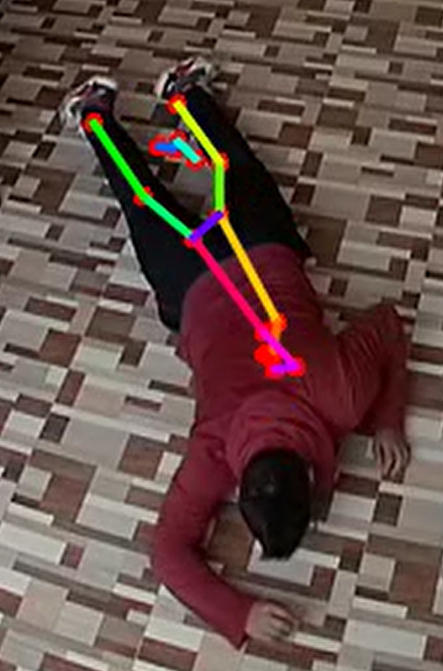
\includegraphics[width=0.18\textwidth]{Figures/pose_tests/y_n.png}
    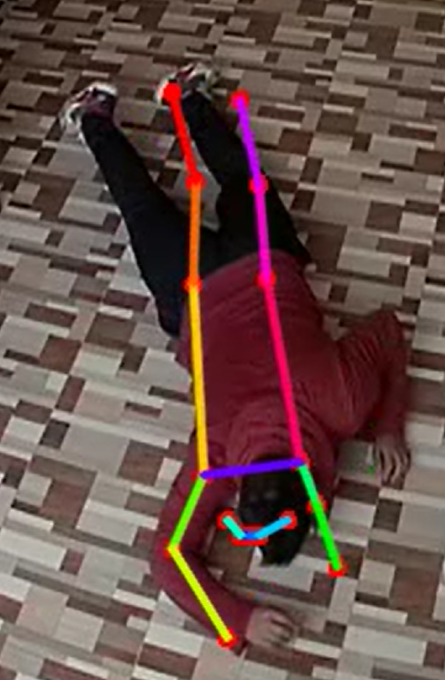
\includegraphics[width=0.18\textwidth]{Figures/pose_tests/y_s.png}
    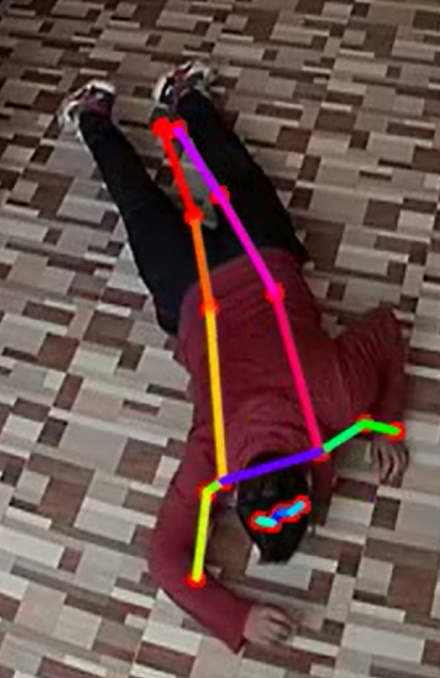
\includegraphics[width=0.18\textwidth]{Figures/pose_tests/y_m.png}
    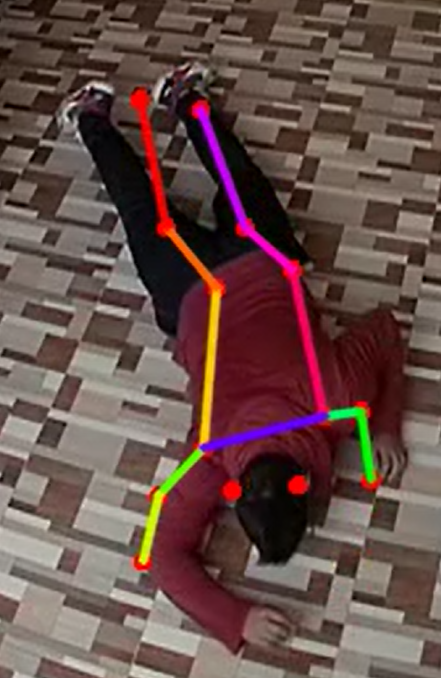
\includegraphics[width=0.18\textwidth]{Figures/pose_tests/y_l.png}
    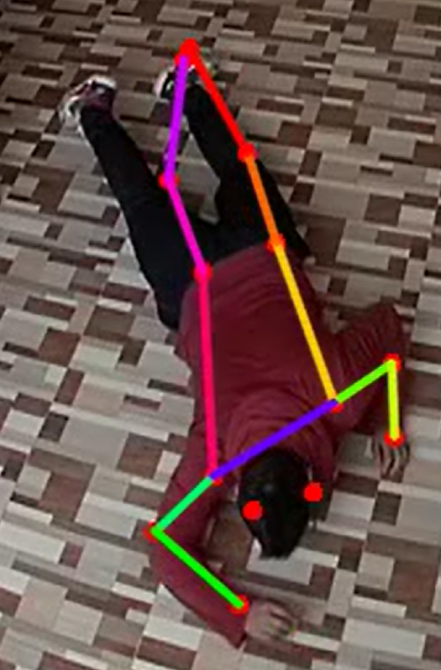
\includegraphics[width=0.18\textwidth]{Figures/pose_tests/y_x.png}
    \caption{Porovnání přesnosti variant modelu YOLO v situaci s netypickým natočením postavy. Zleva: $Nano$, $Small$, $Medium$, $Large$, $Xlarge$}
    \label{fig:y_comparison}
\end{figure}

Je zajímavé pozorovat, že i když je algoritmus BlazePose v mnoha situacích
mnohém přesnější, než i větší varianty YOLO, viz obrázek
\ref{fig:ym_comparison}, při horší viditelnosti, kdy i nejmenší varianty YOLO
detekují osobu, BlazePose zcela selhává. Ve snímku na obrázku
\ref{fig:y_comparison} například nedetekoval BlazePose osobu vůbec.

\subsection{Shrnutí a výběr modelu}

Z našeho testování jsme zjistili, že modely OpenPifPaf a Torchvision jsou
natrénované spíše pro detekci postavy, když je osoba v běžnějších pózách, jako
je ve stoje či chůze. Stejně i u menších variant YOLO přesnost prudce klesá v
méně typických pózách či natočeních v obraze. Jelikož ale je naše práce
postavena právě na detekování více netypické postavy, je pro nás důležité
detekovat pozici ve všech situacích.

Naopak algoritmus BlazePose je velmi přesný, strádá ale při horší viditelnosti
osoby. Nehodí se tak pro naše využití s kamerami s horším rozlišením a vysokou
vzdáleností od osob. Ostatní algoritmy v tomto ohledu jsou mnohem robustnější,
nejlépe si s horšími podmínkami poradí algoritmus YOLO.

Optimální cesta se tedy zdá být algoritmus YOLO ve verzi medium, kdy dosahuje
dostatečné rychlosti i při sledování osob, zároveň dostatečně přesně detekuji
pózy ve všech pozicích i podmínkách. Pokud bychom nevyužívali pro analýzu pózy
rekurentní neuronovou síť, nemuseli bychom používat funkci sledování a mohli
bychom tak použít i větší variantu YOLO, což by mohlo zlepšit přesnost detekce.

\endinput

\chapter{Implementace klasifikační neuronové sítě}
\label{chap:ClassificationImplementation}

Problematika vyhodnocování je velmi široká a přináší mnoho problémů. Ostatně i
člověk někdy může špatně interpretovat chování druhé osoby. Například pokud
někdo skáče do postele či jinak prudce lehá, může to vypadat jako nebezpečná
situace. Stejně se v počítačovém vidění nevyhneme falešným poplachům, nicméně
se budeme snažit zapojit různé techniky pro zlepšení přesnosti našeho
detektoru.

Naším úkolem je nyní vytvořit algoritmus, který pro danou pózu (reprezentovanou
klíčovými body), resp. sekvenci takových póz (získané pro jednu osobu ze
sekvence snímků), určí, zda se jedná o situaci pádu, či nikoliv. Tento
algoritmus bude přijímat vždy pózu jedné osoby, funkcionalita pro více osob
bude řešená později.

V kapitole \ref{chap:Pose} jsme pro detekci klíčových bodů zvolili model
\textit{YOLO pose}. Ten je předtrénovaný na datasetu \textit{COCO}, který pro
lidské pózy definuje 17 klíčových bodů v dvourozměrném prostoru. To udává
velikost vstupu do našeho klasifikačního algoritmu. Navrhneme tedy a
natrénujeme neuronovou síť, jejíž vstupem bude 17 2D klíčových bodů - tedy 34
čísel - a výstupem bude klasifikace třídy pózy - \textit{normální} a
\textit{upadl}.

V této kapitole se zaměříme na implementaci klasifikačního algoritmu pro
analýzu pózy. Nejdříve se podíváme na použité technologie a knihovny, které nám
pomohou s vývojem. Poté rozebereme možné architektury sítě a ukážeme, jak byly
implementovány. Dále se zaměříme na návrh vnitřní struktury u těchto
architektur, zkusíme je natrénovat v různých konfiguracích a vybereme
nejoptimálnější řešení. Nakonec toto řešení otestujeme na testovacím datasetu.

\section{Použité technologie}

\subsection{PyTorch}

Celý projekt byl vyvíjen v prostředí skriptovacího jazyka Python. Samotný vývoj
neuronových sítí probíhal ve frameworku PyTorch. PyTorch je open-source
knihovna pro strojové učení, široce používaná například pro počítačové vidění
či zpracování přirozeného jazyka. Jeho hlavními funkcemi je práce s tenzory
podobnými jako v NumPy, ale s podporou silné akcelerace s využitím GPU, a vývoj
neuronových sítí postavený na vysokoúrovňových stavebních blocích s podporou
automatické derivace pro počítaní gradientů.

Implementace neuronových sítí v PyTorch je velice jednoduchá a díky vysoké míře
abstrakce umožňuje se při vývoji soustředit na samotnou architekturu a design
sítě, nikoliv na detaily implementace. Pro vytvoření nové neuronové sítě stačí
vytvořit třídu, která bude dědit od základní třídy $nn.Module$, v konstruktoru
definovat jednotlivé vrstvy včetně různých regularizačních hyperparametrů. V
metodě $forward$ pak definujeme dopředný průchod sítě. Dále máme možnost
kontrolovat např. výpočet ztrátové funkce či metriky přesnosti.

PyTorch obsahuje také předpřipravené moduly pro GRU či LSTM sítě, včetně
vícevrstvých architektur. Pro tyto moduly definujeme velikost vstupu a velikost
skrytého stavu, dále můžeme definovat počet vrstev či dropout. Výstup z těchto
modulů je pak skrytý stav, který můžeme dále zpracovávat pomocí jednoduché
dopředné sítě pro predikci třídy.

\subsection{Lightning}
\label{sec:Lightning}

PyTorch Lightning je wrapper pro PyTorch, který dále usnadňuje vývoj
neuronových sítí. Stará se za nás o detaily procesu trénování, jako je správa
epoch, logování či optimalizace kroku učení (ang. learning rate). Podporuje
taky nativně práci s TensorBoard, což je logovací nástroj umožňující přehledné
sledování metrik během trénování, včetně grafického zobrazení ve webovém
prostředí.

Pro implementaci modelu vytvoříme třídu, která dědí z
$lightning.LightningModule$, a kromě konstruktoru, ve kterém inicializujeme
jednotlivé vrstvy, definujeme metody $training\_step$ (krok trénování),
$validation\_step$ - krok validace, $configure\_optimizers$ - definování
optimalizační techniky a $forward$, která definuje, jak signál prochází
jednotlivými vrstvami.

\section{Implementace vybraných architektur}
\label{sec:SelectedArchitectures}

Podíváme se nyní, jak jsme jednotlivé architektury implementovali, nezávisle na
jejich vnitřní struktuře a konfiguraci.

\subsection{Dopředná neuronová síť}

Nejjednodušší architekturou, kterou můžeme pro náš model použít, je dopředná
neuronová síť. Tento model pak bude klasifikovat jednotlivé pózy, aniž by znal
jejich kontext. Síť bude klasifikovat klíčové body pouze podle aktuální
lokalizace ve snímku, nikoliv podle pohybu.

Výhodou této architektury je jednoduchost, potažmo rychlost. Síť nepotřebuje
mnoho parametrů a oproti rekurentním sítím potřebuje pro evaluaci pouze jeden
dopředný průchod vrstvami sítě.

Další výhodou je jednoduchost trénování a používání. V případě více osob pro
samotnou klasifikaci pádu není nutné sledování osob. Můžeme jednoduše
klasifikovat všechny detekované pózy, aniž bychom řešili, které osobě patří.

Tato síť ale ve výsledku bude klasifikovat pózy pouze dle vzájemného umístění
jednotlivých klíčových bodů, potažmo délky končetin, nebude ale brát v úvahu
natočení postavy. To proto, že postavy ve snímku vystupují pod různým úhlem
natočení v závislosti na natočení kamery. Naopak síť, která je schopná sledovat
pohyb, bude schopna sledovat mj. i změnu natočení postavy a to bez ohledu na
natočení kamery.

Při použití této architektury jsou jako vstupní data použity klíčové body jedné
osoby z daného jednoho snímku. Trénovací data pak pouze přečteme z trénovacího
souboru a překonvertujeme je do formy tenzoru, konkrétně je zabalíme do
instance třídy $DataLoader$. Při použití ve výsledném programu předáme modelu
klíčové body každé detekované osoby v daném snímku.

Výstupem sítě je hodnota od $0$ do $1$, čísla od $0$ do $0.5$ jsou považována
za třídu \textit{normální}, zatímco čísla od $0.5$ do $1$ za třídu
\textit{upadl}.

Pro implementaci dopředné sítě v Pytorch Lightning jsme použili modul
$nn.sequential$, ve kterém definujeme postupné kroky průchodů sítě. $nn.Linear$
definuje vrstvu sítě včetně počtu neuronů předcházející a aktuální vrstvy. Dále
můžeme definovat aktivační funkci po dané vrstvě a regularizační techniky jako
je dropout či normalizace. Příklad implementace dopředné sítě je uveden v kódu
\ref{src:ffnn}. V tomto příkladě jsou definovány dvě vnitřní vrstvy o velikosti
$128$ a $32$ a výstupní vrstva s jedním neuronem. Mezi vrstvami je aplikována
normalizace a dropout $0.3$, jako aktivační funkce je použita ReLU.

\begin{lstlisting}[language=Python, label=src:ffnn, caption={Ukázka implementace Dopředné sítě v PyTorch Lightning}]
class KeypointClassifierFFNN(L.LightningModule):
    def __init__(self):
        super(KeypointClassifierFFNN, self).__init__()
        self.classifier = nn.Sequential(
            nn.Linear(34, 128),
            nn.BatchNorm1d(128),
            nn.ReLU(),
            nn.Dropout(0.3),
            nn.Linear(128, 32),
            nn.BatchNorm1d(32),
            nn.ReLU(),
            nn.Dropout(0.3),
            nn.Linear(32, 1),
        )
        self.criterion = nn.BCEWithLogitsLoss()
        self.accuracy = BinaryAccuracy(threshold=0.5)
        self.sigmoid = nn.Sigmoid()    
    def forward(self, x):
        x = self.classifier(x)
        return x
    def configure_optimizers(self):
        optimizer = optim.Adam(self.parameters(), lr=1e-4)
        return optimizer
    def training_step(self, batch, batch_idx):
        input, target = batch
        output = self(input)
        loss = self.criterion(output, target.float())    
        self.log("train_loss", loss, on_epoch=True, on_step=False)
        return loss
    def validation_step(self, batch, batch_idx):
        data, target = batch
        output = self(data)
        loss = self.criterion(output, target.float())
        self.log('val_loss', loss, on_epoch=True, on_step=False)
        output = self.sigmoid(output)
        accuracy = self.accuracy(output, target.int())    
        self.log('val_accuracy', accuracy, on_epoch=True, on_step=False)
    return loss
\end{lstlisting}

Abychom mohli tuto síť efektivně trénovat, musíme umožnit jednoduchou změnu
konfigurace sítě. Třída $KeypointClassifierFFNN$ proto v konstruktoru přijímá
parametry \textit{layers} - pole čísel reprezentujících velikosti jednotlivých
vrstev, \textit{activation} - identifikátor vybrané aktivační funkce a
\textit{dropout} definující velikost dropoutu, viz kód \ref{src:ffnn_params}.
Jako ztrátovou funkci jsme použili křížovou entropii, tedy
$nn.BCEWithLogitsLoss()$, která je vhodná pro binární klasifikaci.

\begin{lstlisting}[language=Python, label=src:ffnn_params, caption={Parametrizace konfigurace dopředné sítě}] 
class KeypointClassifierFFNN(L.LightningModule):
    def __init__(self, layers, activation, dropout=0.3, device=None):
        super(KeypointClassifierFFNN, self).__init__()        
        classifier = nn.Sequential()
        for i in range(len(layers)-1):
            classifier.add_module(f'layer_{i}', nn.Linear(layers[i], layers[i+1]))
            classifier.add_module(f'batch_norm_{i}', nn.BatchNorm1d(layers[i+1]))
            classifier.add_module(f'activation_{i}', activations[activation])
            classifier.add_module(f'dropout_{i}', nn.Dropout(dropout))
        classifier.add_module(f'layer_{len(layers)-1}', nn.Linear(layers[-1], 1))
        self.classifier = classifier
        self.criterion = nn.BCEWithLogitsLoss()
        self.accuracy = BinaryAccuracy(threshold=0.5)
        self.layers = layers
        self.sigmoid = nn.Sigmoid()   
\end{lstlisting}

\subsection{GRU síť}

Jelikož pád je událost, nikoliv statická póza, mohlo by být optimálnější použít
algoritmus, který bude analyzovat nejenom aktuální pózu, ale sekvenci
posledních $n$ póz. Pro tento účel se nabízí rekurentní neuronové sítě. V
dnešní době je nejpoužívanější rekurentní architekturou GRU (Gated Recurrent
Unit).

Příklad implementace GRU sítě je uveden v kódu \ref{src:gru}, kde je definována
GRU jednotka s jednou vrstvou, velikosti vstupního vektoru $34$ a skrytým
stavem velikosti $128$, následována dvouvrstvou dopřednou plně propojenou sítí
ze $128$ neurony v první vrstvě a s jedním neuronem ve druhé vrstvě.

\begin{lstlisting}[language=Python, label=src:gru, caption={Ukázka implementace GRU sítě v PyTorch Lightning}]
    class KeypointClassifierGRU(lightning.LightningModule):
        def __init__(self):
            super(KeypointClassifierGRU, self).__init__()
            self.gru = nn.GRU(34, 128)              # GRU vrstvy
            self.classifier = nn.Sequential(        # Plně propojené vrstvy
                nn.Linear(128, 128),
                nn.ReLU(),
                nn.Dropout(0.3),
                nn.Linear(128, 1) )
            self.criterion = nn.BCEWithLogitsLoss ()    # Ztrátová funkce
            self.accuracy = BinaryAccuracy()            # Metrika přesnosti
        def forward(self, x):
            _, x = self.gru(x)
            x = x[-1]                               # Poslední skrytý stav
            x = self.classifier(x)
            return x
    
\end{lstlisting}

Část těchto hyperparametrů jsme opět parametrizovali, abychom mohli postupně
otestovat různé jejich kombinace a vyhodnotit jejich vliv na výkon modelu, viz
kód \ref{src:params}. Jedná se o velikost vstupního vektoru, velikost skrytého
stavu sítě GRU, počet vrstev GRU, velikost první plně propojené vrstvy,
velikost výstupní vrstvy (pro binární klasifikaci vždy $1$, potřebné pro
pozdější optimalizace) a dropout pro GRU i plně propojené vrstvy. Všechny tyto
hyperparametry budeme ladit v další části.

\begin{lstlisting}[language=Python, label=src:params, caption={Parametry konstruktoru třídy $KeypointClassifierGRU$ definující hyperparametry sítě}]
class KeypointClassifierGRU(L.LightningModule):
    def __init__(self, input_size=34, rnn_hidden_size=128, rnn_layers_count=2, fc_size=128, output_size=1, rnn_dropout=0.3, fc_dropout=0.3, device=None):
\end{lstlisting}

Stejně jako u předchozí architektury, jako ztrátová funkce byla použita binární
křížová entropie, tedy $nn.BCEWithLogitsLoss()$, která je vhodná pro binární
klasifikaci.

\subsection{LSTM síť}

Další populární rekurentní architekturou je LSTM (Long Short-Term Memory). Ta
je lepší pro delší sekvence, je to ale za cenu větší komplexity. Jak již bylo
vysvětleno, s nárůstem komplexity se zvyšuje riziko přetrénování, zejména při
nedostatku trénovacích dat. Vzhledem k množství trénovacích dat, které máme k
dispozici, se tak dá předpokládat, že trénování této sítě bude spíše méně
stabilní než v případě sítě GRU.

Implementace sítě LSTM se od GRU liší pouze použitím modulu $nn.LSTM$ místo
$nn.GRU$. Použití těchto modulů je v PyTorch velice podobné, pouze LSTM vrací
kromě skrytého stavu také stav buňky (dlouhodobou paměť), ten ale stejně
nevyužijeme. Pro síť LSTM budeme ladit stejnou množinu hyperparametrů, jako pro
GRU síť, abychom mohli porovnat jejich výkonnost.

\section{Návrh architektury a konfigurace sítě}

Nyní přistoupíme do samotného návrhu architektury a konfigurace sítě. Vybrané
architektury jsme natrénovali v různých konfiguracích a celý postup trénování
jsme zapisovali pomocí logovacího nástroje TensorBoard. Nyní na základě grafů
základních metrik, jako jsou ztrátová funkce či přesnost, zhodnotíme výkon
vybraných architektur, podíváme se, jaký mají jednotlivé hyperparametry vliv na
proces trénování a výsledný výkon. Nakonec vybereme nejoptimálnější variantu.

K hyperparametrům, které jsme zkoušeli, patří počet vrstev a jejich velikost a
velikost dropoutu. U dopředných sítí jsme navíc zkoušeli i různé aktivační
funkce, u rekurentních sítí pak velikost skrytého stavu. Pro optimalizaci váh
během trénování byl použit optimalizační algoritmus Adam \cite{adam}, jehož
výhodou je

\subsection{Dopředná neuronová síť}

Nejprve jsme zkoušeli natrénovat dopřednou neuronovou síť. Vyzkoušeli jsme od
dvou do čtyř vnitřních vrstev, ve velikostech od $32$ do $512$ neuronů, vždy
mocniny dvou. Pojďme postupně rozebrat jednotlivé hyperparametry a jejich vliv
na výkon modelu.

U dopředných sítí se nám nejlépe ověřila velikost dávky $4096$. Síť se lépe
trénovala s použitím normalizace (modul $nn.BatchNorm1d$) a dropoutu. Pro
většinu konfigurací byla velikost dropoutu $0.4$ nejoptimálnější.

Síť jsme zkoušeli trénovat s těmito vybranými aktivačními funkcemi: $ReLU$,
$Tanh$, $PReLU$ a $Mish$. $ReLU$ a $PReLU$ často dosahovaly podobných výsledků,
většinou ale nejlepších výsledků dosahovala $ReLU$. Příkladem je graf přesnosti
pro trénování sítě se třemi vnitřními vrstvami velikosti $128$, $64$, a $32$ na
obrázku \ref{graph:fnnactivations}.

\begin{figure}[]
    \centering
    \caption{Graf přesnosti na validačních datech v průběhu trénování dopředných sítí s různými aktivačními funkcemi}
    \label{graph:fnnactivations}
    \begin{tikzpicture}
        \begin{axis}[
                xlabel={Epochy},
                ylabel={Validační ztráta},
                ymin=70,
                grid=both,
                width=0.9\textwidth,
                height=0.4\textheight,
                legend pos=south east,
            ]
            \addplot[
                color=blue,
                mark=*,
                no markers
            ]
            table {Plots/relu.dat};
            \addlegendentry{ReLU}
            \addplot[
                color=green,
                mark=*,
                no markers
            ]
            table {Plots/prelu.dat};
            \addlegendentry{PReLU}
            \addplot[
                color=orange,
                mark=*,
                no markers
            ]
            table {Plots/tanh.dat};
            \addlegendentry{Tanh}
            \addplot[
                color=purple,
                mark=*,
                no markers
            ]
            table {Plots/mish.dat};
            \addlegendentry{Mish}
        \end{axis}
    \end{tikzpicture}
\end{figure}

Obecně větší sítě dosahovaly lepších výsledků - menší ztrátové funkce a vyšší
přesnosti na validačních datech, v jistém momentě jsme již ale začali narážet
na problém se stabilitou trénování. Nejoptimálnějších výsledků dosáhla síť se
třemi vrstvami o velikostech $128$, $64$ a $32$. Jak můžeme vidět na grafu
\ref{graph:deepffnn}, sítě s větší šířkou nebo hloubkou sice dosahují lepších
výsledků, začínají ale brzy výrazně kolísat. Zkoušeli jsme v těchto případech i
L2 regularizaci (parametr $weight\_decay$), to ale neřešilo problém. Pro
komplexnější sítě bychom pravděpodobně potřebovali větší množství dat.

Pojďme si tedy shrnout, jaká je pro nás nejoptimálnější konfigurace: použili
jsme tři vrstvy o velikostech $128$, $64$ a $32$, dropout $0.3$, normalizaci
mezi vrstvami, velikost dávky 4096 a aktivační funkci $ReLU$. Dosáhli jsme tak
validační ztráty $0.18$ a validační přesnosti 93.8%

\begin{figure}[]
    \centering
    \caption{Graf validační ztráty v průběhu trénování hlubších dopředných sítí }
    \label{graph:deepffnn}
    \begin{tikzpicture}
        \begin{axis}[
                xlabel={Epochy},
                ylabel={Validační ztráta},
                grid=both,
                width=0.9\textwidth,
                height=0.5\textheight,
                legend pos=north east,
                ymax=0.25,
            ]

            \addplot[
                color=blue,
                mark=*,
                no markers
            ]
            table {Plots/fnn_[34,128,64,32].dat};
            \addlegendentry{Velikosti vrstev: 128, 64, 32}
            \addplot[
                color=green,
                mark=*,
                no markers
            ]
            table {Plots/fnn_[34,256,128,32].dat};
            \addlegendentry{Velikosti vrstev: 256, 128, 32}
            \addplot[
                color=orange,
                mark=*,
                no markers
            ]
            table {Plots/fnn_[34,256,128,64,32].dat};
            \addlegendentry{Velikosti vrstev: 256, 128, 64, 32}
            \addplot[
                color=purple,
                mark=*,
                no markers
            ]
            table {Plots/fnn_[34,512,128,64,32].dat};
            \addlegendentry{Velikosti vrstev: 512, 128, 64, 32}
        \end{axis}
    \end{tikzpicture}
\end{figure}

\subsection{GRU síť}

Jak již bylo zmíněno, v oblasti jednodušších RNN jsou dnešním standardem GRU
sítě, sítě LSTM se používají zejména, pokud si GRU s problémem neradí, anebo je
vzhledem k problému důležité uchování dlouhodobých závislostí.

Stejnou taktiku zvolíme i my. Nejdříve otestujeme GRU sítě, a to pro několik
možností délky analyzované sekvence. To znamená, že pro každý snímek předáme
síti očekávanou třídu a sekvenci póz dané osoby z $n$ posledních snímků. Pak
vyzkoušíme síti předávat celou sekvenci póz dané osoby.

Naše GRU síť se skládá z několika vrstev GRU, konkrétně jsme zkoušeli trénovat
1 až 3 vrstvy, které následuje jedna plně propojená vrstva a výstupní vrstva.
Velikosti GRU vrstev jsme volili v rozsahu od 64 do 256, u plně propojené
vrstvy jsme volili mezi 32 a 128 neurony. Většinou jsme používali dávky o
velikosti $4096$, menší dávky velice destabilizovaly trénování.

Zjistili jsme, že na rozdíl od dopředných sítí, v případě GRU nejlepších
výsledků dosahovaly jednodušší sítě. Většina sítí s jednou GRU vrstvou tak
dosahovala poměrně stabilních výsledků. Nejvyšší přesnosti jsme pak dosáhli
sítí s jednou GRU vrstvou o velikosti $64$ a plně propojenou vrstvou o
velikosti $64$, s dropoutem 0.4 v plně propojené vrstvě. Co se týče dropout
mezi GRU vrstvami, bylo u hlubších sítí většinou dosaženo stabilnějších
výsledků s větší hodnotou dropoutu jako je 0.4, u jednovrstvých GRU sítí je
dropout nerelevantní, jelikož se aplikuje mezi vrstvami.

Sítě s více GRU vrstvami většinou než dosáhly optimálního výkonu, začaly
kolísat a ve validační ztrátě a přesnosti se objevovaly obrovské výkyvy.
Zkoušeli jsme větší dávky - $8162$, které sice stabilizovaly trénování při
stejném počtu epoch, jelikož se ale větší dávka loučí s pomalejším učením,
nedosahovaly takové přesnosti jako při dávkách velikosti $4096$. Pro dosažení
podobné přesnosti jsme tedy zkoušeli trénovat ve více epochách, tehdy ale brzy
docházelo k přetrénování.

RNN sítě obecně můžou přijímat sekvence libovolné délky, je ale efektivnější,
pokud je síť trénovaná na jednotné délce, tato délka sekvence je pak použitá i
v případě inferencí. Zkoušeli jsme tedy trénovat sítě na sekvencích o délce
$50$ a $100$ snímků, vyzkoušeli jsme i neomezenou délku sekvence, tedy modelu
předáváme klíčové body z celé sekvence snímků, na kterých byla daná osoba
detekována. Obecně jsme ale zjistili, že vždycky dosahují stabilnějších
výsledků sítě spíše s kratšími sekvencemi. Zůstali jsme tedy u sekvencí délky
$50$.

Naší nejlepší konfigurací GRU sítě je tedy jedna GRU vrstva o velikosti $64$,
následována plně propojenou vrstvou s $64$ neurony a dropoutem 0.4. Trénována
byla na sekvencích o délce $50$ snímků, s velikostí dávky $4096$ a s použitím
optimalizace Adam. Na obrázku \ref{graph:gru} pak můžeme vidět, že jsme dosáhli
trénovací ztráty $0.066$, validační ztráty $0.211$ a přesnosti $93.12\%$ .

\begin{figure}[] % 'htbp' controls figure placement (here, top, bottom, page)
    \centering
    \caption{Graf trénovací a validační ztráty (nahoře) a graf validační přesnosti v průběhu trénování výsledné sítě}
    \label{graph:gru}
    \begin{tikzpicture}
        \begin{axis}[
                % xlabel={Epochy},
                ylabel={Ztráta}, grid=both, width=0.9\textwidth, height=0.2\textheight, legend
                pos=north east, ymax=0.4, ]

            \addplot[
                color=green,
                mark=*,
                no markers
            ]
            table {Plots/gru_50_1_64_64_0.15_0.4_tloss.dat};
            \addlegendentry{Trénovací ztráta}
            \addplot[
                color=orange,
                mark=*,
                no markers
            ]
            table {Plots/gru_50_1_64_64_0.15_0.4_loss.dat};
            \addlegendentry{Validační ztráta}

        \end{axis}
    \end{tikzpicture}
    \begin{tikzpicture}
        \begin{axis}[
                xlabel={Epochy},
                ylabel={Validační přesnost},
                grid=both,
                width=0.9\textwidth,
                height=0.3\textheight,
                legend pos=north east,
                ymin=65,
            ]

            \addplot[
                color=green,
                mark=*,
                no markers
            ]
            table {Plots/gru_50_1_64_64_0.15_0.4_acc.dat};
            % \addlegendentry{Validační přesnost}

        \end{axis}
    \end{tikzpicture}
\end{figure}

\subsection{LSTM síť}

LSTM sítě jsme trénovali se stejnými hyperparametry a konfiguracemi jako sítě
GRU. Obecně se taky dá říct, že měly tyto parametry u obou architektur velice
podobný vliv na výsledky, a tedy to, co jsme napsali o GRU sítích, by se
většinou dalo napsat i o LSTM sítích. Taky měly nejlepší výsledky s jednou
vrstvou, podobně se projevovala délka sekvence, a obdobně byl většinou
optimální dropout velikosti $0.4$.

Obecně ale LSTM sítě byly mnohem méně stabilní, a prakticky v žádné konfiguraci
se nepodařilo natrénovat síť do požadované přesnosti, aniž by došlo k
přetrénování anebo by začala validační ztráta extrémně kolísat. Pravděpodobně
tedy nemáme dostatečný vzorek trénovacích dat pro trénování LSTM sítě. Taky,
sítě LSTM nejsou vhodny pro každou úlohu, spíše vynikají pro delší sekvence.

\section{Testování}
\label{sec:testing}

Vybrané modely jsme nakonec otestovali na testovacím datasetu. Ověříme jejich
přesnost a dobu inference. Konkrétně jsme testovali dopřednou neuronovou síť a
GRU síť, které v další kapitole, až bude naimplementovaný celý detektor pádu,
otestujeme na reálných datech.

\begin{table}[htbp]
    \centering
    \caption{Výsledky testování dopředné a GRU sítě}
    \label{tab:testing}
    \begin{tabular}{|c|c|c|cc|}
        \hline
        \multirow{2}{*}{} & \multirow{2}{*}{Ztráta} & \multirow{2}{*}{Přesnost} & \multicolumn{2}{c|}{Průměrná doba inference [ms]}         \\ \cline{4-5}
                          &                         &                           & \multicolumn{1}{c|}{  CPU  }                      & GPU   \\ \hline
        Dopředná síť      & 0.148                   & 94.43                     & \multicolumn{1}{c|}{0.207}                        & 0.647 \\ \hline
        GRU síť           & 0.138                   & 96.88                     & \multicolumn{1}{c|}{0.258}                        & 0.613 \\ \hline
    \end{tabular}
\end{table}

V tabulce \ref{tab:testing} vidíme, že obě sítě dosahují velmi dobrého výkonu.
Dopředná síť dosáhla přesnosti $94.43\%$ a ztráty $0.148$, zatímco GRU síť
dosáhla jak lepší přesnosti $96.88\%$, tak trošku menší ztráty $0.138$. Obě
sítě by tak mohly být použity pro detekci pádu, jelikož je ale pro klasifikační
úlohy v konečném řešení důležitější přesnost, GRU síť vypadá jako lepší
kandidát.

Z pohledu rychlosti jsou obě sítě natolik jednoduché, že ani nelze zaznamenat
výrazný rozdíl. Zároveň je velmi zajímavé, že je model na CPU asi třikrát
rychlejší než na GPU. Je to způsobeno tím, že je model malý, nelze tedy plně
využít potenciál paralelismu, navíc zpracováváme výstupy po jednom. Režie GPU
tedy převáží nad jejími výhodami. Ve všech případech se ale u doby inference
jedná o zlomky milisekund, ve výsledném programu doba prakticky zanedbatelná.

V další kapitole budeme implementovat detektor pádu, tedy program, který spojí
obě fáze detekce. Pomocí něj pak vyzkoušíme tyto dva modely, zejména s ohledem
na robustnost,
%
%
%
% TODO ::(
%
%
%
%
%
%
%
%
%
%
%
%
%

% \endinput
% %
% %
% %
% %
% %
% %
% %
% %
% %
% %
% %
% %
% %
% %
% %
% %
% %
% %
% %
% %
% %
% %
% %
% %
% %
% %
% %
% %
% %
% %
% %
% %
% %
% %
% %
% %
% %
% %
% %
% %
% %
% %
% %
% %
% %
% %
% \subsection{Vícetřídní klasifikace}

% Jak již bylo zmíněno (\ref{sec:TrainingData}), pro naše řešení potřebujeme
% detekovat pouze třídy \textit{normální} a \textit{upadl}, vyzkoušíme ale
% natrénovat i modely se třemi třídami - přidáme třídu \textit{padá}. Nemá smysl
% v našem případě implementovat takovou dopřednou neuronovou síť, jelikož
% klasifikuje snímky bez kontextu předchozích snímků.

% Budeme tedy navíc implementovat sítě GRU a LSTM, s velice podobnou topologií
% jako sítě s binární klasifikací. Hlavním rozdílem bude velikost výstupní
% vrstvy, jež bude rovna počtu tříd a použitá ztrátová funkce - nyní použijeme
% křížovou entropii. Výstup vícetřídní klasifikační sítě pak představuje pole
% pravděpodobností, že se jedná o danou třídu. Při inferenci pak použijeme
% jednotku softmax pro převod výstupu na číslo třídy.
% \chapter{Experimenty s topologiemi klasifikační sítě}
\label{chap:ClassificationExperiments}

% TODO


\chapter{Implementace kompletního řešení detekce pádu}
\label{chap:detectionProgram}

V této kapitole se zaměříme na implementaci celkového řešení detekce pádu,
který na základě postupně předávané sekvence snímků bude detekovat, zda došlo k
pádu. Jedná se tedy o spojení detekčního algoritmu, který ze snímku extrahuje
klíčové body všech osob, a klasifikačního algoritmu, který na základě těchto
bodů detekuje pád.

V našem případě tedy musíme spojit predikci modelu YOLO11-pose, a jednoho z
naších vybraných modelů (dopředná nebo GRU síť) pro klasifikaci pádu. Podíváme
se tedy nejprve krátce na práci ve frameworku YOLO. Následně se budeme zabývat
použitím dříve natrénovaných modelů. Zejména se zaměříme na implementaci s
využitím rekurentní architektury GRU, která přináší více výzev než dopředná
siť, s ohledem na nutnost uchovávání sekvence pro každého člověka zvlášť.
Nakonec program otestujeme s oběma klasifikačními modely na několika videích a
zhodnotíme jejich výkon.

\section{Sledování pózy s YOLO11}

V YOLO verze 11 máme kromě již zmíněné detekce objektů i klíčových bodů k
dispozici také další volitelné funkce. To, které funkce chceme využít,
definujeme vybraným modelem. V závislosti na něm pak při inferenci model vrací
patřičné hodnoty. Dostupné jsou tyto modely:
\begin{itemize}
    \item \textit{YOLO11<v>-seg } – detekce objektů – bounding boxů
    \item \textit{YOLO11<v>-cls } – detekce objektů, klíčových bodů a segmentace
    \item \textit{YOLO11<v>-pose} – detekce klíčových bodů
    \item \textit{YOLO11<v>-obb } – orientovaná detekce objektů – bounding boxy natočené dle natočení objektů
\end{itemize}

kde $<v>$ označuje velikost modelu – můžeme vybrat menší modely pro větší výkon
ale horší přesnost, anebo větší modely, které jsou sice velmi přesné, musíme
ale počítat s vysokými nároky na výkon. V našem případě jsme zvolili model
$YOLO11m-pose$. Pro inicializaci modelu musíme specifikovat cestu k němu, pokud
není nalezen, knihovna automaticky stáhne předtrénovaný model.

\begin{lstlisting}[language=Python, label=src:params, caption={Inicializace modelu $YOLO11m-pose$}]    
    from ultralytics import YOLO    
    pose_model = YOLO("./models_pose/yolo11m-pose.pt")
\end{lstlisting}

Dále můžeme každý z těchto modelů používat v několika režimech. Režim
specifikujeme tím, jakou metodu modelu použijeme. Pokud chceme model natrénovat
na vlastních datech, použijeme režimy \textit{trénování} (metoda $train()$) a
\textit{validace} (metoda $val()$). Pokud chceme používat již natrénovaný
model, máme k dispozici dva režimy: \textit{predikce} (přímé použití modelu,
např. $pose_model()$) pro vyhodnocení každého vstupního snímku zvlášť a
\textit{sledování} (metoda $track()$).

Režim \textit{sledování} vrací stejné informace jako režim \textit{predikce},
navíc ale sleduje pohyb objektů mezi jednotlivými snímky a přiřazuje jim $id$.
V našem případě tedy kromě bounding boxu a klíčových bodů dostaneme i $id$
každé osoby.

YOLO11 dokáže zpracovat širokou škálu vstupních dat, včetně videí, kdy nám je
vráceno pole výsledků, datových proudů (je třeba specifikovat příznak
$stream$), kdy nám je vrácen iterátor, nebo obrázků, kdy dostaneme výsledek pro
daný snímek. Pokud chceme použít režim \textit{sledování} na jednotlivé snímky,
musíme specifikovat příznak $persist$, který zajistí, že mezi jednotlivými
snímky bude uchovávána informace o sledovaných objektech. Zde můžeme vidět
použití metody $track()$ v našem programu (příznaky $show$ a $verbose$
specifikují, zda se má zobrazit výsledek každého snímku a zda má model do
konzoly vypisovat ladící informace)

\begin{lstlisting}[language=Python, label=src:params, caption={Použití sledování pomocí YOLO11}]
    results = self._pose_model.track(
        frame, show=False, verbose=False, persist=True)
\end{lstlisting}

\section{Struktura třídy FallDetector}

Třída $FallDetector$ slouží pro detekci pádu v sekvenci postupně předávaných
snímků. Můžeme ji tak použít jak pro analýzu uloženého videa, tak pro detekci
pádu v živém přenosu v reálném čase. Mezi jednotlivými snímky uchovává pro
každou osobu klíčové body z $x$ posledních snímků pro predikci na základě
sekvence snímků. Dále dle nastavení uchovává $n$ posledních snímků, popřípadě i
anotovaných, pro uložení videa včetně několika sekund před a po pádu. Pro
ukládání těchto informací používáme kolekci typu $deque$, která umožňuje
specifikovat její maximální délku, nerelevantní informace ze starších snímků
tedy budou automaticky odstraňovány.

V konstruktoru obdrží tato třída cestu k modelu YOLO (musí být inicializován
pro každou instanci zvlášť), model pro detekci pádu na základě klíčových bodů,
délku sekvence předávané tomuto modelu, a informace týkající se ukládání videí
s pády, jako jsou cesty k souborům a délka videa před a po pádu.

Pro práci s jednotlivými osobami používáme třídu $Person$, která uchovává
hlavně klíčové body z posledních snímků a $id$, dále také bounding boxy,
detekovaný stav a confidence score této detekce pro poslední snímek, kdy byla
osoba detekována. V případě, že daná osoba již není detekována, obsahuje
informaci, kolik snímků již není vidět pro vymazání osob, jež odešly ze scény.
Okamžité vymazání zmizelé osoby není žádoucí, jelikož někdy osoba je pořád na
scéně, ale algoritmus ji i na několik snímků ztratí, zejména v případě okluze
či špatných světelných podmínek.

V metodě $process\_frame$ třídy $FallDetector$ je zpracován vždy jeden snímek.
Nejprve se detekují všechny osoby a jejich klíčové body pomocí vybraného
modelu. Pokud je požadováno uložení anotovaného videa, převezmeme zde anotovaný
snímek přímo od modelu YOLO, později pouze dopíšeme třídu detekce pádu. Dále
jsou na základě detekovaných informací vytvořeny, popřípadě aktualizovány
instance třídy $Person$. Pro každou osobu je také provedena analýza sekvence
klíčových bodů pro detekci pádu a popřípadě je patřičně anotována ve snímku.
Pokud je detekován pád a je nastaveno ukládání videa, vytvoří se nový soubor a
zapíše se do něj uchované předešlé snímky. Do souboru se pak zapisuje, dokud je
detekován pád a nevyprší požadovaný počet snímků po pádu.

\section{Testování detekce pádu ve videu}
\label{sec:FallDetectionTest}

V této sekci otestujeme výsledné řešení na videích z testovacích sad obou
datasetů. Hlavně ověříme přesnost detekce pádu v různých situacích ve videích.
Přesnost klasifikačního algoritmu, kterou jsme měřili v minulé kapitole, je
spíše na úrovní detekce v jednotlivých snímcích. Pokud tedy program detekuje
pád o několik snímků později, než byl pád anotován, je tato přesnost
penalizována. Nás ale spíše zajímá přesnost ve smyslu, zda byl každý pád
detekován, a zda se neobjevovaly falešné detekce pádů.

V testovací sadě datasetu CAUCAFall je 15 videí, z čehož 7 obsahuje pád a 8
obsahuje jiné činnosti, které by jako pád neměly být vyhodnoceny, kdežto ve
všech 15 případech testovací sady z videa \textit{50 ways to fall} vystupuje
pád.

Zjistili jsme, že obecně jsou výsledky sítě GRU mnohém stabilnější než v
případě dopředné sítě. Pokud tedy osoba spadne a leží na zemi, GRU síť pořád
klasifikuje pád, zatímco dopředná síť často, zvlášť pokud osoba leží vyrovnaná,
kolísá mezi třídou \textit{normální} a \textit{upadl}. Stabilita dopředné sítě
se také zhoršuje v případě špatné viditelnosti osoby, kdy jsou výsledky modelu
pro detekci pózy více chaotické než v optimálních podmínkách.

Dopředná síť také reaguje na pád mnohem rychleji, většinou už v době padání.
Oproti tomu GRU síť detekuje pád až v momentě dopadu nebo o několik snímků
později. Dopředná síť ale dokáže rychleji reagovat i na situaci kdy se osoba ze
stavu \textit{upadl} dostane zpátky do stavu \textit{normální}. V jednom z
testovacích videí osoba dělá kotrmelec, po kterém se vrátila do dřepu. Dopředná
síť tehdy okamžitě vyhodnotila její stav zpátky jako normální, kdežto GRU síť
ještě nějakou dobu identifikovala pád.

Hlavní problém s dopřednou síti je ale v její falešné pozitivitě. GRU síť
všechny testovací videa vyhodnotila správně, a tedy detekovala pád pouze a
právě ve videích, kde osoba upadla. Dopředná síť detekovala sice pád ve všech
videích, kde osoba upadla. Z osmi videí, na kterých pád zaznamenán není, ale
tato síť ve dvou případech pád detekovala. Konkrétně se tak stalo v situacích,
kdy osoba klečela a kdy se ohnula k zemi. Jelikož v těchto případech detekovala
pád pouze v několika snímcích, dala by se tato falešná pozitivita odfiltrovat
tím, že bychom reagovali na pád až po několika snímcích, kdy byl soustavně
detekován.

Pojďme se nyní ještě podívat na výslednou rychlost detektoru. V tabulce
\ref{tab:detectorSpeed} vidíme, že se nám ve všech případech podařilo dosáhnout
stanovené minimální frekvence, viz sekce \ref{sec:performance_requirements}.

\begin{table}[htbp]
    \centering
    \caption{Rychlost detekce pádu}
    \label{tab:detectorSpeed}
    \begin{tabular}{|c|cc|cc|}
        \hline
                     & \multicolumn{2}{l|}{50 ways to fall} & \multicolumn{2}{l|}{CAUCAFall}                                   \\ \hline
                     & \multicolumn{1}{l|}{ms}              & FPS                            & \multicolumn{1}{l|}{ms}   & FPS \\ \hline
        Dopředná síť & \multicolumn{1}{l|}{23.7}            & 42                             & \multicolumn{1}{l|}{24.5} & 41  \\ \hline
        GRU síť      & \multicolumn{1}{l|}{31.9}            & 31                             & \multicolumn{1}{l|}{25.1} & 40  \\ \hline
    \end{tabular}
\end{table}
\endinput

Rozdíl rychlosti mezi datasety je způsoben hlavně velikostí snímku. Pro snímky
s větším rozlišením musí YOLO nejprve věnovat více času na zredukování
velikosti snímku. Mezi oběma modely je taky rozdíl v rychlosti, je způsoben
hlavně režií sekvencí v případě sítě GRU. Opět je rozdíl výraznější v případě
datasetu 50 ways to fall, kde je snímek téměř třikrát větší než v případě
CAUCAFall. Předpokládáme ale, že většinou je rozlišení u průmyslových kamer
spíše menší než HD, měli bychom tedy dosáhnout spíše výsledků jako v případě
datasetu CAUCAFall.

Výše uvedená měření byla provedena provedena bez anotace videí. Pokud jsme
anotovali videa pouze informací o pádu, doba zpracování se většinou zvýšila
pouze o zhruba 2 - 3 milisekundy. Pokud jsme ale použili anotaci klíčových bodů
a bounding boxů integrovanou v modelu YOLO, došlo k zpomalení až 15 milisekund.

Obě sítě tedy fungují poměrně dobře a dokážou v reálném čase detekovat pád v
různých situacích, z výsledků je ale zjevné, že je rekurentní síť GRU mnohem
stabilnější a přesnější.
% \part{Detekce pádu}
\chapter{Závěr}
\label{chap:Conclusion}

% TODO
\chapter{Závěr}
\label{chap:Conclusion}

Cílem práce bylo navrhnut a implementovat řešení pro detekci pádu osoby v toku
obrázku v reálném čase. V první části byly popsány teoretické základy použitých
technologií, se zaměřením na neuronové sítě.

V praktické části byl popsán postup návrhu a vývoje výsledného programu. Řešení
jsme dosáhli spojením volně dostupného modelu pro detekci pózy ve formě
klíčových bodů a neuronové sítě pro klasifikaci těchto bodů do třídy
\textit{normální} nebo \textit{upadl}.

Prozkoumali jsme několik detekčních algoritmu - vysvětlili jsme si zásadu funkčnosti detekce klíčových bodů a otestovali jsme jednotlivé algoritmy na testovacích datech.
Pro detekci pózy jsme tedy nakonec zvolili model YOLO11-pose pro jeho vysokou rychlost,
zejména s využitím grafické akcelerace, a přesnost i při horší viditelnosti.
Tento model taky v sobě integruje funkci sledování osob, která nám umožňuje provádět analýzu pro
každou osobu zvlášť.

Pro klasifikaci pózy byla zvolená rekurentní architektura GRU s jednou
rekurentní a jednou plně propojenou vrstvou, obě velikosti $64$. Tuto síť se
nám podařilo natrénovat na přesnost přes 96\% na testovacích datech, zároveň se
ukázala jako velice stabilní a přesná i při detekci pádu v testovacích videích.

\endinput
\endinput

% Seznam literatury
\printbibliography[title={Literatura}]

% Prilohy
\appendix
%\input{Chapters/Appendix1.tex}
%\chapter{Velké obrázky a tabulky}
\label{sec:Appendix1}
\begin{figure}[!h]
	\centering
	\includegraphics[width=0.8\textwidth]{Figures/FigC.pdf}
	\caption{Fraktál}
	\label{fig:TSquareFractal}
\end{figure}


\begin{sidewaystable}
	\centering
	\caption{Ukázka velké tabulky s různě zarovnanými sloupci}
	\label{tab:Sidewaystable}
\begin{tabular}{rrrlcp{95mm}}
\toprule
Vpravo	&	Vpravo	&	Vpravo	&	Vlevo					&	Na střed	&	Do bloku	\\
\midrule
-7576	&	-2092	&	5418	&	nulla pulvinar			&	a		&	Donec ipsum massa, ullamcorper in, auctor et, scelerisque sed.	\\
-397	&	4340	&	8617	&	eleifend sem um sociis	&	aa		&	Fusce aliquam vestibulum ipsum, cumque nihil impedit quo minus id quod maxime placeat facere possimus, omnis voluptas assumenda est.	\\
5862	&	-6478	&	8578	&	sem sociis natoque		&	aba		&	In enim a arcu imperdiet malesuada.	\\
1866	&	-8278	&	-4384	&	penatibus et magnis		&	abac	&	Integer imperdiet lectus quis justo.	\\
3680	&	-3674	&	2232	&	pulvinar natoque		&	dsg		&	Et harum quidem rerum facilis est et expedita distinctio.	\\
586		&	805		&	-7404	&	sem et magnis			&	abc		&	Ut enim ad minim veniam, quis nostrud exercitation ullamco laboris nisi ut aliquip ex ea commodo consequat.	\\
1388	&	8761	&	-8929	&	sem odio bibendum		&	tsi		&	Phasellus faucibus molestie nisl.	\\
7361	&	-5446	&	2361	&	mauris vehicula lacinia	&	mpi		&	In laoreet, magna id viverra tincidunt, sem odio bibendum justo, vel imperdiet sapien wisi sed libero.	\\
-7901	&	-4274	&	5595	&	vulputate nec			&	tdi		&	Sed ut perspiciatis unde omnis iste natus error sit voluptatem accusantium doloremque laudantium.	\\
-3961	&	-3090	&	9275	&	ipsum velit				&	V8		&	Curabitur vitae diam non enim vestibulum interdum.	\\
\bottomrule
\end{tabular}
\end{sidewaystable}


\begin{sidewaysfigure}
	\centering
	\includegraphics[width=0.95\textwidth]{Figures/CoffeeAndComputer.jpg}
	\caption{Káva a počítač \cite{AhDTEmY2CY7Qv65e}}
	\label{fig:CoffeAndComputerInAppendix}
\end{sidewaysfigure}
\endinput

% Priloha vlozena primo do hlavniho LaTeX souboru. Ne vsechny prilohy je nutne mit ve zvlastnich souborech.
%\chapter{Dlouhý zdrojový kód}
%\lstinputlisting[label=src:CppExternal,caption={Dlouhý zdrojový kód v jazyce C++ načtený s externího souboru}]{SourceCodes/ArraySortingAlgorithms.cpp}

\end{document}

